% load lecture note class
\documentclass{easyclass}
\usepackage{float} %Para que las figuras vayan de acuerdo al texto y no se desordenen.
\begin{document}
\begin{titlepage}
    \university{UNIVERSIDAD ADOLFO IBÁÑEZ}
    \courseid{ECO -TS101}
    \title{Lecture Note: Econometr\'\i{}a de Series de Tiempo }
    \author{Marcelo Villena Chamorro PhD.}
    \version{2019 Winter}
    \instructor{Instructor: ~ \textsc{Marcelo Villena Chamorro PhD.}\par}
    \maketitle
\end{titlepage}

\tableofcontents

\chapter{Tópico I.- Introducción a la Econometría de Series de Tiempo}

\section{La naturaleza de los datos de serie de tiempo}

El objetivo principal del an\'alisis de series temporales es desarrollar modelos matem\'aticos que proporcionen descripciones plausibles para los datos de la muestra.
\\
Existen dos enfoques metodol\'ogicos b\'asicos para modelar series de tiempo:

	\begin{itemize}
		\item[(i)] El enfoque del dominio del tiempo (Time domain approach)
		\item[(ii)] El enfoque de dominio de frecuencia (Frequency domain approach)
	\end{itemize}

\begin{frame}

El \textbf{enfoque del dominio del tiempo} generalmente est\'a motivado por la presunci\'on de que la correlaci\'on entre los puntos adyacentes en el tiempo de los datos de una serie, se explica mejor en t\'erminos de una dependencia del valor actual en valores pasados. De esta forma, \'este enfoque se centra en modelar alg\'un valor futuro de una serie temporal como una función param\'etrica de los valores actuales y pasados.
\\
En este escenario, por ejemplo, utilizamos modelos de regresiones lineales sobre el valor actual de una serie temporal, utilizando como variables de lado derecho a sus propios valores pasados y los valores pasados de otras series. El seminal trabajo de Box y Jenkins y sus modelos autoregresivos (ARIMA), se encuentran en esta l\'\i{}nea, ver \cite{BoxJenkins}.

\end{frame}

\begin{frame}

Por otro lado, \textbf{el enfoque de dominio de frecuencia} asume que las caracter\'\i{}sticas principales de inter\'es en el an\'alisis de las series de tiempo se relacionan con variaciones sinusoidales peri\'odicas o sistem\'aticas que se encuentran naturalmente en la mayor\'\i{}a de los datos.
\\
Estas variaciones peri\'odicas a menudo son causadas por fen\'omenos biol\'ogicos, f\'\i{}sicos o ambientales de inter\'es. El estudio de la periodicidad se extiende a la econom\'\i{}a y las ciencias sociales, donde uno puede estar interesado en las periodicidades anuales en series como el desempleo mensual o las tasas mensuales de natalidad.
\\
En el an\'alisis espectral, la partici\'on de los diversos tipos de variaci\'on peri\'odica en una serie temporal se lleva a cabo evaluando separadamente la varianza asociada con cada tipo de periodicidad.

\end{frame}
\pagebreak
%\begin{frame}
\subsection{Ejemplo 1: Cambio climático}Nuestro primer ejemplo de serie de tiempo es la temperatura de la tierra. Observamos una aparente tendencia ascendente en la serie durante la \'ultima parte del siglo XX, la que se ha utilizado como argumento para la hip\'otesis del calentamiento global. N\'otese tambi\'en la tendencia ascendente y bastante pronunciada alrededor de 1970. La cuesti\'on de inter\'es para los defensores del calentamiento global y los oponentes es si la tendencia general es natural, o si por el contrario es causada por el ser humano.

\begin{figure}[H]{}
	\centering
	\textbf{Ejemplo 1: Cambio climático}\par\medskip
	\fcolorbox{green}{blue}{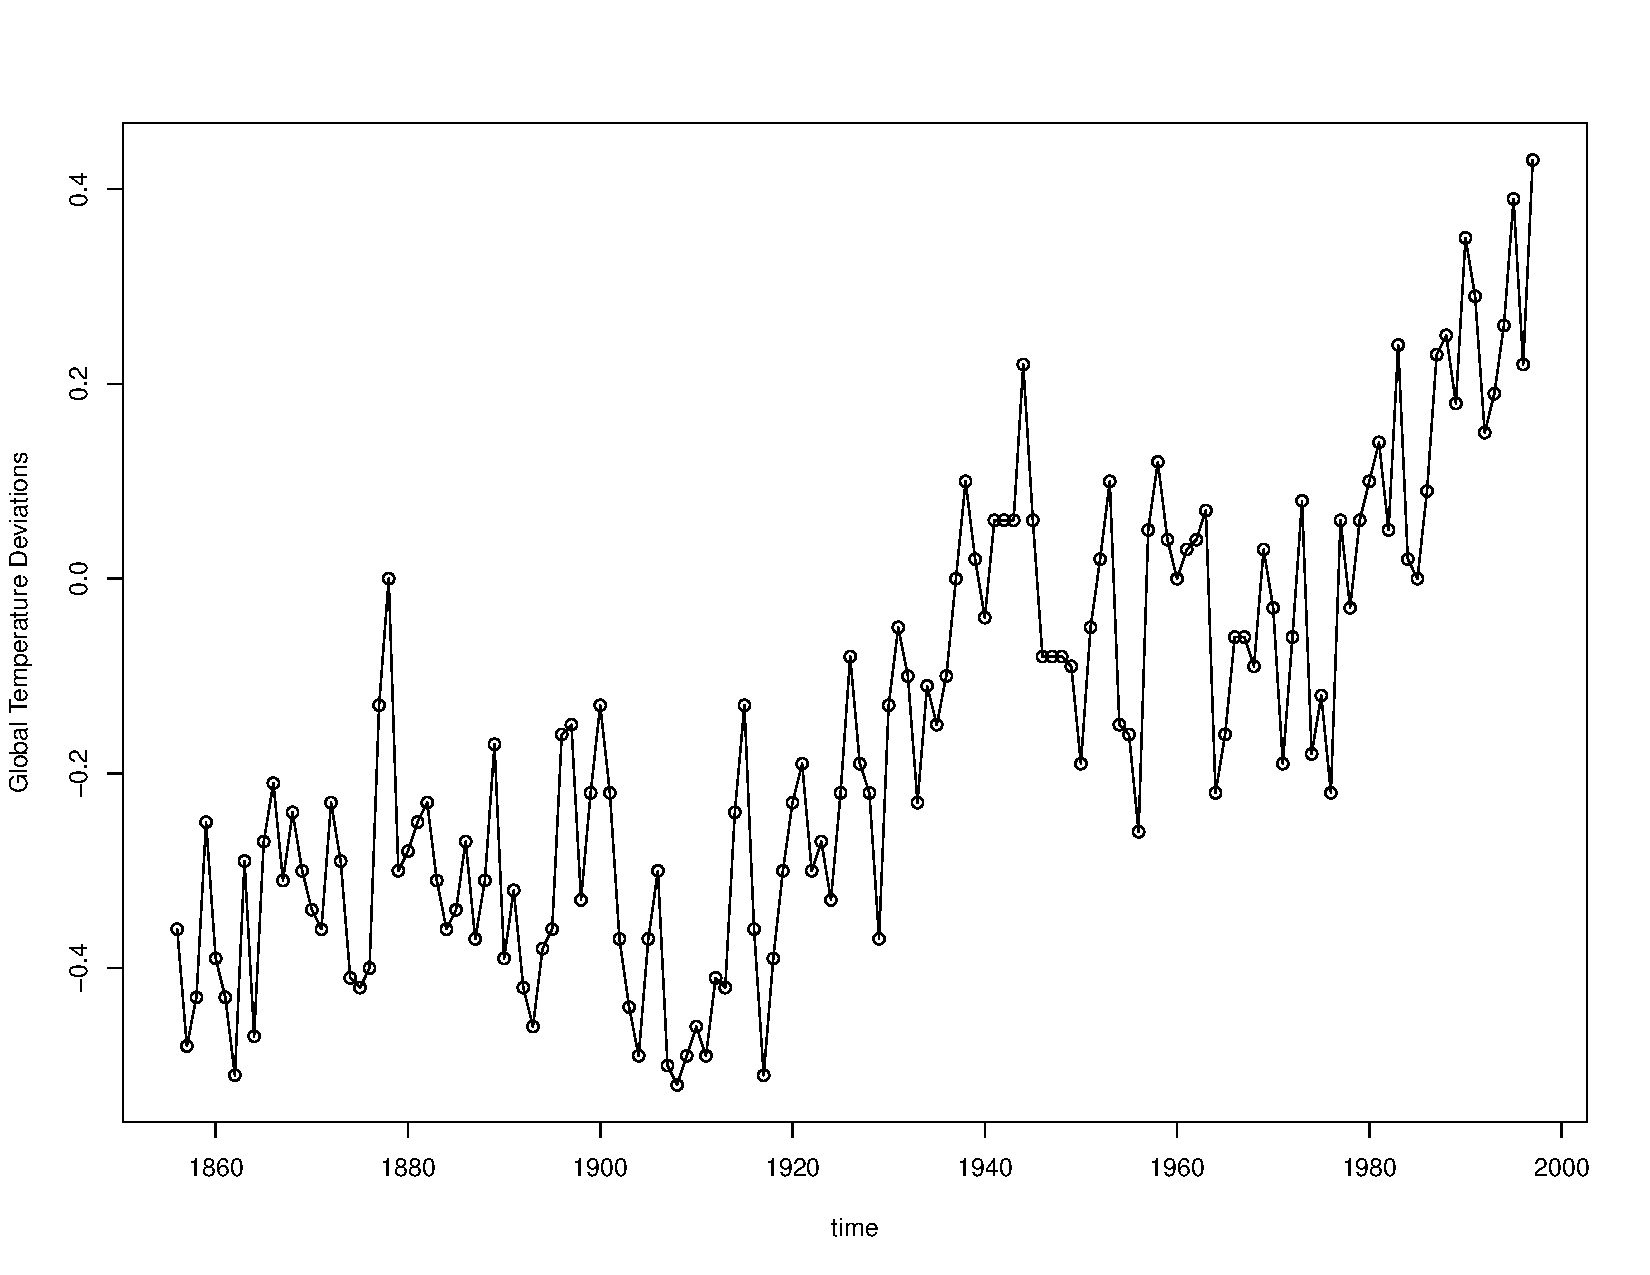
\includegraphics[width=\linewidth]{gtemp.pdf}}
	\caption{Cambio clim\'atico: mediciones de temperatura desde 1860}\label{figura1}
\end{figure}
%\end{frame}

%\centering
\lstset{caption=Código R para ejemplo del cambio climático,framexleftmargin=5mm, frame=shadowbox, rulesepcolor=\color{green}}
\pagebreak
\begin{lstlisting}[title={‘Código R  para ejemplo del cambio climático.’},basicstyle=\ttfamily]{}
# Set the working directory
setwd("/Users/Desktop/Econometrics/Clase 1.- TSE")
# Limpiar_variables
rm(list=ls())

install.packages("tidyverse")
install.packages("dplyr")
install.packages("tseries")

mydata<-read.csv ("gtemp.csv")
plot(mydata, type="o", ylab="Global Temperature Deviations")
\end{lstlisting}

%---------------------Slide 9 --------------------------
%\begin{frame}
\subsection{Ejemplo 2: Series temporales financieras}
%\frametitle{Ejemplo 2: Series temporales financieras}
En finanzas siempre es preferible trabajar con el retorno (returns) de los activos, en vez de usar directamente el precio de los activos. Existen dos maneras de convertir el precio en retornos:
\begin{equation*}
R_t = \frac{p_t - p_{t-1}}{p_{t-1}} *100%
\end{equation*}
\\
\begin{equation*}
R_t = ln\left(\frac{p_t}{p_{t-1}}\right)*100%
\end{equation*}
where, $R_t$ denota el retorno al tiempo $t$, $p_t$ denota el precio del activo al tiempo $t$, y $ln$ denota el logaritmo natural. En esta formulaci\'on ignoramos los dividendos, o asumimos que las series de precios ya han sido ajustadas por ellos.

%\end{frame}
%---------------------Slide 10 --------------------------
%\begin{frame}
%\frametitle{Ejemplo 2: Series temporales financieras}
Los log-returns tienen la deseable propiedad de poder ser interpretados como rendimientos continuamente compuestos. Adem\'as, ellos pueden ser simplemente sumados, de forma de obtener retornos con respecto a per\'\i{}odos m\'as largos:
\begin{center}
	$r_1 = ln \frac{p_1}{p_0} = ln p_1 - ln p_0$\\
	$r_2 = ln \frac{p2}{p_1} = ln p_2 - ln p_1$\\
	$r_3 = ln \frac{p3}{p_2} = ln p_3 - ln p_2$\\
	$r_4 = ln \frac{p4}{p_3} = ln p_4 - ln p_3$\\
	$r_5 = ln \frac{p5}{p_4} = ln p_5 - ln p_4$\\	
	\vspace{5mm}	     			      
	$r_1+r_2+r_3+r_4+r_5=ln p_5 - ln p_0    =  ln \frac{p_5}{p_0}$\\
\end{center}
%\end{frame}
%---------------------------------------------------------
%\begin{frame}
%\frametitle{Ejemplo 2: Series temporales financieras}
\subsubsection{Ejemplo 2: Series temporales financieras}
Como segundo ejemplo calcularemos los retornos de la Bolsa de Nueva York, \'\i{}ndice "S$\&$P 500", extrayendo data diaria desde el a\~no 2000, del sitio: https://finance.yahoo.com/\\

%\only<1|handout:1>{
	%\begin{exampleblock}{C\'odigo en R}
\lstset{caption=Código R precio de la Bolsa de Nueva York,framexleftmargin=5mm, frame=shadowbox, rulesepcolor=\color{green}}
\begin{lstlisting}[title={‘Código R precio de la Bolsa de Nueva York.’},basicstyle=\ttfamily]{}
mydata2<-read.csv("sp.csv")
precio<-mydata2$"Adj.Close"
plot.ts(precio, type="o", ylab="Precio Bolsa de Nueva York")
lnprecio <- log10(precio)
Dlnprecio <- diff(lnprecio,1)
plot.ts(Dlnprecio, type="o", ylab="Retorno Bolsa de Nueva York")
summary (lnprecio)
summary (Dlnprecio)
\end{lstlisting}

%\end{exampleblock}
%}
%\end{frame}
%---------------------------------------------------------
%---------------------Slide 12 --------------------------
%\begin{frame}
%\frametitle{Ejemplo 2: Series temporales financieras}
%\textbf{Indice Bolsa de Nueva York}
%\end{frame}
\begin{figure}[H]{}
\centering
\textbf{Ejemplo 2: Series temporales financieras}\par\medskip
\fcolorbox{green}{blue}{
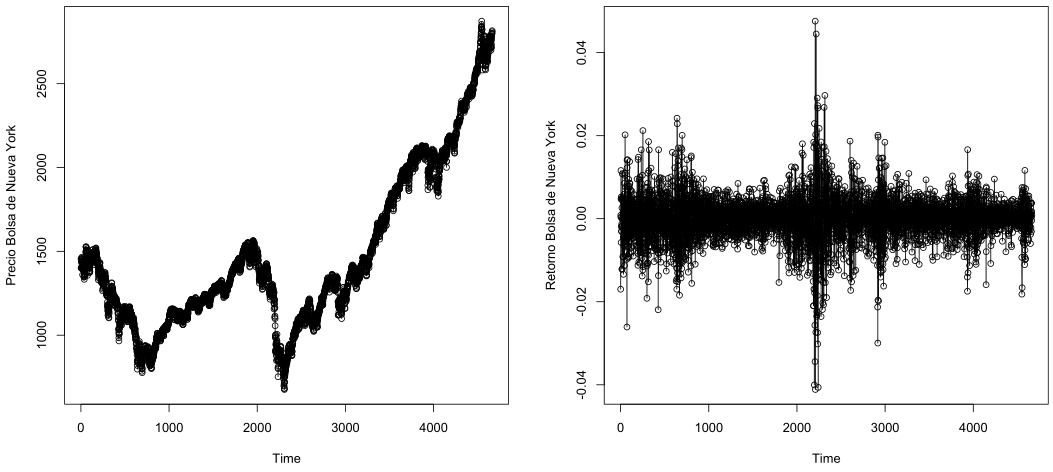
\includegraphics[width=\linewidth]{bolsaNYD12.png}}
\caption{Indice Bolsa de Nueva York. Izquierda: precios reales SP500. Derecha: retornos SP500.}\label{figura2}
\end{figure}

%---------------------------------------------------------
%---------------------Slide 13 --------------------------
%\begin{frame}
%\frametitle{Ejemplo 2: Series temporales financieras}
Los precios al parecer no son normales, aparentemente son log-normales.\\
\begin{figure}[H]
	\centering
	\textbf{Ejemplo 2: Histograma de los Precios}\par\medskip
	\fcolorbox{green}{blue}{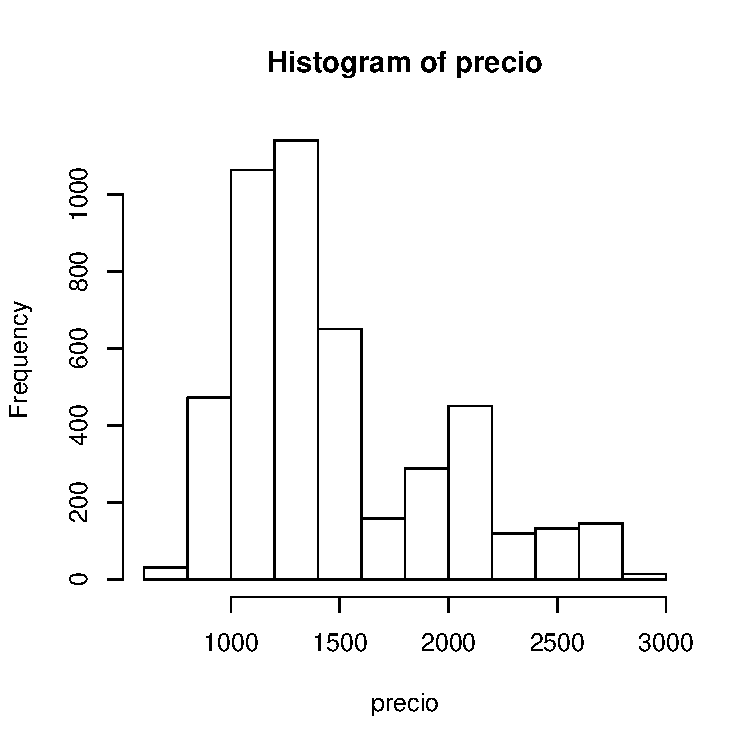
\includegraphics[width=\linewidth]{hist_precio_sp.pdf}}
	\caption{Histograma de los precios de la Bolsa de NY}\label{figura3}
\end{figure}
%\end{frame}

%---------------------------------------------------------
%---------------------Slide 14 --------------------------
%\begin{frame}
%\frametitle{Ejemplo 2: Series temporales financieras}
\pagebreak
Los retornos de los precios si parecen normales~\ref{figura4}, lo cual constituye una propiedad deseable para el an\'alisis estad\'\i{}stico.\\
\begin{figure}[H]
	\centering
	\textbf{Ejemplo 2: Histograma de los Precios}\par\medskip
	\fcolorbox{green}{blue}{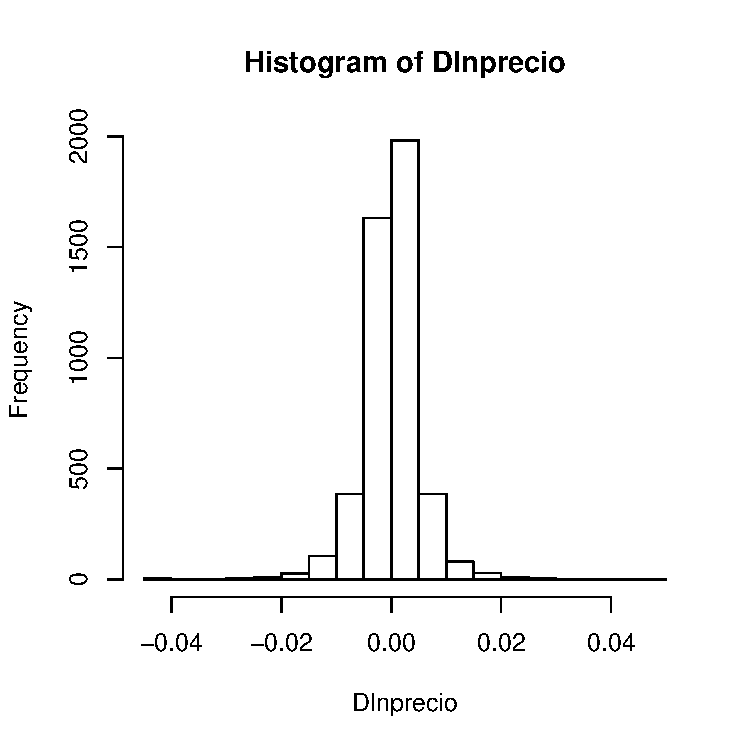
\includegraphics[width=\linewidth]{hist_dlnprecio_sp.pdf}}
	\caption{Histograma de los retornos de la Bolsa de NY}\label{figura4}
\end{figure}
%\end{frame}

%\end{section}
%---------------------------------------------------------
%---------------------Slide 15 --------------------------
%\begin{frame}
%\frametitle{Ejemplo 2: Series temporales financieras}
\begin{figure}[H]
	\centering
	\textbf{Ejemplo 2: Histograma de los Precios}\par\medskip
	\fcolorbox{green}{blue}{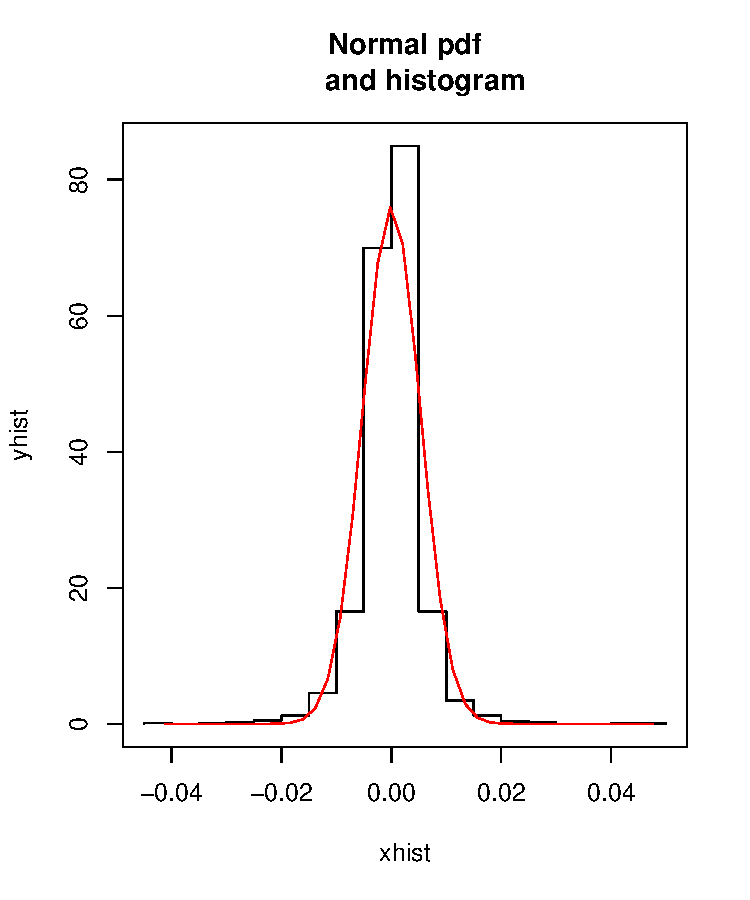
\includegraphics[width=\linewidth]{normal_hist_Dlnprice_sp.pdf}}
	\caption{Linea negra:Histograma de las diferencias de los log-precios de la Bolsa de NY. Linea roja: ajuste de la distribución normal segúun media y desviación estandar de la muestra. Shapiro-Wilk normality test / data:  Dlnprecio / W = 0.90927, p-value $<$ 2.2e-16.}\label{figura5}
\end{figure}
%Shapiro-Wilk normality test
%data:  Dlnprecio
%W = 0.90927, p-value $<$ 2.2e-16.
%\end{frame}

%---------------------------------------------------------
%---------------------Slide 16 --------------------------
%\begin{frame}
%\frametitle{Ejemplo 2: Series temporales financieras}
%
%\only<1|handout:1>{
	%\begin{exampleblock}{C\'odigo en R}
%		h $<-$ hist(Dlnprecio,breaks=15)\\
%		xhist $<-$ c(min(h\$breaks),h\$breaks)\\
%		yhist $<-$ c(0,h\$density,0)\\
%		xfit $<-$ seq(min(Dlnprecio),max(Dlnprecio),length=40)\\
%		yfit $<-$ dnorm(xfit,mean=mean(Dlnprecio),sd=sd(Dlnprecio))\\
%		plot(xhist,yhist,type="s",ylim=c(0,max(yhist,yfit)), main=``Normal pdf and histogram")\\
%		lines(xfit,yfit, col=``red")\\
%		shapiro.test(Dlnprecio)
	%\end{exampleblock}
%}
%\end{frame}
\pagebreak
\lstset{caption = Código R de histograma y ajuste de curva normal,framexleftmargin=5mm, frame=shadowbox, rulesepcolor=\color{green}}
\begin{lstlisting}[title={‘Código R de histograma y ajuste de curva normal’},basicstyle=\ttfamily]{}
h <- hist(Dlnprecio,breaks=15)
xhist <- c(min(h$breaks),h$breaks)
yhist <- c(0,h$density,0)
xfit <- seq(min(Dlnprecio),max(Dlnprecio),length=40)
yfit <- dnorm(xfit,mean=mean(Dlnprecio),sd=sd(Dlnprecio))
plot(xhist,yhist,type="s",ylim=c(0,max(yhist,yfit)), 
	main="Normal pdf and histogram")
lines(xfit,yfit, col="red")
shapiro.test(Dlnprecio)
\end{lstlisting}

%---------------------------------------------------------
%---------------------Slide 17 --------------------------
%\begin{section}{Modelamiento estad\'istico de las series de tiempo}
\section{Modelamiento estad\'istico de las series de tiempo}
%	\begin{frame}
%	\frametitle{Modelos estad\'isticos de series de tiempo}
	Para poder modelar los datos, que aparentemente fluct\'uan de forma aleatoria a lo largo del tiempo, suponemos que una serie temporal se define como una colecci\'on de variables aleatorias. 
	\\
	Por ejemplo, podemos modelar  una serie temporal como una secuencia de variables aleatorias, $x_1, x_2, x_3,...$, donde la variable aleatoria $x_1$ denota el valor tomado por la serie en el primer punto de tiempo, la variable $x_2$  denota el valor para el segundo per\'\i{}odo de tiempo, y as\'\i{} sucesivamente. 
	\\
	En general, una colecci\'on de variables aleatorias,  $\{x_t\}$, indexada por t se conoce como proceso estoc\'astico. En este texto, $t$ ser\'a t\'\i{}picamente discreto y variar\'a sobre los enteros $t = 0, \pm1, \pm2,,.... $, o alg\'un subconjunto de los enteros. Los valores observados en un proceso estoc\'astico se conocen como la realizaci\'on del proceso estoc\'astico.	
%\end{frame}
%---------------------------------------------------------
%---------------------Slide 18 --------------------------
%\begin{frame}
%\frametitle{Ruido blanco - White Noise}
\subsection{Ruido blanco - White Noise}
Una serie de tiempo muy utilizada es aquella representada por una colecci\'on de variables aleatorias no correlacionadas, $\epsilon_t$, con media $0$ y varianza finita $\sigma^2_\epsilon$. Las series temporales generadas a partir de variables no correlacionadas se utilizan por ejemplo para modelar el ruido en aplicaciones de ingenier\'\i{}a, donde se denomina ruido blanco. A veces denotaremos este proceso como $\epsilon_t$$\sim$$\epsilon_n (0, \sigma^2_\epsilon)$. La designaci\'on de "blanco" se origina de la analog\'\i{}a con la luz blanca e indica que todas las posibles oscilaciones peri\'odicas est\'an presentes con la misma fuerza.

%\end{frame}
%---------------------------------------------------------
%---------------------Slide 19 --------------------------
%\begin{frame}
%\frametitle{Ruido blanco - White Noise}

\begin{itemize}
	\item En ocasiones, tambi\'en requeriremos que el ruido sea independiente y tenga una distribuci\'on id\'entica (iid) de variables aleatorias con media 0 y varianza $\sigma^2_\epsilon$. Distinguiremos este caso diciendo ruido blanco independiente, o escribiendo $\epsilon_t$ $\sim$ $iid (0, \sigma^2_\epsilon)$. 
	\item Otra serie de ruido blanco particularmente \'util es el ruido blanco gaussiano, en el que las $w_t$ son variables aleatorias normales independientes, con media $0$ y varianza $\sigma^2_\epsilon$; o m\'as sucintamente, $\epsilon_t \sim iid \hspace{0.1cm}N(0, \sigma^2_\epsilon)$. 
	\item La figura siguiente muestra una colecci\'on de 500 de estas variables aleatorias, con $\sigma^2_\epsilon=1$, trazadas en el orden en que se dibujaron.
\end{itemize}

%\end{frame}
%---------------------------------------------------------
%---------------------Slide 20 --------------------------
%\begin{frame}
%\frametitle{Ruido blanco - White Noise}
%
%\only<1|handout:1>{
%	\begin{exampleblock}{C\'odigo en R}
%		set.seed(154) \\
%		w = rnorm(200,0,1) \\
%		plot.ts(w, ylim=c(-3,3), main="White Noise") \\
%	\end{exampleblock}
%}
%\begin{figure}[t!]
%	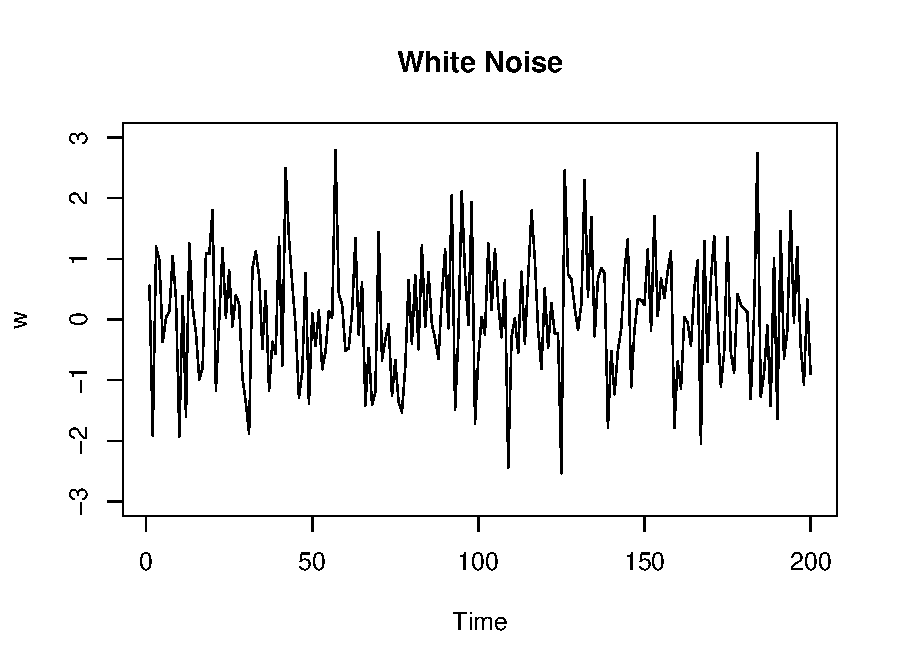
\includegraphics[scale=0.3]{white_noise.pdf}
%\end{figure}
%
%\end{frame}
\lstset{caption = Código R para generar Ruido blanco,framexleftmargin=5mm, frame=shadowbox, rulesepcolor=\color{green}}
\begin{lstlisting}[title={‘Código R para generar Ruido blanco’},basicstyle=\ttfamily]{}
set.seed(154)
w = rnorm(200,0,1)
plot.ts(w, ylim=c(-3,3), main="White Noise")
\end{lstlisting}\label{codigoRuidoBlanco}

\begin{figure}[H]
	\centering
	\textbf{Ruido blanco - White Noise}\par\medskip
	\fcolorbox{green}{blue}{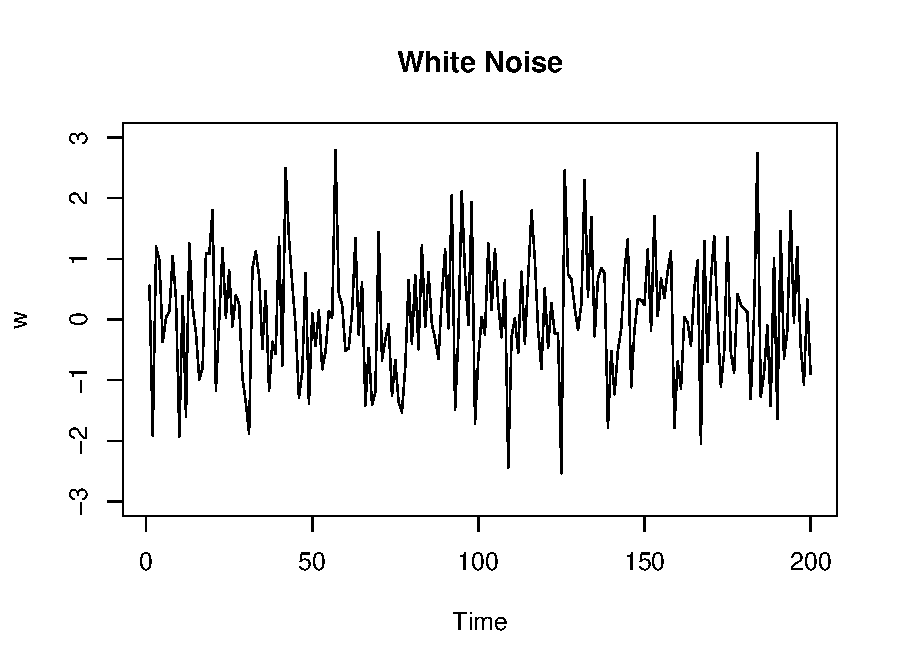
\includegraphics[width=\linewidth]{white_noise.pdf}}
	\caption{Ruido blanco - White Noise}\label{figura6}
\end{figure}

%---------------------------------------------------------
%---------------------Slide 21 --------------------------
%\begin{frame}
%\frametitle{Caminata Aleatoria - Random Walk}
\subsection{Caminata Aleatoria - Random Walk}

Un ejemplo simple para modelar una serie temporal estoc\'astica con tendencia (no estacionaria) es una caminata aleatoria con deriva (Random Walk with drift):

\begin{equation*}
x_t = \delta + x_{t-1} + \epsilon_t 
\end{equation*}

para $t = 1, 2,. . .$, con una condici\'on inicial $x_0 = 0$, y donde $\epsilon_t$ es ruido blanco. La constante $\delta$ se denomina deriva (drift), y cuando $\delta=0$, se llama simplemente una caminata aleatoria. El t\'ermino caminata aleatoria proviene del hecho de que, cuando $\delta=0$, el valor de la serie de tiempo en el tiempo $t$, es el valor de la serie en el tiempo $t - 1$ m\'as un movimiento completamente aleatorio determinado por $\epsilon_t$. 
%\end{frame}

%---------------------------------------------------------
%---------------------Slide 22 --------------------------
%\begin{frame}
%\frametitle{Caminata Aleatoria - Random Walk}

Tenga en cuenta que podemos reescribir la ecuaci\'on anterior como una suma acumulativa de las variables de ruido blanco. Es decir,

\begin{equation*}
x_t = \delta t + \sum_{j=1}^{t} \epsilon_t 
\end{equation*}

%\end{frame}
%---------------------------------------------------------
%---------------------Slide 23 --------------------------
%\begin{frame}
%\frametitle{Caminata Aleatoria - Random Walk}

%\only<1|handout:1>{
%	\begin{exampleblock}{C\'odigo en R}
%		set.seed(154) \\
%		w = rnorm(200,0,1) \\
%		x = cumsum(w) \\
%		wd = w + 0.2 \\
%		xd = cumsum(wd) \\
%		plot.ts(xd, ylim=c(-5,55), main=``random walk") \\
%		lines(x) \\
%		lines(0.2*(1:200), lty=``dashed") \\
%	\end{exampleblock}
%}
%\end{frame}
\lstset{caption = Código R para generar Caminata Aleatoria,framexleftmargin=5mm, frame=shadowbox, rulesepcolor=\color{green}}
\begin{lstlisting}[title={‘Código R para generar Caminata Aleatoria’},basicstyle=\ttfamily]{}
set.seed(154)
w = rnorm(200,0,1)
x = cumsum(w)
wd = w + 0.2
xd = cumsum(wd)
plot.ts(xd, ylim=c(-5,55), main="random walk")
lines(x)
lines(0.2*(1:200), lty="dashed")
\end{lstlisting}\label{codigoCaminataAleatoria}

%---------------------------------------------------------
%---------------------Slide 24 --------------------------
%\begin{frame}
%\frametitle{Caminata Aleatoria - Random Walk}

\begin{figure}[H]
	\centering
	\textbf{Caminata aleatoria}\par\medskip
	\fcolorbox{green}{blue}{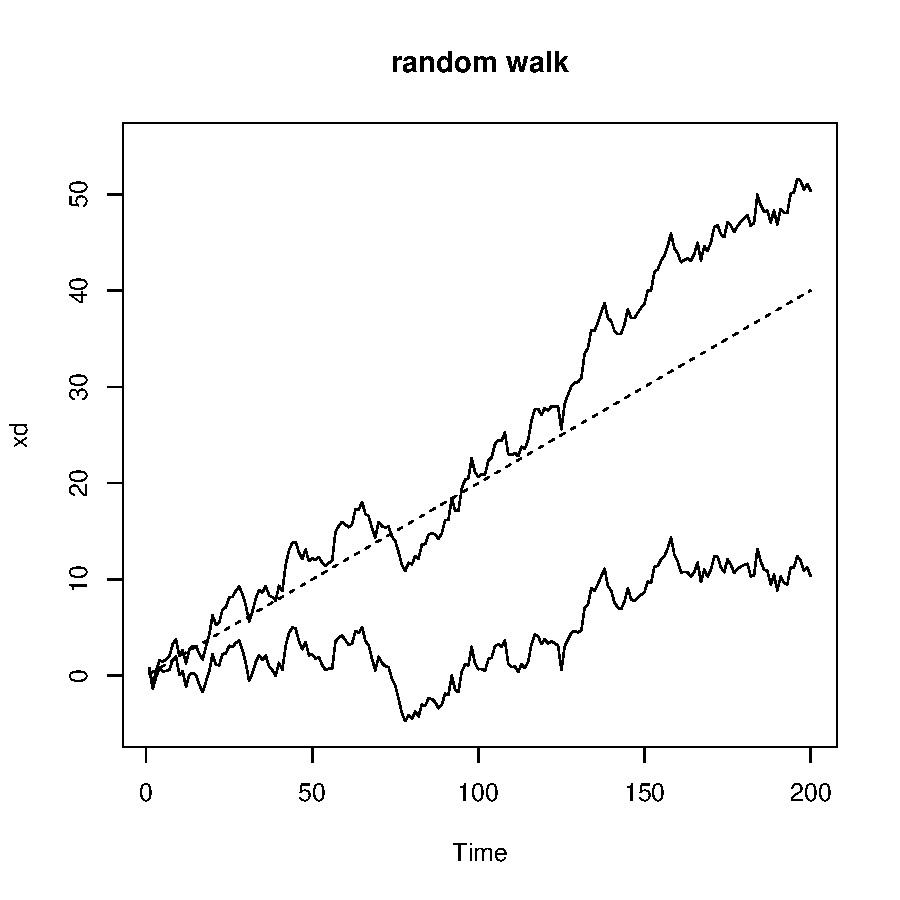
\includegraphics[width=\linewidth]{random_walk.pdf}}
%	\textbf{Random Walk}\par\medskip
%	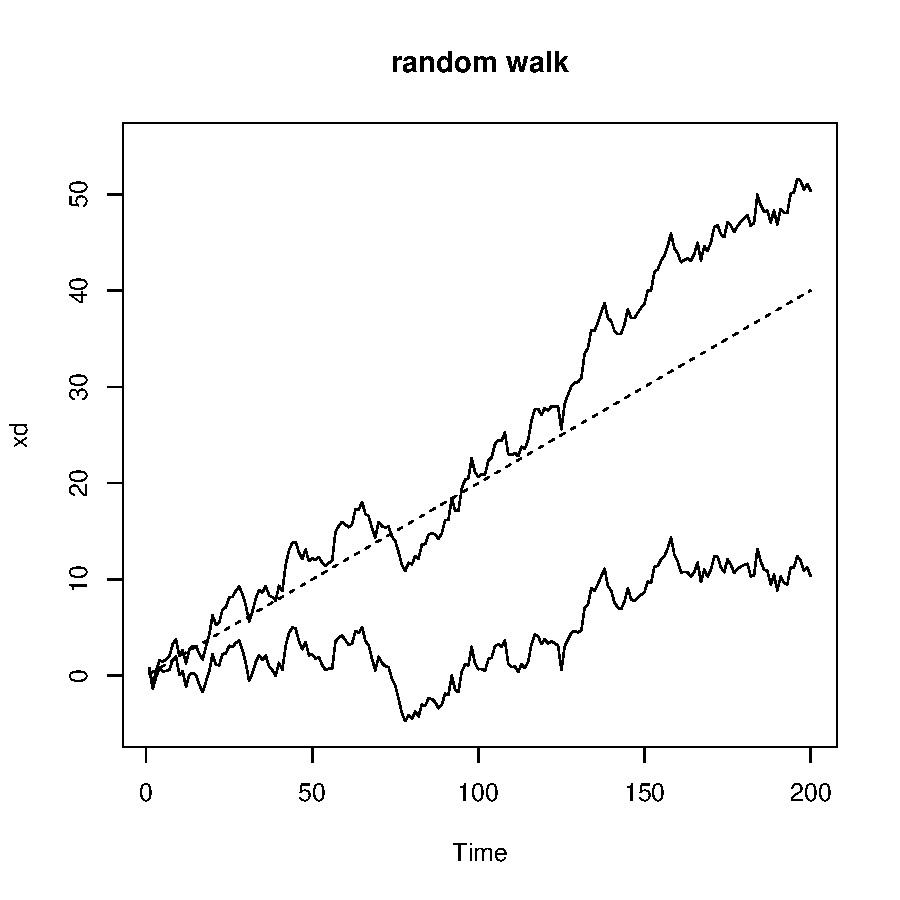
\includegraphics[scale=0.6]{random_walk.pdf}
	\caption{Caminata Aleatoria - Random walk, $\sigma_\epsilon$ = 1, with drift $\delta =0 .2$ (upper jagged line), without drift, $\delta = 0$ (lower jagged line), and a straight line with slope 0.2 (dashed line).}\label{figura7}
\end{figure}

%---------------------------------------------------------
%---------------------Slide 25 --------------------------
%\begin{frame}
%\frametitle{Promedios m\'oviles - Moving Averages}
\pagebreak\subsection{Promedios m\'oviles - Moving Averages}
Podr\'\i{}amos reemplazar la serie de ruido blanco $\epsilon_t$ por un promedio m\'ovil que suavice la serie. Por ejemplo, considere reemplazar $\epsilon_t$ por un promedio de su valor actual y sus vecinos inmediatos en el pasado y futuro. Es decir:

\begin{equation*}
v_t = 1/3 (\epsilon_{t-1} + \epsilon_t + \epsilon_{t+1})
\end{equation*}

Como veremos en el siguiente ejemplo, los promedios m\'oviles producen una versi\'on m\'as suave que la serie original, lo que refleja el hecho de que las oscilaciones m\'as lentas llegan a ser m\'as evidentes, y se eliminan algunas de las oscilaciones m\'as r\'apidas. 

%\end{frame}
%---------------------------------------------------------
%---------------------Slide 26 --------------------------
%\begin{frame}
%\frametitle{Promedios m\'oviles - Moving Averages}

%\only<1|handout:1>{
%	\begin{exampleblock}{C\'odigo en R}
%		w = rnorm(500,0,1) ; v = filter(w, sides=2, rep(1/3,3)) 
%		par(mfrow=c(2,1))\\
%		plot.ts(w, main=``white noise"); plot.ts(v, main=``moving average")\\
%	\end{exampleblock}
%}
\lstset{caption = Código R para generar Promedios móviles,framexleftmargin=5mm, frame=shadowbox, rulesepcolor=\color{green}}
\begin{lstlisting}[title={‘Código R para generar Moving Averages’},basicstyle=\ttfamily]{}
w = rnorm(500,0,1) ; v = filter(w, sides=2, rep(1/3,3))
par(mfrow=c(2,1))
plot.ts(w, main="white noise")
plot.ts(v, main="moving average")
\end{lstlisting}\label{movingAverage}
\begin{figure}[H]
	\centering
	\textbf{Medias móviles}\par\medskip
	\fcolorbox{green}{blue}{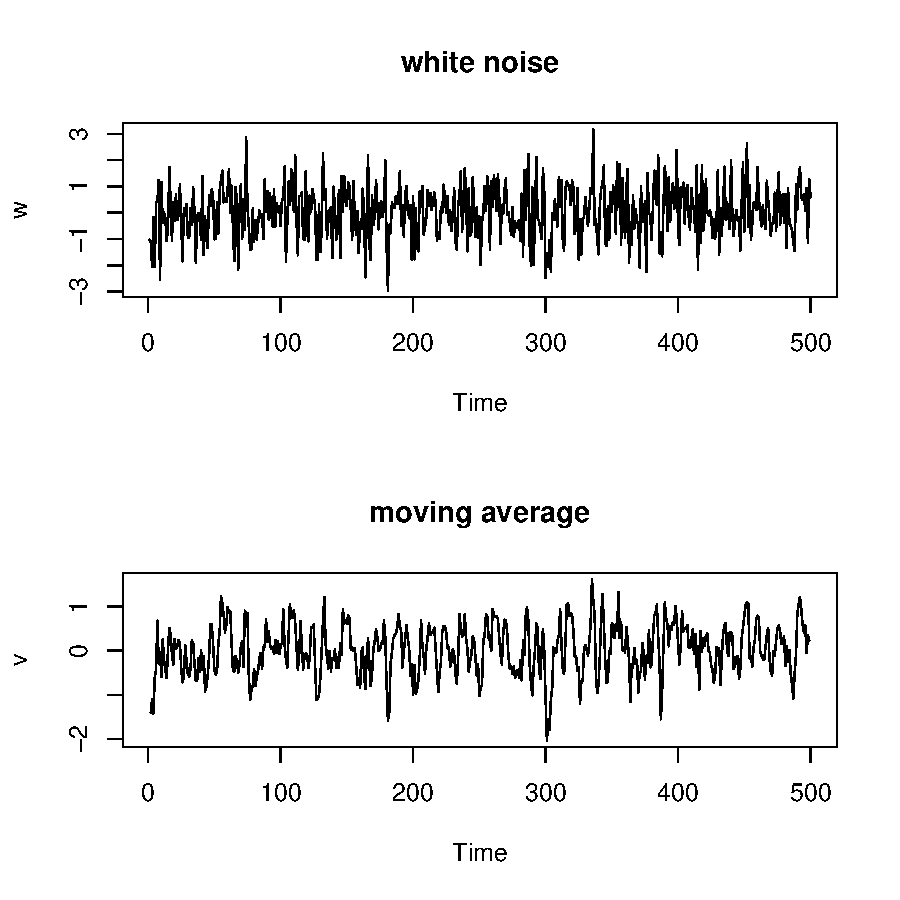
\includegraphics[width=\linewidth]{moving_average.pdf}}
%	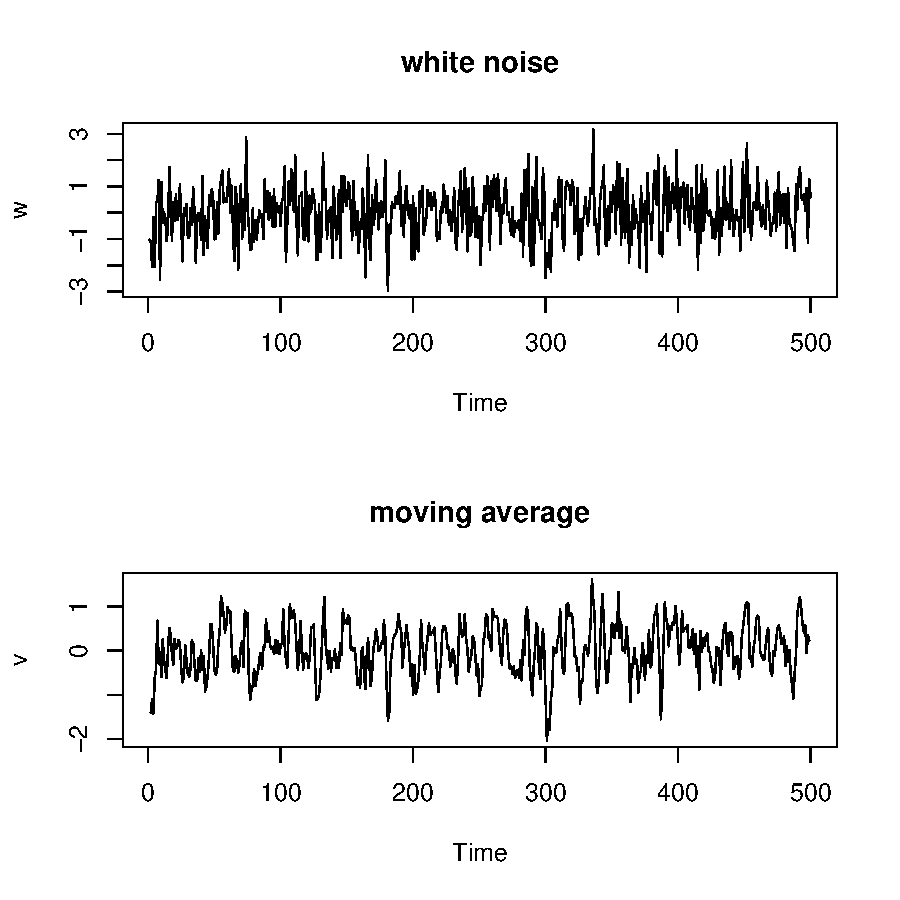
\includegraphics[scale=0.7]{moving_average.pdf}
	\caption{Promedios Móviles - Moving Averages}\label{figura8}
\end{figure}

%\end{frame}



%\end{frame}
%---------------------------------------------------------
%---------------------Slide 27 --------------------------
%\begin{frame}
%\frametitle{Autorregresiones - Autoregressions}
\subsection{Autorregresiones - Autoregressions}
Supongamos nuevamente que consideramos la serie de ruido blanco $w_t$ como entrada, y calculamos la salida usando una ecuaci\'on de segundo orden, es decir:

\begin{equation*}
x_t = x_{t-1} - 0.9 x_{t-2} + \epsilon_t
\end{equation*}

Esta ecuaci\'on representa una regresi\'on o predicci\'on del valor actual $x_t$ de una serie temporal en funci\'on de los dos valores anteriores de la serie, es por esto que utilizamos el nombre de autoregresi\'on.

%\end{frame}

%---------------------------------------------------------
%---------------------Slide 28 --------------------------
%\begin{frame}
%\frametitle{Autorregresiones - Autoregressions}

%\only<1|handout:1>{
%\begin{exampleblock}{C\'odigo en R}
%	w = rnorm(550,0,1) ; x = filter(w, filter=c(1,-.9), method= ``recursive")[-(1:50)]\\
%	plot.ts(x, main= ``autoregression")
%\end{exampleblock}
%}
\lstset{caption = Código R para generar Auto regresiones,framexleftmargin=5mm, frame=shadowbox, rulesepcolor=\color{green}}
\begin{lstlisting}[title={‘Código R para generar Autoregresions’},basicstyle=\ttfamily]{}
w = rnorm(550,0,1) ; 
x = filter(w, filter=c(1,-.9), method="recursive")[-(1:50)]
plot.ts(x, main= "autoregression")
\end{lstlisting}\label{autoregression}
\begin{figure}[H]
	\centering
	\textbf{Autorregresiones}\par\medskip
	\fcolorbox{green}{blue}{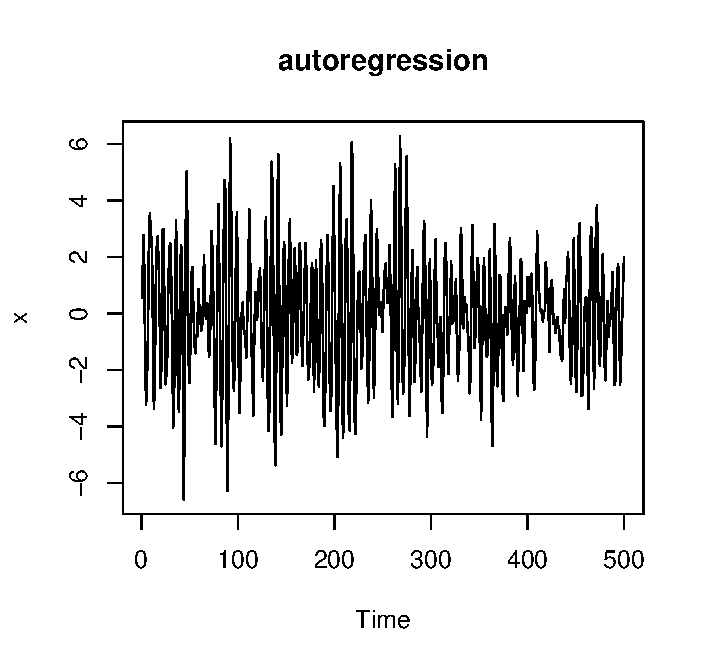
\includegraphics[width=\linewidth]{autoregression.pdf}}
%	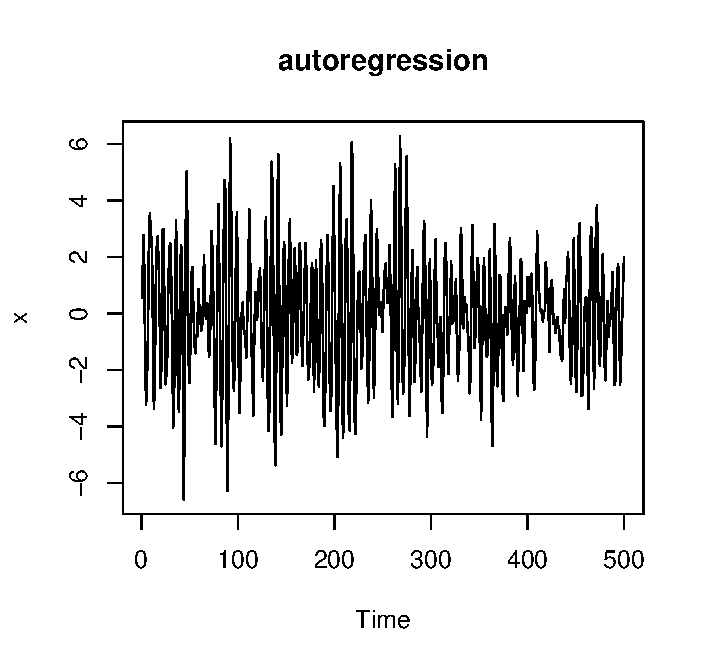
\includegraphics[scale=0.7]{autoregression.pdf}
	\caption{Autorregresiones - Autoregressions}\label{figura9}
\end{figure}

%---------------------------------------------------------
%---------------------Slide 29 --------------------------
\pagebreak\section{Descomposici\'on de las series de tiempo}
%	\begin{frame}
%	\frametitle{Descomposici\'on de las series de tiempo}	
Las series de tiempo usualmente se descomponen en:
	\begin{itemize}
		\item Una tendencia (trend) $T_t$. 
		\item Un componente estacional (seasonal) $S_t $.
		\item Un elemento irregular (irregular) $I_t$.
	\end{itemize}
	\vspace{5mm}
Por ejemplo:
	\begin{center}
		\vspace{3mm}
		$T_t=2+0.1 t$; \\
		\vspace{3mm}
		$S_t = 6.5 cos (\pi/60)$; \\
		\vspace{3mm}
		y $I_t\sim$ $N(\mu=0, \sigma^2=0.5)$. 
	\end{center}
%---------------------------------------------------------
%---------------------Slide 30 --------------------------
%\begin{frame}
%\frametitle{Descomposici\'on de las series de tiempo}
%
%\only<1|handout:1>{
%	\begin{exampleblock}{C\'odigo en R}
%		rm(list=ls())\\
%		$t = 2 + 0.1*1:500$\\
%		$s = 6.5*cos(pi*1:500/90)$\\
%		set.seed(154) \\
%		$i = rnorm(500,0,5)$\\
%		$plot.ts(s+t+i)$\\
%	\end{exampleblock}
%}
%\end{frame}
\lstset{caption = Código R para descomponer serie de tiempo,framexleftmargin=5mm, frame=shadowbox, rulesepcolor=\color{green}}
\begin{lstlisting}[title={‘Código R para descomponer serie de tiempo’},basicstyle=\ttfamily]{}
t = 2 + 0.1 * 1:500
s = 6.5 * cos(pi * 1:500/90)
set.seed(154)
i = rnorm(500, 0, 5)
plot.ts(s + t + i)
\end{lstlisting}\label{descomposicionTS}

%---------------------------------------------------------
%---------------------Slide 31 --------------------------
%\begin{frame}
%\frametitle{Descomposici\'on de las series de tiempo}
\begin{figure}[H]
	\centering
	\textbf{Componentes de uuna Serie de Tiempo}\par\medskip
	\fcolorbox{green}{blue}{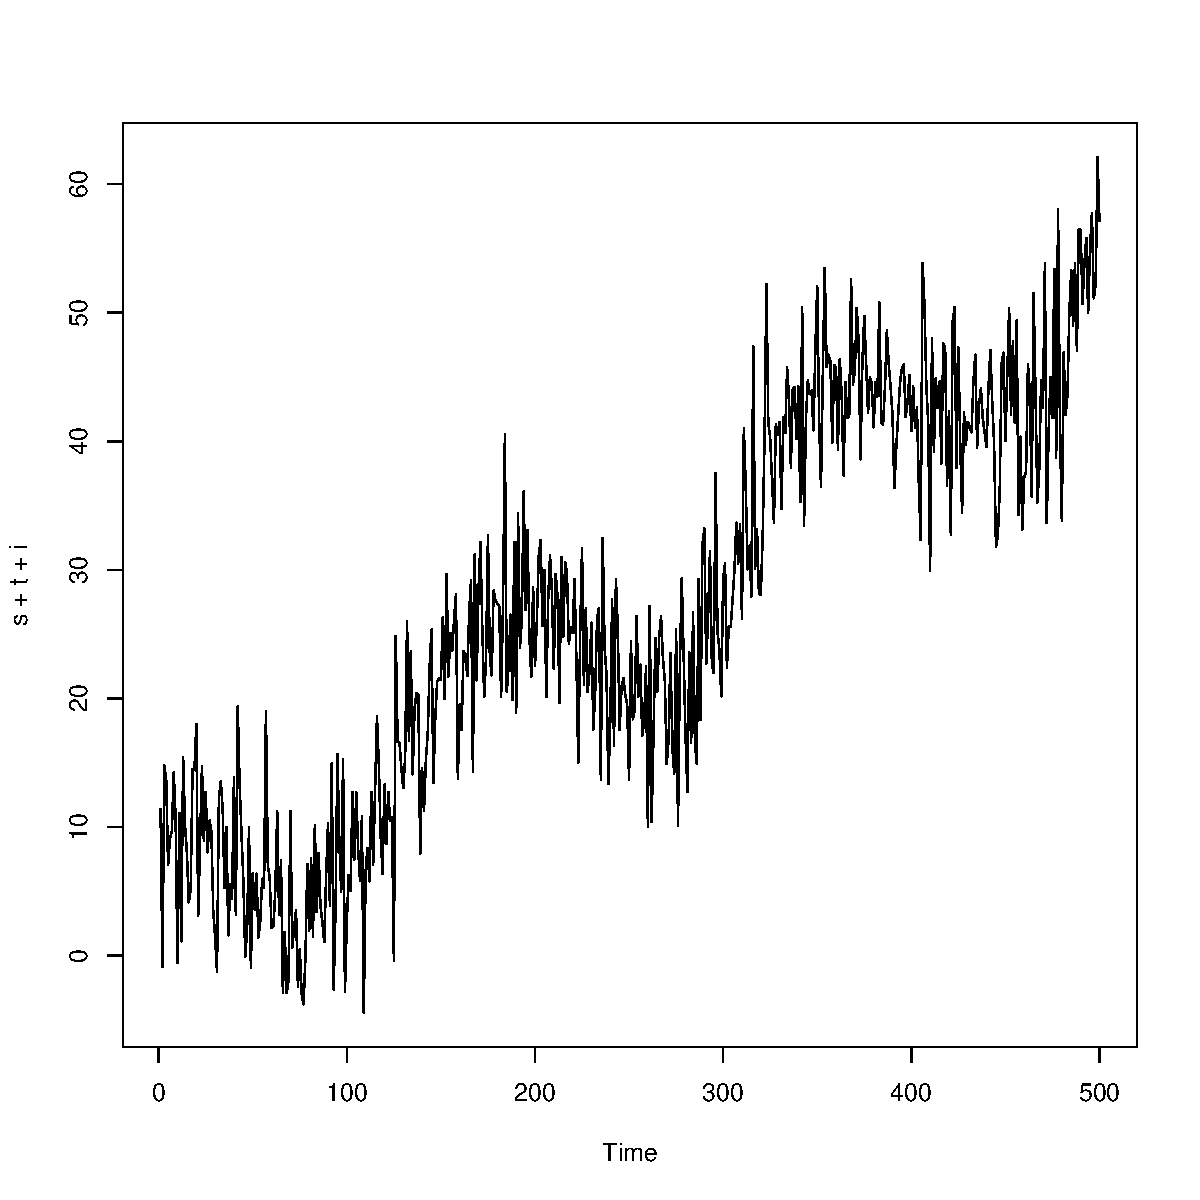
\includegraphics[width=\linewidth]{time_series.pdf}}
%	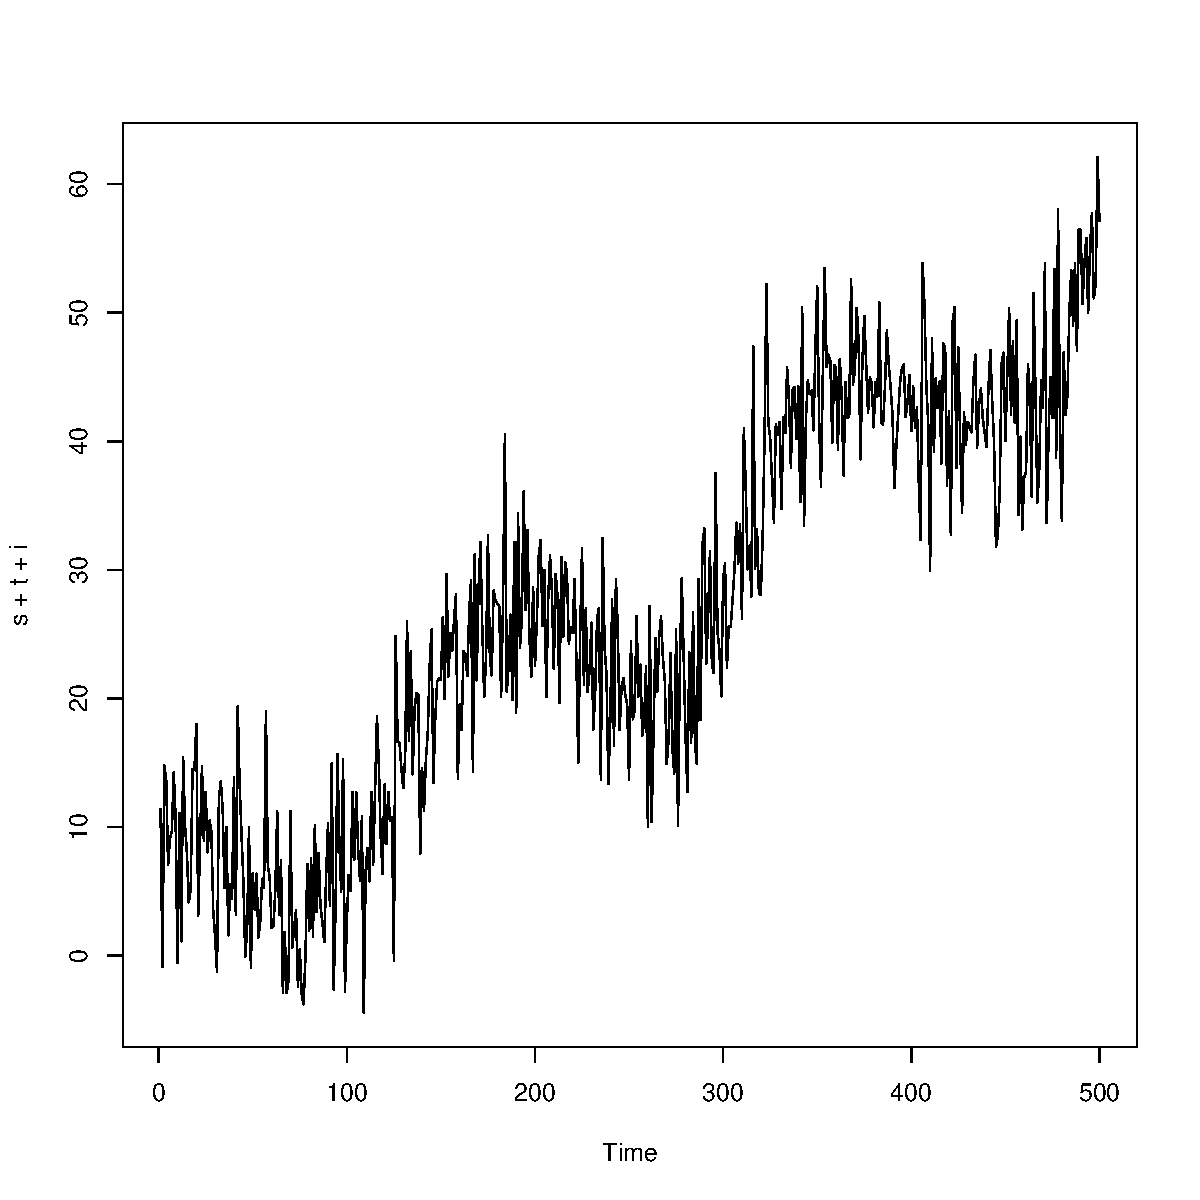
\includegraphics[scale=0.5]{time_series.pdf}
	\caption{Serie de tiempo con sus componentes T, S e I.}\label{figura10}
\end{figure}
%\end{frame}
%---------------------------------------------------------
%---------------------Slide 32 --------------------------
%\begin{frame}
%\frametitle{Descomposici\'on de las series de tiempo}

En general, las series de tiempo pueden contener uno o combinaci\'on de todos los elementos antes se\~nalados, ya sea de manera aditiva o multiplicativa:

\begin{equation*}
x_t = T_t + S_t + I_t
\end{equation*}

\begin{equation*}
x_t = T_t * S_t * I_t
\end{equation*}

\begin{itemize}
\item La primera especificaci\'on se caracteriza por tener cada componente de forma independiente, lo que posibilita descomponer la serie en una suma de los tres factores.
\item  La segunda, por otra parte, surge cuando la tendencia $(T_t)$, estacionalidad $(S_t)$, y irregularidad $(I_t)$ son dependientes entre si.
\end{itemize}

%\end{frame}

%---------------------------------------------------------
%---------------------Slide 33 --------------------------
%\begin{frame}
%\frametitle{Descomposici\'on de las series de tiempo}

En general, la tendencia cambia la media de la serie, mientras que el componente estacional posee un patr\'on que se repite, por ejemplo de manera mensual o trimestral. El componente irregular a pesar de no tener un patr\'on bien definido, puede ser pronosticada, de hecho, los pron\'osticos usan correlaciones con el componente irregular para realizar sus pron\'osticos. En per\'\i{}odos m\'as largos sin embargo, el componente irregular exhibe una tendencia de reversi\'on a cero.\\
El pron\'ostico de series de tiempo pretende entonces predecir cada uno de \'estos componentes de manera individual. Como vimos, el pron\'ostico global de la series de tiempo agrupa de forma aditiva o multiplicativa cada uno de dichos componentes.

%---------------------------------------------------------
%---------------------Slide 34 --------------------------
%\begin{frame}
%\frametitle{Descomposici\'on Tendencia\\
\subsection{Descomposici\'on Tendencia - Filtro Hodrick -Prescott}

\begin{itemize}
	\item En econom\'\i{}a, el filtro Hodrick-Prescott (HP) permite separar para $x_t$  los componentes tendencial y c\'\i{}clico.
	\item Este m\'etodo consiste en obtener una serie suavizada $S_t$ a partir de la original $x_t$, mediante una soluci\'on al problema de optimizaci\'on sugerido en la siguiente ecuaci\'on. Una vez resuelto, permite estimar tanto el ciclo como la tendencia de la serie.
\end{itemize}

\begin{equation*}
min \sum_{t=1}^{n} \left(x_t -S_t\right)^2 + \lambda \sum_{t=2}^{n-1} \left[ \left(S_{t+1}-S_t\right)-\left(S_t-S_{t-1}\right)\right]^2
\end{equation*}

\begin{itemize}
	\item Los valores sugeridos para $\lambda$ dependen de la periodicidad de $x_t$, y son: 14400 (mensual), 1600 (trimestral) y 100 (anual). Por otra parte, una vez obtenido el componente c\'\i{}clico $ \left(x_t -S_t\right)$, a partir del filtro HP, puede ser interpretada como la brecha existente entre su valor real $x_t$ y potencial $S_t$.
\end{itemize}

%---------------------------------------------------------
%---------------------Slide 35 --------------------------
%\begin{frame}
%\frametitle{Descomposici\'on componente estacional\\ 	Transformaciones de Diferencias}
\subsection{Descomposici\'on componente estacional - Transformaciones de Diferencias}

La transformaciones de diferencias se usan para capturar el componente estacional de la serie:

Una primera diferencia es definida como:

\begin{equation*}
\triangle x_t = (x_t - x_{t-1})
\end{equation*}

An\'alogamente, la segunda diferencia es definida como:

\begin{equation*}
\triangle^2x_t = (x_t - x_{t-1})-(x_{t-1} - x_{t-2})
\end{equation*}
Anteriormente vimos que la primera diferencia del logaritmo, se pod\'\i{}a interpretar como el cambio porcentual de la variable, logrando la simetr\'\i{}a del precio de las acciones.

%---------------------------------------------------------

%---------------------Slide 36 --------------------------
%\begin{frame}
%\frametitle{Descomposici\'on componente estacional\\
%	Variables Dummy}
\subsection{Descomposici\'on componente estacional - Variables Dummy}
Una variable dummy, D, es una variable binaria que toma la siguiente forma:

\begin{itemize}
	\item D=1  si la observaci\'on tiene caracter\'\i{}sticas espec\'\i{}ficas.
	\item D=0 si no las tiene.
\end{itemize}

Por ejemplo:

\begin{equation*}
x_t  = \beta_0 + \beta_1 z_t + \beta_2 D + \beta_3 D z_t
\end{equation*}

\begin{equation*}
D=1 => x_t  = (\beta_0 + \beta_2) + (\beta_1 + \beta_3) z_t
\end{equation*}

\begin{equation*}
D=0 => x_t  = \beta_0 + \beta_1 z_t
\end{equation*}

Las variables dummy pueden ser usadas para cambiar la pendiente y/o intercepto en un modelo lineal, lo cual permite capturar la estacionalidad en la serie, por ejemplo con variables dummys por trimestre o temporada.
%---------------------------------------------------------
%---------------------Slide 37 --------------------------
%\begin{section}{Medidas de dependencia}
%	\begin{frame}
%	\frametitle{Medidas de dependencia}
\pagebreak\section{Medidas de dependencia}
	Como vimos anteriormente, una serie de tiempo puede ser vista como una colecci\'on de n variables aleatorias en puntos de tiempo enteros arbitrarios $t_1, t_2,\cdots, t_n$, para cualquier entero positivo se cuenta con una funci\'on de distribuci\'on conjunta, evaluada como la probabilidad que los valores de las series sean conjuntamente menores que n constantes, $c_1, c_2,\cdots, c_n$, i.e.:
	\begin{equation*}
	F(c_1, c_2,\cdots, c_n) =  P(x_{t_1},\le c_1, x_{t_2} 	\le c_2,\cdots x_{t_n} \le c_n)
	\end{equation*}

%\end{frame}
%---------------------------------------------------------
%---------------------Slide 38 --------------------------
%\begin{frame}
%\frametitle{Medidas de dependencia}

Desafortunadamente, la funci\'on de distribuci\'on multinomial no puede usualmente ser escrita f\'acilmente a menos que las variables sean conjuntamente normales, en cual caso la densidad conjunta presenta la forma:
\begin{equation*}
f(\textbf{x}) = (2\pi)^{-2/n}\mid\Gamma\mid^{-1/2} exp \{ -1/2  (\textbf{x} - \mu)' \Gamma^{-1}\ (\textbf{x} - \mu)\}
\end{equation*}

donde $\mid\cdot\mid$ indica determinante y $\Gamma$ la matriz de covarianza.\\
Aunque la funci\'on de distribuci\'on conjunta permite describir la data completamente, su manipulaci\'on es muy compleja, y su despliegue gr\'afico imposible.
%\end{frame}
%---------------------------------------------------------
%---------------------Slide 39 --------------------------
%\begin{frame}
%\frametitle{Medidas de dependencia}

Las funciones de distribuci\'on marginales:
\begin{equation*}
F_t(x) = P\{x_t \le x\}
\end{equation*}

o la correspondiente funci\'on de densidad marginal:\\
\begin{equation*}
f_t(x) = \frac{\partial F_t(x)}{\partial x} 
\end{equation*}
\\
Cuando \'estas existen, proveen informaci\'on valiosa para examinar el comportamiento marginal de la serie.
\\
Si $x_t$ es Gausiana con media $\mu_t$ y varianza $\sigma_t^2$, $x_t$ $\sim$ $N(\mu_t,\sigma_t^2)$, la densidad marginal esta dada por:

\begin{equation*}
f_t(x) = \frac{1}{\sigma_t \sqrt{2 \pi}} exp  ( -  \frac{1}{2 \sigma_t^2}  (\textbf{x} - \mu_t)^2 )
\end{equation*}
%\end{frame}

%---------------------------------------------------------
%---------------------Slide 40 --------------------------
%\begin{frame}
%\frametitle{Medidas de dependencia}

La funci\'on de media, conocida en estad\'\i{}stica como el primer momento central, est\'a definida como:
\vspace{5mm}

%\only<1|handout:1>{
%\begin{block}{Definici\'on: Funci\'on de Media}
%	\begin{equation*}
%	\mu_{xt} = E(x_t)= \int^{+\infty}_{-\infty} x f_t(x)dx
%	\end{equation*}
%\end{block}
%}
%\section{Definition}
\begin{definition}\label{def:def1}
	\textbf{Definici\'on: Funci\'on de Media:}
	\begin{equation*}
	\mu_{xt} = E(x_t)= \int^{+\infty}_{-\infty} x f_t(x)dx
	\end{equation*} 

\end{definition}

Si existe, E denota el operador de valor esperado.

%\end{frame}

%---------------------------------------------------------
%---------------------Slide 41 --------------------------
%\begin{frame}
%\frametitle{Medidas de dependencia}

La funci\'on de autocovarianza, conocida en estad\'\i{}stica como el segundo momento central, est\'a definida como:
\vspace{5mm}

%\only<1|handout:1>{
%\begin{block}{Definici\'on: Funci\'on de Autocovarianza}
%\begin{equation*}
%\gamma_{x}(s,t) = cov(x_s, x_t) = E[(x_s - \mu_s)(x_t - \mu_t)] 
%\end{equation*}
%\end{block}
%}
%\section{Definition}
\begin{definition}\label{def:def2}
	\textbf{Definici\'on: Funci\'on de Autocovarianza:} 
	\begin{equation*}
	\gamma_{x}(s,t) = cov(x_s, x_t) = E[(x_s - \mu_s)(x_t - \mu_t)] 
	\end{equation*}
\end{definition}

En este caso, $\gamma_{x}(s,t) = \gamma_{x}(t,s)$ para todos los puntos de $s$ y $t$. Si $\gamma(s,t)=0$ podemos asegurar que $x_s$ y $x_t$ no est\'an linealmente relacionadas. Por otro lado, si $x_s$ y $x_t$  son adem\'as normales bivariadas podemos asegurar que son independientes.
\\
Por \'ultimo, es claro que si $s = t$, la autocovarianza se reduce a la varianza
%\only<1|handout:1>{
%\begin{block}{Definici\'on: Funci\'on de Varianza}
%\begin{equation*}
%\gamma_{x}(t,t) = E[(x_t - \mu_t)^2] = var(x_t) 
%\end{equation*}
%\end{block}
%}
%\section{Definition}
\begin{definition}\label{def:def3}
	\textbf{Definici\'on: Funci\'on de Varianza:}
	\begin{equation*}
	\gamma_{x}(t,t) = E[(x_t - \mu_t)^2] = var(x_t) 
	\end{equation*} 
\end{definition} 



%\end{frame}

%---------------------------------------------------------
%---------------------Slide 42 --------------------------
%\begin{frame}
%\frametitle{Medidas de dependencia}

La Funci\'on de Autocorrelaci\'on, denotada por ACF (autocorrelation function),  mide la predictibilidad lineal de la serie en el tiempo t. Es decir, predecimos $x_t$, utilizando s\'olo el valor $x_s$. Suponiendo que ambas series tienen varianzas finitas, tenemos la siguiente definici\'on:

\vspace{5mm}

%\only<1|handout:1>{
%\begin{block}{Definici\'on: Funci\'on de Autocorrelaci\'on}
%\begin{equation*}
%\rho(s,t) = \frac{\gamma(s,t)}{ \sqrt{\gamma(s,s) \gamma(t,t)}}
%\end{equation*}
%\end{block}
%}
%\section{Definition}
\begin{definition}\label{def:def4}
	\textbf{Definici\'on: Funci\'on de Autocorrelaci\'on:} 
	\begin{equation*}
	\rho(s,t) = \frac{\gamma(s,t)}{ \sqrt{\gamma(s,s) \gamma(t,t)}}
	\end{equation*}
\end{definition} 

Se puede demostrar f\'acilmente que $-1 \le \rho(s,t) \le 1$. Si podemos predecir $x_t$ perfectamente a partir de $x_s$ a trav\'es de una relaci\'on lineal, $x_t = \beta_0 + \beta_1 x_s$, entonces la correlaci\'on ser\'a $+1$ cuando $\beta_1 > 0$, y $-1$ cuando $\beta_1 < 0$. \\
Por lo tanto, tenemos una medida aproximada de la capacidad de predecir la serie en el tiempo $t$ desde el valor en el tiempo $s$.

%\end{frame}

%---------------------------------------------------------
%---------------------Slide 43 --------------------------
%\begin{frame}
%\frametitle{Medidas de dependencia}

La funci\'on de covarianza cruzada entre dos series, $x_t$ e $y_t$, viene dada por:
\vspace{5mm}

%\only<1|handout:1>{
%\begin{block}{Definici\'on: Funci\'on de Covarianza Cruzada}
%\begin{equation*}
%\gamma_{xy} (s, t) = cov (x_s, y_t) = E [(x_s -\mu_{xs}) (y_t - \mu_{yt})].
%\end{equation*}
%\end{block}
%}
%\section{Definition}
\begin{definition}\label{def:def5}
	\textbf{Definici\'on: Funci\'on de Covarianza Cruzada:}
\begin{equation*}
\gamma_{xy} (s, t) = cov (x_s, y_t) = E [(x_s -\mu_{xs}) (y_t - \mu_{yt})].
\end{equation*}
\end{definition}
La funci\'on de correlaci\'on cruzada (CCF por su sigla en ingl\'es cross-correlation function) est\'a dada por:
\vspace{5mm}

%\only<1|handout:1>{
%\begin{block}{Definici\'on: Funci\'on de Correlaci\'on Cruzada}
%\begin{equation*}
%\rho_{xy} (s, t) = \frac{\gamma_{xy}(s,t)}{ \sqrt{\gamma_x(s,s) \gamma_y(t,t)}}
%\end{equation*}
%\end{block}
%}
%\section{Definition}
\begin{definition}\label{def:def6}
\textbf{Funci\'on de Correlaci\'on Cruzada:}
\begin{equation*}
\rho_{xy} (s, t) = \frac{\gamma_{xy}(s,t)}{ \sqrt{\gamma_x(s,s) \gamma_y(t,t)}}
\end{equation*}

\end{definition} 

%\end{frame}
%---------------------------------------------------------
%---------------------Slide 44 --------------------------
%\begin{frame}
%\frametitle{Medidas de dependencia}

Podemos extender f\'acilmente las formulaciones anteriores al caso de m\'as de dos series, por ejemplo, $x_{t1}, x_{t2},\cdots, x_{tr}$; es decir, series temporales multivariantes con $r$ componentes. Por ejemplo, la extensi\'on de (1.10) para el caso de covarianza cruzada ser\'\i{}a:

\begin{equation*}
\gamma_{xy} (j, k) = cov (x_{sj}, y_{sk}) = E [(x_s -\mu_{xs}) (y_{tj} - \mu_{y_{tk}})].
\end{equation*}

%---------------------------------------------------------
%---------------------Slide 45 --------------------------
%\begin{section}{Estacionaridad}
%	\begin{frame}
%	\frametitle{Estacionaridad}
%	
%	\only<1|handout:1>{
%		\begin{block}{Definici\'on: Estacionaridad estricta}
%			Una serie de tiempo es estrictamente estacionaria (strictly stationary) si el comportamiento probabil\'\i{}stico de cada conjunto de valores $\{x_{t_1}, x_{t_2}, ..., x_{t_k}\}$ es id\'entico al del mismo conjunto desplazado en el tiempo, es decir $\{x_{t_1+h} , x_{t_2+h}, ..., x_{t_k + h}\}$.\\
%		\end{block}
%	}
\section{Estacionaridad}
\begin{definition}\label{def:def7}
	\textbf{Definici\'on: Estacionaridad estricta:}
Una serie de tiempo es estrictamente estacionaria (strictly stationary) si el comportamiento probabil\'\i{}stico de cada conjunto de valores $\{x_{t_1}, x_{t_2}, ..., x_{t_k}\}$ es id\'entico al del mismo conjunto desplazado en el tiempo, es decir $\{x_{t_1+h} , x_{t_2+h}, ..., x_{t_k + h}\}$.\\
\end{definition} 
En otras palabras:
	
	\begin{equation*}
	P(x_{t_1},\le c_1, \cdots x_{t_k} \le c_k) = P(x_{t_1}+h,\le c_1\cdots x_{t_k+h} \le c_k)
	\end{equation*}
	
	para todos los $k = 1,2, ...$, todos los per\'\i{}odos $t_1, t_2, ..., t_k$, todos los n\'umeros $c_1, c_2, ..., c_k$, y todos los desplazamientos de tiempo $h = 0, \pm 1, \pm 2 , ....$
	
%\end{frame}
%---------------------------------------------------------
%---------------------Slide 46 --------------------------
%\begin{frame}
%\frametitle{Estacionaridad}

Si una serie de tiempo es estrictamente estacionaria, entonces todas las funciones de distribuci\'on multivariante para subconjuntos de variables, deben ser iguales con sus contrapartes en el conjunto desplazado. Por ejemplo, cuando $k = 1$:

\begin{equation*}
P \{x_s \le c\} = P \{x_t \le c\}
\end{equation*}

para cualquier punto de tiempo $s$ y $t$. \\

Cuando $k=2$ tenemos:

\begin{equation*}
P \{x_s \le c_1, x_t \le  c_2\} = P \{x_{s+h} \le c_1, x_{t+h} \le  c_2\} 
\end{equation*}

Para cualquier punto de $s$, $t$ y $h$. Si la funci\'on de varianza existe, entonces: $\gamma(s,t)=\gamma(s+h,t+h)$

En este contexto, ?`es un proceso random walk with drift estr\'\i{}ctamente estacionario?\\

%\end{frame}

%\end{section}
%---------------------------------------------------------
%---------------------Slide 47 --------------------------
%\begin{frame}
%\frametitle{Estacionaridad}
%
%\only<1|handout:1>{
%	\begin{block}{Definici\'on: Estacionaridad d\'ebil}
%		Una serie de tiempo $x_t$ d\'ebilmente estacionaria (weakly stationary) es un proceso de varianza finita tal que:
%		\begin{itemize}
%			\item (i) la funci\'on de valor medio, $\mu_t$, es constante y no depende del tiempo $t$, y
%			\item (ii) la funci\'on de autocovarianza, $\gamma(s, t)$, depende de s y t s\'olo a trav\'es de su diferencia $| s - t |$.
%		\end{itemize}
%	\end{block}
%}
\begin{definition}\label{def:def8}
	\textbf{Definici\'on: Estacionaridad d\'ebil:} Una serie de tiempo $x_t$ d\'ebilmente estacionaria (weakly stationary) es un proceso de varianza finita tal que:
			\begin{itemize}
				\item (i) la funci\'on de valor medio, $\mu_t$, es constante y no depende del tiempo $t$, y
				\item (ii) la funci\'on de autocovarianza, $\gamma(s, t)$, depende de s y t s\'olo a trav\'es de su diferencia $| s - t |$.
			\end{itemize}
\end{definition} 

De ahora en adelante, usaremos el t\'ermino estacionario para significar d\'ebilmente estacionario; si un proceso es estacionario en sentido estricto, utilizaremos el t\'ermino estrictamente estacionario.\\
Un caso importante en el que la estacionariedad implica una estacionariedad estricta es si la serie es gaussiana (es decir, todas las distribuciones finitas de la serie son gaussianas). 

%\end{frame}
%---------------------------------------------------------
%---------------------Slide 48 --------------------------
%\begin{section}{Modelos de regresi\'on lineal m\'ultiple en series de tiempo}
%	\begin{frame}
%	\frametitle{Modelos de regresi\'on lineal m\'ultiple en series de tiempo}
\section{Modelos de regresi\'on lineal m\'ultiple en series de tiempo}
	A continuaci\'on introducimos (recordamos) el modelo cl\'asico de regresi\'on lineal.
	\begin{itemize}
		\item Sea $\mathbf{X}$ una matriz de $n\times k$ entradas donde se tienen
		$n$ observaciones para $k$ independientes variables.
		\item Sea $\mathbf{Y}$ un vector de $n$ observaciones de la variable dependiente.
		\item Es posible proponer un modelo de estimaci\'on lineal que relaciona las
		variables $\mathbf{X}$ y la variable $\mathbf{Y}$:
	\end{itemize}
	
	\[
	\begin{bmatrix}Y_{1}\\
	Y_{2}\\
	\vdots\\
	Y_{n}
	\end{bmatrix}=\begin{bmatrix} 1 & X_{11} & X_{21} & \cdots & X_{k1}\\
	1 & X_{12} & X_{22} & \cdots & X_{k2}\\
	\vdots & \vdots & \ddots & \vdots\\
	1 & X_{1n} & X_{2n} & \cdots & X_{kn}
	\end{bmatrix}\begin{bmatrix}\beta_{0}\\
	\beta_{1}\\
	\vdots\\
	\beta_{n}
	\end{bmatrix}+\begin{bmatrix}\epsilon_{1}\\
	\epsilon_{2}\\
	\vdots\\
	\epsilon_{n}
	\end{bmatrix}
	\]
	
%\end{frame}
%---------------------------------------------------------
%---------------------Slide 49 --------------------------
%\begin{frame}
%\frametitle{Modelos de regresi\'on lineal m\'ultiple en series de tiempo}

El modelo tambi\'en puede ser escrito de forma compacta como:

\[
\mathbf{Y}=\mathbf{X}\mathbf{\beta}+\mathbf{\epsilon}
\]

Vemos que este modelo presenta componentes sistem\'aticos (deterministicos) ($\mathbf{X\beta})$ 
y estoc\'asticos ($\epsilon$).\\
Lo que se busca es determinar los coeficientes $\beta_{i}$ que relacionen linealmente a la variables $X_{i}$ e $Y$. 
Para esto utilizamos el m\'etodo de m\'\i{}nimos cuadrados ordinarios (MCO, tambi\'en conocido como OLS por su sigla en ingl\'es: ordinary least square)
El criterio de m\'\i{}nimos cuadrados busca minimizar la suma de los cuadrados
de los residuos ($\sum e_{i}^{2}$).

%\end{frame}
%---------------------------------------------------------

%---------------------Slide 50 --------------------------
%\begin{frame}
%\frametitle{Modelos de regresi\'on lineal m\'ultiple en series de tiempo}

A continuaci\'on revisamos la derivaci\'on del m\'etodo de MCO. Primero, el vector de residuos se puede obtener como:

\[
\mathbf{e}=\mathbf{Y}-\mathbf{X\hat{\beta}}
\]

donde \textbf{$\hat{\beta}$} representa el estimador del vector $\mathbf{\beta}$.

Por lo que la sumatoria del cuadrado de los errores ser\'a:

\[
\mathbf{e'e}=\begin{bmatrix}e_{1} & e_{2} & \ldots & e_{n}\end{bmatrix}\begin{bmatrix}e_{1}\\
e_{2}\\
\vdots\\
e_{n}
\end{bmatrix}=\begin{bmatrix}e_{1}^{2}+e_{2}^{2}+\ldots+e_{n}^{2}\end{bmatrix}
\]

%\end{frame}
%---------------------------------------------------------
%---------------------Slide 51 --------------------------
%\begin{frame}
%\frametitle{Modelos de regresi\'on lineal m\'ultiple en series de tiempo}

Por otro lado, puede escribirse tambi\'en como:

\begin{eqnarray*}
	\mathbf{e'e} & = & \left(\mathbf{Y-X\hat{\beta}}\right)'\left(\mathbf{Y-X\hat{\beta}}\right)\\
	& = & \mathbf{Y'Y}-\mathbf{\hat{\beta}'X'Y}-\mathbf{Y'X\hat{\beta}}+\mathbf{\hat{\beta}'X'X\hat{\beta}}\\
	& = & \mathbf{Y'Y}-\mathbf{2\hat{\beta}'X'Y}+\mathbf{\hat{\beta}'X'X\hat{\beta}}
\end{eqnarray*}

Para minimizar el cuadrado de los residuos recurrimos al c\'alculo diferencial:

\[
\frac{\partial(\mathbf{e'e})}{\partial\mathbf{\hat{\beta}}}=-2\mathbf{X'Y}+2\mathbf{X'X\hat{\beta}}=0
\]

Luego $\mathbf{\hat{\beta}}$ sera un m\'\i{}nimo de \textbf{$\mathbf{e'e}$}
si la segunda derivada es positiva o equivalentemente $\mathbf{X}$
es definida positiva.

%\end{frame}
%---------------------------------------------------------
%---------------------Slide 52 --------------------------
%\begin{frame}
%\frametitle{Modelos de regresi\'on lineal m\'ultiple en series de tiempo}


De la expresi\'on anterior obtenemos:

\[
\mathbf{X'X\hat{\beta}}=\mathbf{X'Y}
\]

Finalmente, multiplicando por $(\mathbf{X'X})^{-1}$ a ambos lados, obtenemos $\hat\beta$:

\[
\mathbf{\hat\beta}=(\mathbf{X'X})^{-1}\mathbf{X'Y}
\]
\\
La facilidad de c\'alculo del MCO ha influido en su popularidad. Los estimadores se obtienen a trav\'es de sencillas operaciones de matrices 

%\end{frame}
%---------------------------------------------------------
%---------------------Slide 53 --------------------------
%\begin{frame}
%\frametitle{Propiedades de los estimadores de MC}
\subsection{Propiedades de los estimadores de MC}
La estimaci\'on de los MCO es la mejor estimaci\'on lineal no sesgada (BLUE, best linear unbiased estimators). La prueba de esta proposici\'on es provista por el teorema Gauss-Markov.

\begin{enumerate}
	\item (i) No sesgado: $E(\hat{\beta}) = \beta$, es decir el valor esperado de el estimador es el verdadero valor de el par\'ametro desconocido.
	\item (ii) Mejor: m\'\i{}nima varianza.
\end{enumerate}

%\end{frame}
%---------------------------------------------------------
%---------------------Slide 54 --------------------------
%\begin{frame}
%\frametitle{Teorema Gauss-Markov}

%\only<1|handout:1>{
%	\begin{block}{Supuestos}
%		\begin{enumerate}
%			\item Existe una relaci\'on lineal entre $\mathbf{X}$ e \textbf{$\mathbf{Y}$}
%			\item No existe multicolinealidad (\textbf{X} es linealmente independiente)
%			\item $E(\mathbf{\epsilon}|\mathbf{X})=0$. Equivalentemente $E(\mathbf{Y})=$\textbf{$\mathbf{X\beta}$}
%			\item $E(\mathbf{\epsilon\epsilon'}|\mathbf{X})=\sigma^{2}\mathbf{I}$.
%			Los errores son homoced\'asticos y no existe autocorrelaci\'on
%			\item \textbf{$\mathbf{X}$} y $\epsilon$ no se encuentran relacionados.
%			$Cov(\mathbf{X\epsilon})=0$ 
%		\end{enumerate}
%	\end{block}
%}

%\section{Teorema Gauss-Markov}
%\subsubsection{Supuestos}
%\begin{enumerate}
%				\item Existe una relaci\'on lineal entre $\mathbf{X}$ e \textbf{$\mathbf{Y}$}
%				\item No existe multicolinealidad (\textbf{X} es linealmente independiente)
%				\item $E(\mathbf{\epsilon}|\mathbf{X})=0$. Equivalentemente $E(\mathbf{Y})=$\textbf{$\mathbf{X\beta}$}
%				\item $E(\mathbf{\epsilon\epsilon'}|\mathbf{X})=\sigma^{2}\mathbf{I}$.
%				Los errores son homoced\'asticos y no existe autocorrelaci\'on
%				\item \textbf{$\mathbf{X}$} y $\epsilon$ no se encuentran relacionados.
%				$Cov(\mathbf{X\epsilon})=0$ 
%\end{enumerate}

%\lstset{caption = Código R para descomponer serie de tiempo,framexleftmargin=5mm, frame=shadowbox, rulesepcolor=\color{green}}
%\begin{lstlisting}[title={‘Código R para descomponer serie de tiempo’},basicstyle=\ttfamily]{}


\subsection{Teorema Gauss-Markov}
\begin{theo}[Supuestos]{theo:theo1}
%This is a theorm. Below are equations.
\begin{enumerate}
	\item Existe una relaci\'on lineal entre $\mathbf{X}$ e \textbf{$\mathbf{Y}$}
	\item No existe multicolinealidad (\textbf{X} es linealmente independiente)
	\item $E(\mathbf{\epsilon}|\mathbf{X})=0$. Equivalentemente $E(\mathbf{Y})=$\textbf{$\mathbf{X\beta}$}
	\item $E(\mathbf{\epsilon\epsilon'}|\mathbf{X})=\sigma^{2}\mathbf{I}$.
	Los errores son homoced\'asticos y no existe autocorrelaci\'on
	\item \textbf{$\mathbf{X}$} y $\epsilon$ no se encuentran relacionados.
	$Cov(\mathbf{X\epsilon})=0$ 
\end{enumerate}%    \psi(\bvec{a}) &= A\cdot \bvec{a} + \bvec{t}.\\
%    R_x &=  \begin{bmatrix} 
%            0 & \cos(\theta) & -\sin(\theta)\\
%            0 & \sin(\theta) & \cos(\theta)\\
%            1 & 0 & 0
%         \end{bmatrix}, 
%    R_y =  \begin{bmatrix} 
%            \cos(\theta) & 0 & -\sin(\theta)\\
%            \sin(\theta) & 0 & \cos(\theta)\\
%            0 & 1 & 0
%         \end{bmatrix}, 
%    R_z =  \begin{bmatrix} 
%            \cos(\theta) & -\sin(\theta) & 0\\
%            \sin(\theta) & \cos(\theta) & 0 \\
%            0 & 0 & 1
%         \end{bmatrix} 
\end{theo}
Usualmente, todos estos supuestos son chequeados en el proceso de pruebas de diagn\'ostico

%\end{frame}
%---------------------------------------------------------
%---------------------Slide 55 --------------------------
%\begin{frame}
%\frametitle {Prueba Teorema}
%\subsection{Prueba Teorema}
%
%MCO es el mejor estimador lineal, insesgado, eficiente y de m\'\i{}nima
%varainza para $\beta$ (BLUE) 
%
%\begin{itemize}
%	\item $\hat{\text{\ensuremath{\beta}}}$ es un estimador insesgado de $\text{\ensuremath{\beta}}$. 
%\end{itemize}
%\begin{eqnarray*}
%	\hat{\mathbf{\beta}} & = & (\mathbf{X'X})^{-1}\mathbf{X'Y}\\
%	& = & (\mathbf{X'X})^{-1}\mathbf{X'}\left(\mathbf{X\beta}+\mathbf{\mathbf{\epsilon}}\right)\\
%	& = & \beta+(\mathbf{X'X})^{-1}\mathbf{X'}\mathbf{\mathbf{\epsilon}}
%\end{eqnarray*}
%
%\begin{eqnarray*}
%	E\left(\hat{\mathbf{\beta}}\right) & = & E\left(\beta+(\mathbf{X'X})^{-1}\mathbf{X'}\mathbf{\mathbf{\epsilon}}\right)\\
%	& = & E\left(\beta\right)+E\left((\mathbf{X'X})^{-1}\mathbf{X'}\mathbf{\mathbf{\epsilon}}\right)\\
%	& = & \beta+(\mathbf{X'X})^{-1}\mathbf{X'}E\mathbf{\left(\mathbf{\epsilon}\right)}\\
%	& = & \beta
%\end{eqnarray*}

\begin{proof}[Prueba Teorema]
	MCO es el mejor estimador lineal, insesgado, eficiente y de m\'\i{}nima
	varainza para $\beta$ (BLUE) 
	\begin{eqnarray*}
		\hat{\mathbf{\beta}} & = & (\mathbf{X'X})^{-1}\mathbf{X'Y}\\
		& = & (\mathbf{X'X})^{-1}\mathbf{X'}\left(\mathbf{X\beta}+\mathbf{\mathbf{\epsilon}}\right)\\
		& = & \beta+(\mathbf{X'X})^{-1}\mathbf{X'}\mathbf{\mathbf{\epsilon}}
	\end{eqnarray*}
	
	\begin{eqnarray*}
		E\left(\hat{\mathbf{\beta}}\right) & = & E\left(\beta+(\mathbf{X'X})^{-1}\mathbf{X'}\mathbf{\mathbf{\epsilon}}\right)\\
		& = & E\left(\beta\right)+E\left((\mathbf{X'X})^{-1}\mathbf{X'}\mathbf{\mathbf{\epsilon}}\right)\\
		& = & \beta+(\mathbf{X'X})^{-1}\mathbf{X'}E\mathbf{\left(\mathbf{\epsilon}\right)}\\
		& = & \beta
	\end{eqnarray*}
\end{proof}
%\end{frame}

%---------------------------------------------------------
%---------------------Slide 56 --------------------------
%\begin{frame}
%\frametitle{Modelos de regresi\'on lineal m\'ultiple en series de tiempo}
\subsection{Modelos de regresi\'on lineal m\'ultiple en series de tiempo}
\begin{itemize}
	\item $\hat{\text{\ensuremath{\beta}}}$ es un estimador lineal de $\text{\ensuremath{\beta}}$. 
\end{itemize}
\begin{eqnarray*}
	\hat{\mathbf{\beta}} & = & (\mathbf{X'X})^{-1}\mathbf{X'Y}\\
	& = & (\mathbf{X'X})^{-1}\mathbf{X'}\left(\mathbf{X\beta}+\mathbf{\mathbf{\epsilon}}\right)\\
	& = & \beta+(\mathbf{X'X})^{-1}\mathbf{X'}\mathbf{\mathbf{\epsilon}}\\
	& = & \beta+A\mathbf{\mathbf{\epsilon}}
\end{eqnarray*}

Probar que se trata de un estimador de m\'\i{}nima varianza.
%\end{frame}
%---------------------------------------------------------
%---------------------Slide 57 --------------------------
%\begin{frame}
%\frametitle{Evaluaci\'on Estad\'\i{}stica de Regresiones Estimadas}
\subsection{Evaluaci\'on Estad\'\i{}stica de Regresiones Estimadas}

\textbf{El coeficiente de determinaci\'on $R^2$} es una medida de buen ajuste, el grado para el cual las variables independientes conjuntamente explican la variaci\'on en la variable dependiente sobre su media. El $R^2$ se incrementa cada vez que el n\'umero de regresores, $k$, se aumenta, relativo al tama\~no de la muestra, n, independientemente de la justificaci\'on te\'orica de incluir variables adicionales. En el l\'\i{}imite, si $n=k+1$, $R^2$ = 1 pero tal regresi\'on tiene cero poder explicativo. \\
\vspace{5mm}
\textbf{El $R^2$ ajustado} toma en cuenta el n\'umero de regresores relativo al tama\~no de la muestra. El $R^2$ ajustado es particularmente \'util para evaluar el ajuste relativo de un conjunto de regresiones estimadas para la misma variable dependiente pero con un n\'umero diferente de variables independientes.  Un criterio mec\'anico de selecci\'on de modelos es maximizar el $R^2$ ajustado.

%\end{frame}
%---------------------------------------------------------
%---------------------Slide 58 --------------------------
%\begin{frame}
%\frametitle{Evaluaci\'on Estad\'\i{}stica de Regresiones Estimadas}

\subsubsection{\textbf{Test t}}

Los tests t, son test de hip\'otesis sobre los par\'ametros estimados, para determinar si ellos son individualmente significativamente diferentes de cero. Hip\'otesis nula: H0: $\beta_j  = 0$.\\
\vspace{5mm}
\textbf{Test estad\'\i{}stico}
\\
\begin{equation*}
\frac{\hat{\beta_j} - \beta_j}{ SE(\hat{\beta_j}) } = \frac{\hat{\beta_j} - 0}{ SE(\hat{\beta_j}) } = \frac{\hat{\beta_j}}{ SE(\hat{\beta_j}) } \sim t(n - k - 1)
\end{equation*}
\vspace{5mm}
$SE(\hat{\beta_j})$= error est\'andar de el par\'ametro estimado
%\end{frame}
%---------------------------------------------------------
%---------------------Slide 59--------------------------
%\begin{frame}
%\frametitle{Regresiones sin sentido y regresiones esp\'urias.}
\subsection{Regresiones sin sentido y regresiones esp\'urias.}

\textbf{Las regresiones sin sentido}, son series de tiempo mutuamente independientes que producen buenos indicadores en la regresi\'on, debido al alto nivel de correlaci\'on serial en cada serie.
\vspace{5mm}
\textbf{Las regresiones esp\'urias} ocurren cuando los datos dependen sobre un tercer factor com\'un, por ejemplo: una tendencia temporal. La relaci\'on esp\'uria da la impresi\'on de que existe un v\'\i{}nculo estad\'\i{}stico entre dos variables, el cual es invalidado cuando se examina objetivamente.

%\end{frame}
%---------------------------------------------------------
%---------------------Slide 60 --------------------------
%\begin{frame}
%\frametitle{Ejemplo 3: Regresiones}
\subsection{Ejemplo 3: Regresiones}
Como un nuevo ejemplo, calculamos el beta de un activo financiero. El beta es una medida de riesgo sistem\'atico, el cual se mide con respecto a la relaci\'on de los retornos del activo, con los del \'\i{}ndice diversificado del mercado, en este caso el \'\i{}ndice S$\&$P ya estudiado. En este caso calculamos el beta de otro \'\i{}ndice, el Russell 2000 (se denota por RUT) que mide el devenir de las empresas con small cap. 

\begin{figure}[H]
	\centering
	\textbf{Regresiones}\par\medskip
	\fcolorbox{green}{blue}{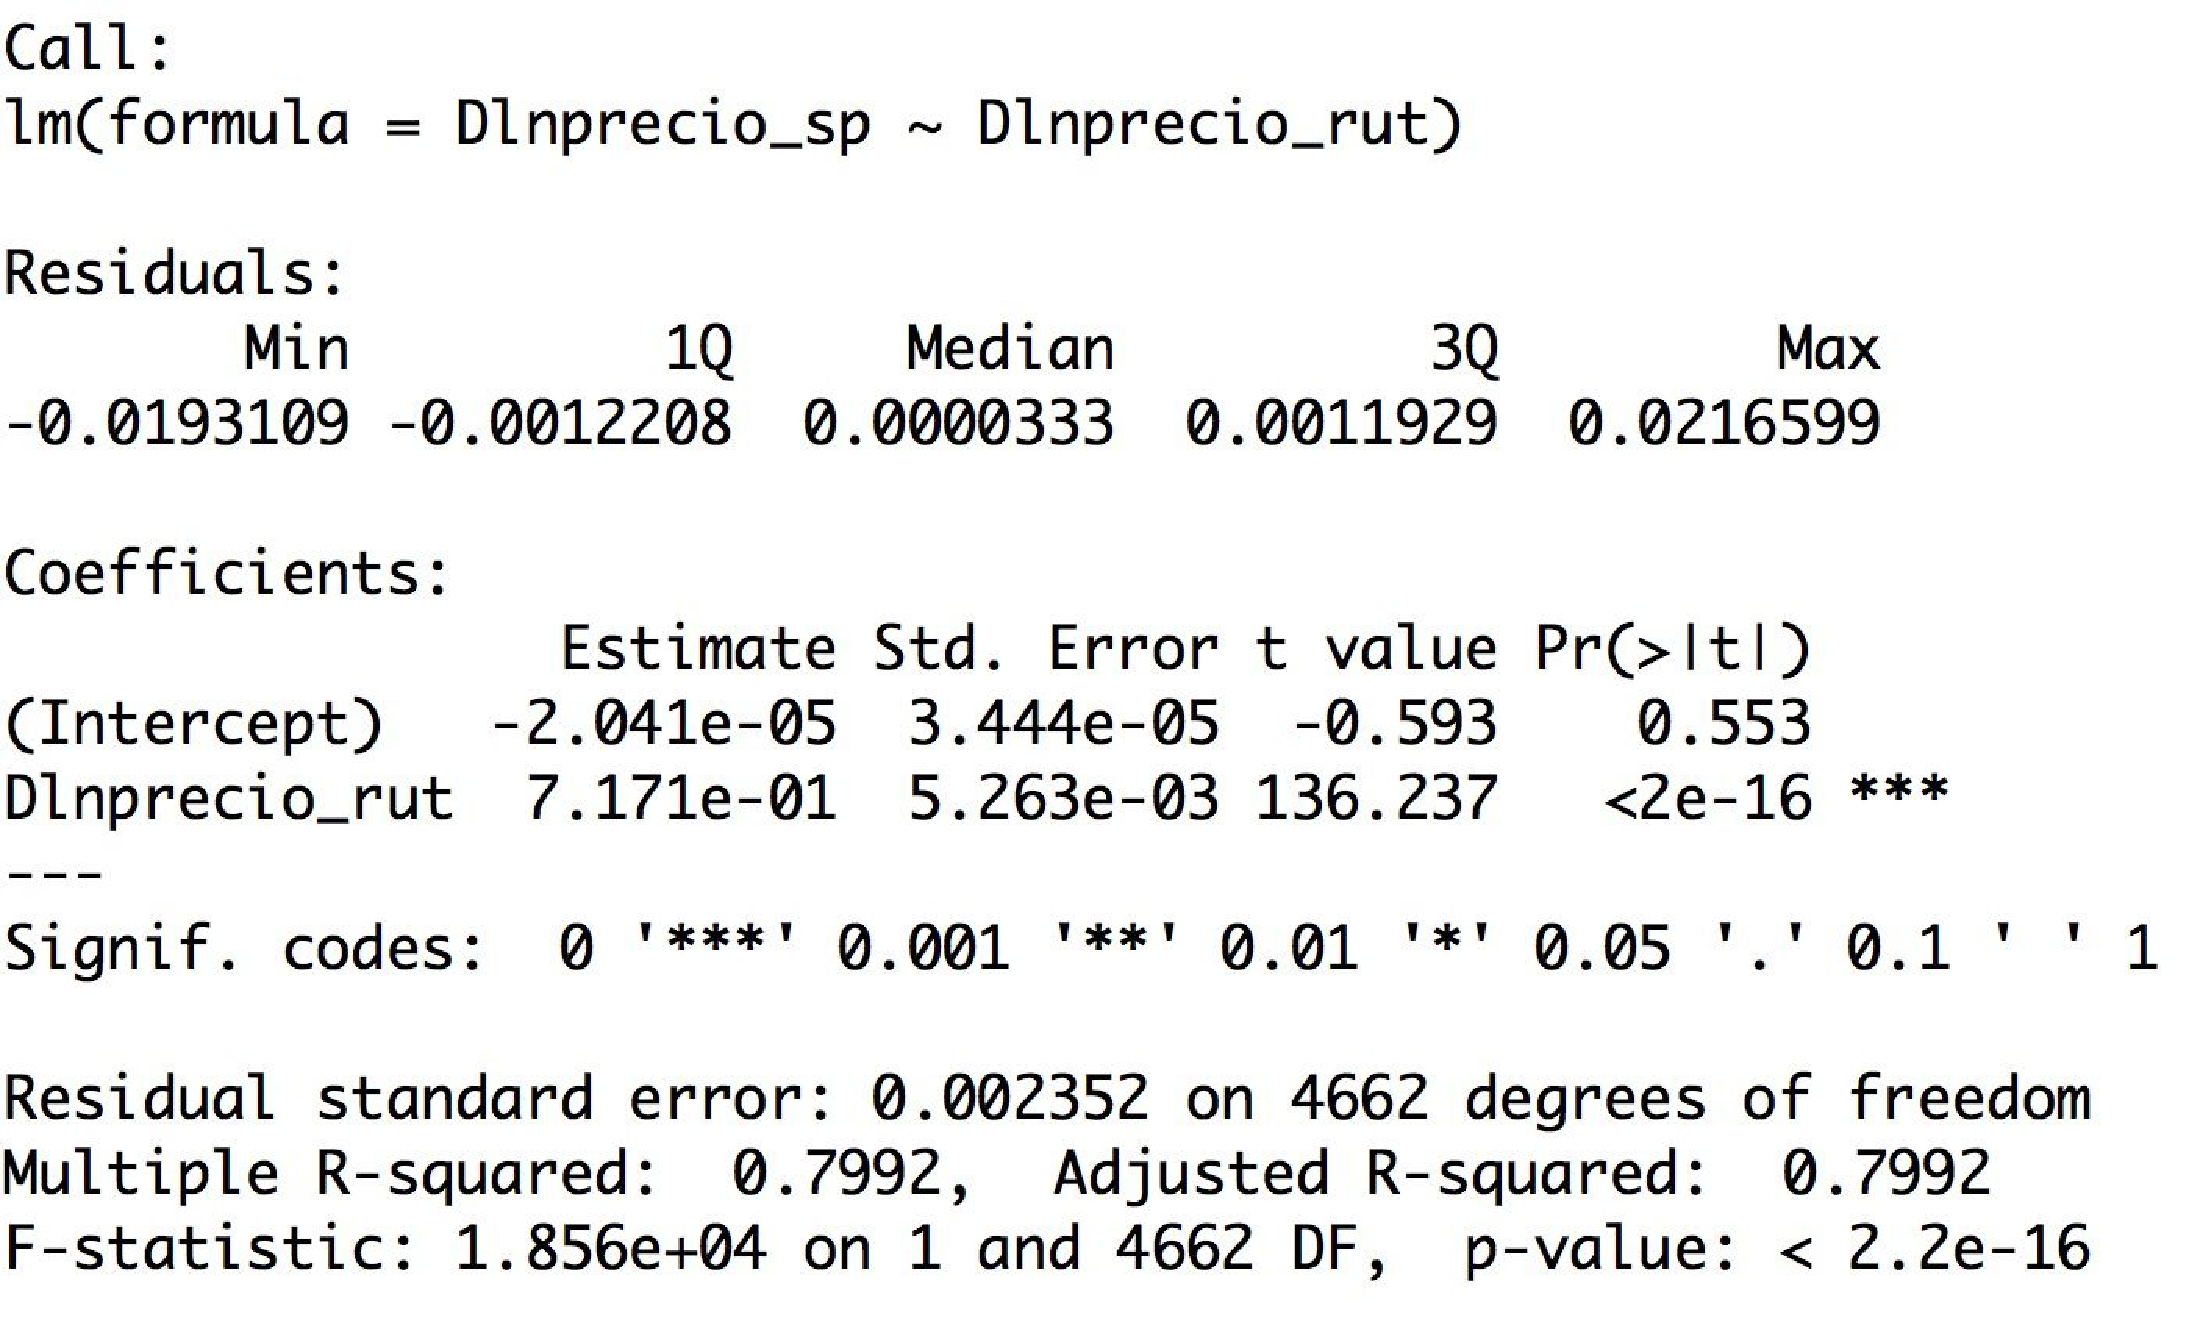
\includegraphics[width=\linewidth]{reg1.pdf}}
%	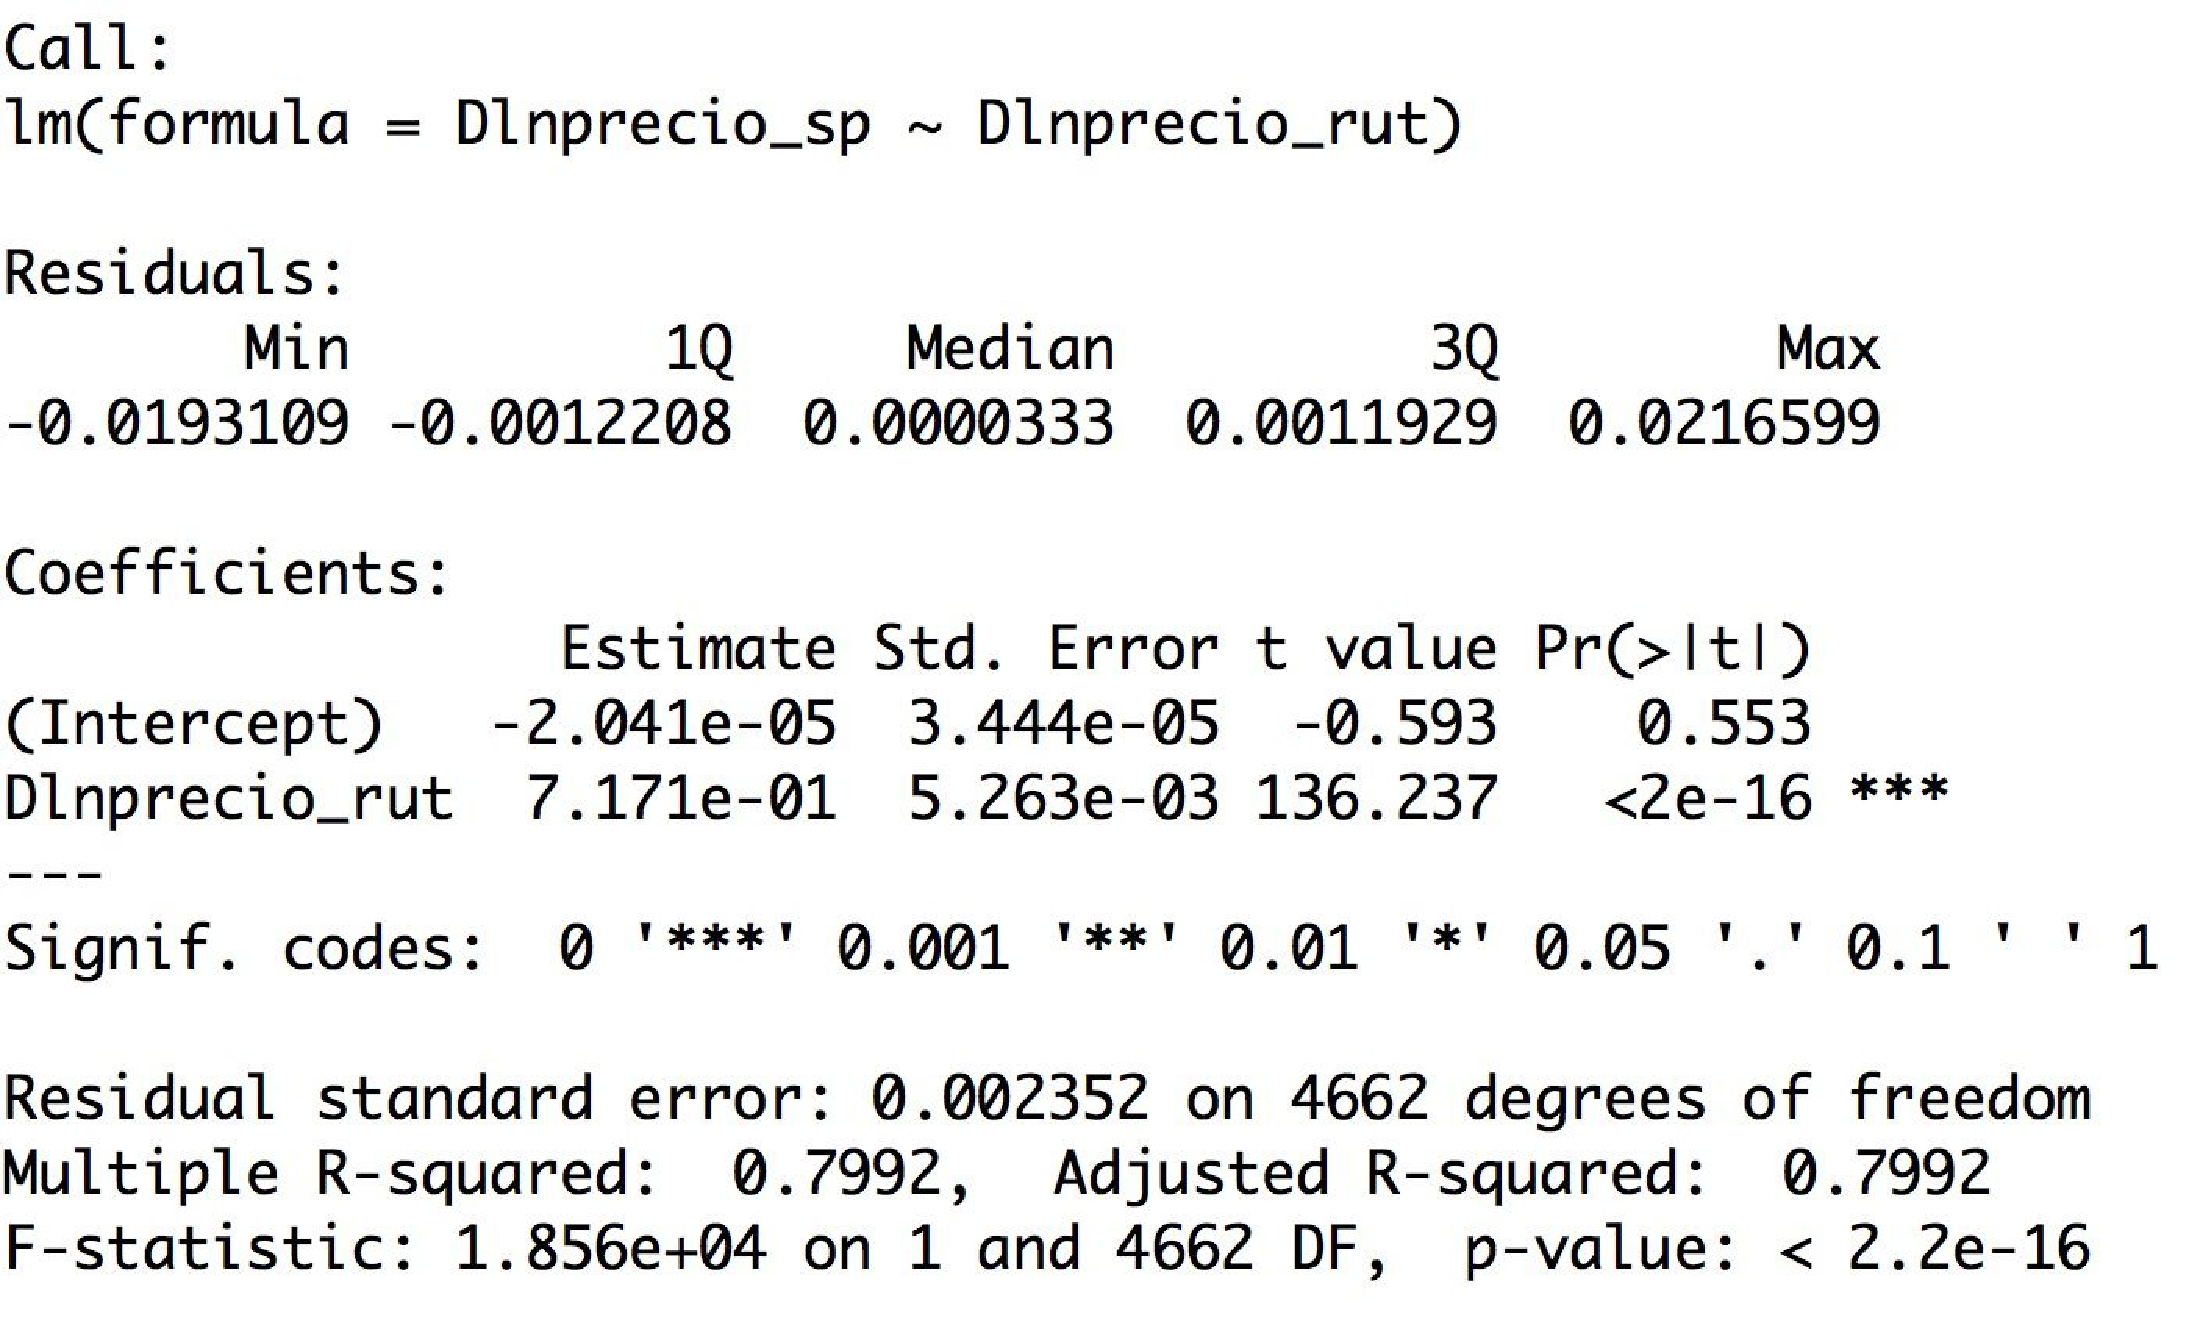
\includegraphics[scale=0.34]{reg1.pdf}
\end{figure}

%\end{frame}
%---------------------------------------------------------

%---------------------Slide 61 --------------------------
%\begin{frame}
%\frametitle{Ejemplo 3: Regresiones}
\lstset{caption = Código R para Regresiones,framexleftmargin=5mm, frame=shadowbox, rulesepcolor=\color{green}}
\begin{lstlisting}[title={‘Código R para Regresiones’},basicstyle=\ttfamily]{}
mydata1 <- read.csv("sp.csv", header=TRUE, 
					stringsAsFactors=FALSE)
precio_sp <- mydata1$"Adj.Close"; 
lnprecio_sp <- log10(precio_sp)
Dlnprecio_sp <- diff(lnprecio_sp ,1)
mydata2 <- read.csv("rut.csv", header= TRUE,
				stringsAsFactors = FALSE)
precio_rut <- mydata2$"Adj.Close" ; 
lnprecio_rut <- log10(precio_rut)
Dlnprecio_rut <- diff(lnprecio_rut ,1)
reg1 <- lm ( Dlnprecio_sp ~ Dlnprecio_rut)
summary(reg1)
\end{lstlisting}\label{ejemplo3Regresiones}
%
%\only<1|handout:1>{
%	\begin{exampleblock}{C\'odigo en R}
%		rm(list=ls())\\
%		mydata $<-$ read.csv (``/Users/marcelovillena/Desktop/sp.csv", header = TRUE, stringsAsFactors = FALSE)\\
%		$precio\_sp$ $<-$ mydata$\$$``Adj.Close" : $lnprecio\_sp$  $<-$ log10($precio\_sp$ ) ; $Dlnprecio\_sp$  $<-$ diff($lnprecio\_sp$ ,1)\\
%		mydata $<-$ read.csv (``/Users/marcelovillena/Desktop/rut.csv", header = TRUE, stringsAsFactors = FALSE)\\
%		$precio\_rut$ $<-$ mydata$\$$``rut" ; lnprecio\_rut  $<-$ log10($precio\_rut$ ) ; $Dlnprecio\_rut$  $<-$ diff($lnprecio\_rut$ ,1)\\
%		reg1 $<-$ lm ( $Dlnprecio\_sp$ $\string ~$ $Dlnprecio\_rut$)\\
%		summary(reg1)
%	\end{exampleblock}
%}
%\end{frame}
%---------------------Slide 62 --------------------------
%\begin{frame}
%\frametitle{Ejemplo 3: Regresioness}

\begin{figure}[H]
	\centering
	\textbf{Russell explicado por SP500}\par\medskip
	\fcolorbox{green}{blue}{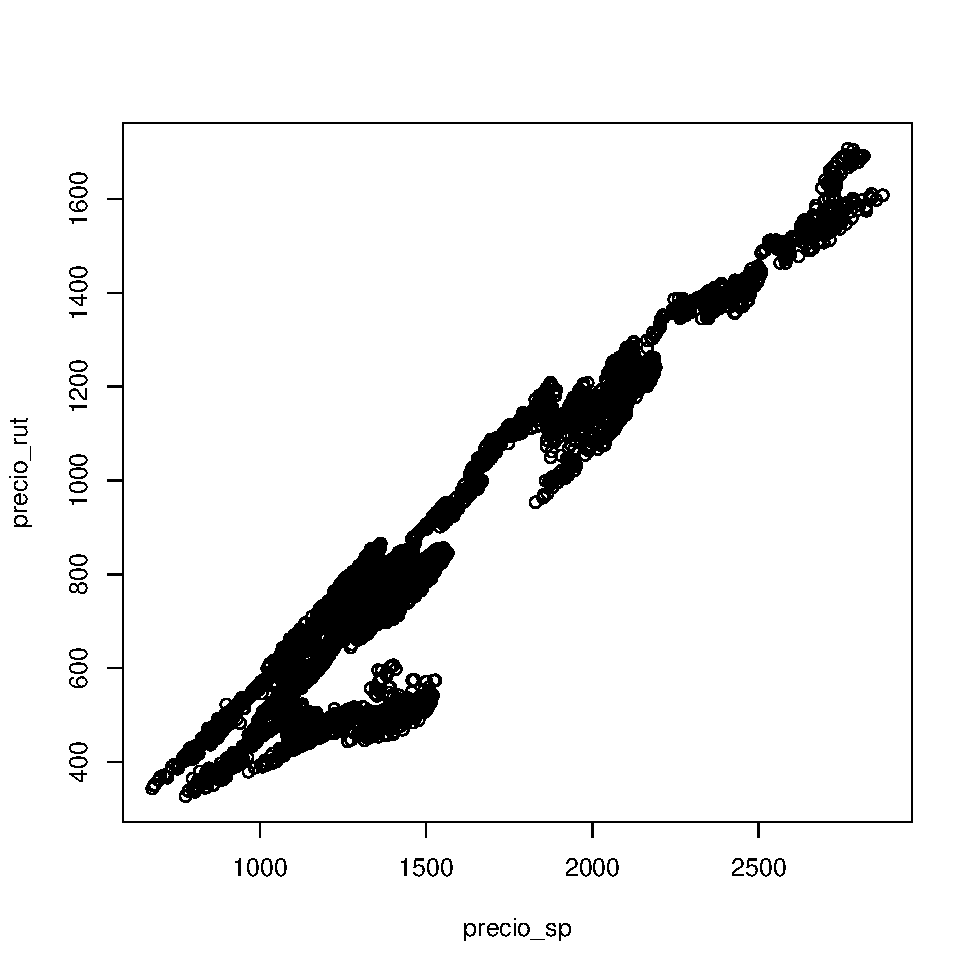
\includegraphics[width=\linewidth]{graph_precios.pdf}}
%	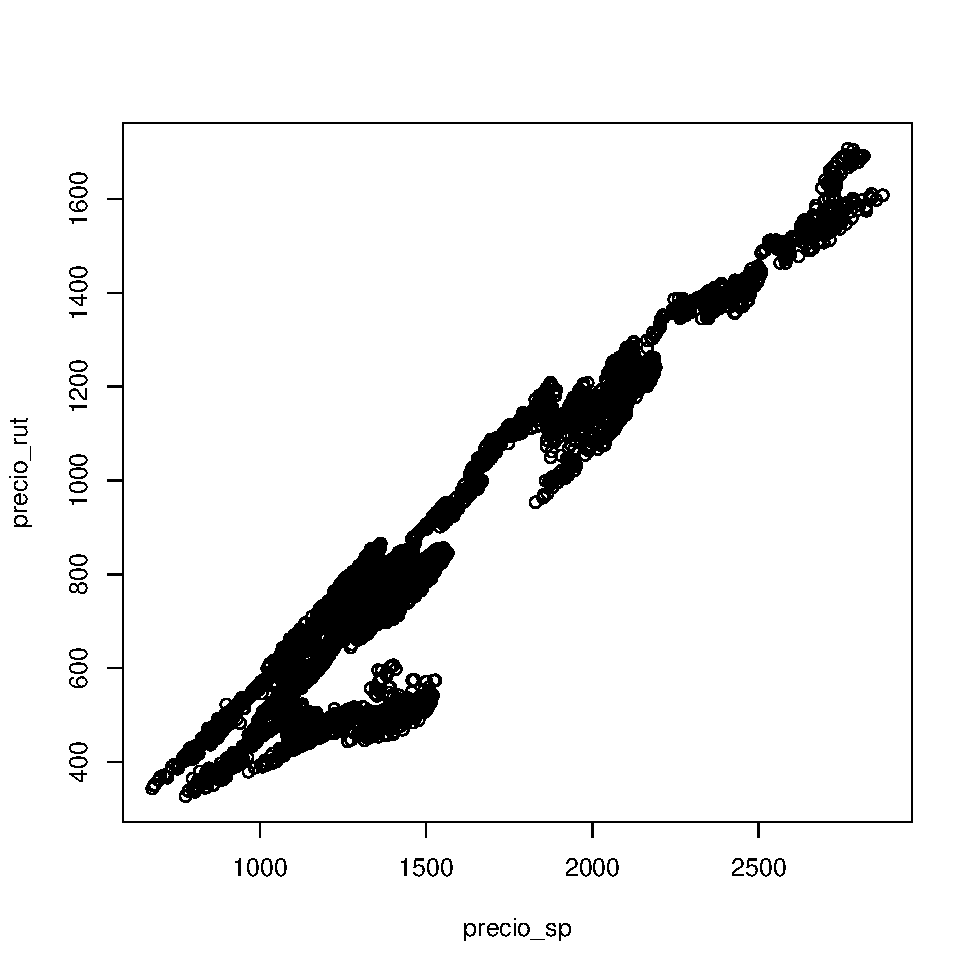
\includegraphics[scale=0.6]{graph_precios.pdf}
	\caption{Regresión de Russell 2000 en función del S\&P500}
\end{figure}

%\end{frame}

%---------------------------------------------------------	
%---------------------Slide 63 --------------------------
%\begin{frame}
%\frametitle{Ejemplo 3: Regresiones}

\pagebreak A partir del siguiente c\'odigo almacenamos los residuos y analizamos los supuestos que exige una buena regresi\'on.
\lstset{caption = Código R para Residuos,framexleftmargin=5mm, frame=shadowbox, rulesepcolor=\color{green}}
\begin{lstlisting}[title={‘Código R para Residuos de regresión’},basicstyle=\ttfamily]{}
residuos <- rstandard(reg1)
valores.ajustados <- fitted(reg1)
plot(valores.ajustados, residuos)
qqnorm(residuos)
qqline(residuos)
\end{lstlisting}\label{ejemplo3ResiduosRegresion}
%\only<1|handout:1>{
%	\begin{exampleblock}{C\'odigo en R}
%		residuos $<-$ rstandard(reg1)\\
%		valores.ajustados $<-$ fitted(reg1)\\
%		plot(valores.ajustados, residuos)\\
%		qqnorm(residuos)\\
%		qqline(residuos)\\
%	\end{exampleblock}
%}
%\end{frame}
%---------------------Slide 54 --------------------------
%\begin{frame}
%\frametitle{Ejemplo 3: Regresiones}



\begin{figure}[H]
	\centering
	\textbf{Homocedasticidad}\par\medskip
	\fcolorbox{green}{blue}{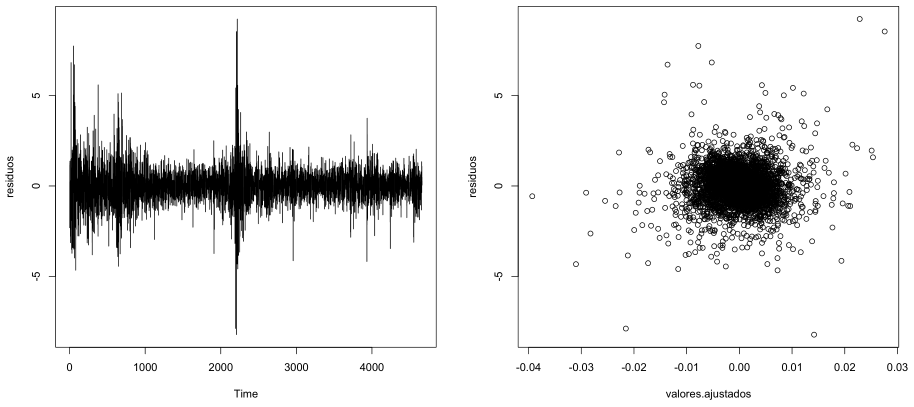
\includegraphics[width=\linewidth]{homocedasticidadD64.png}}
%	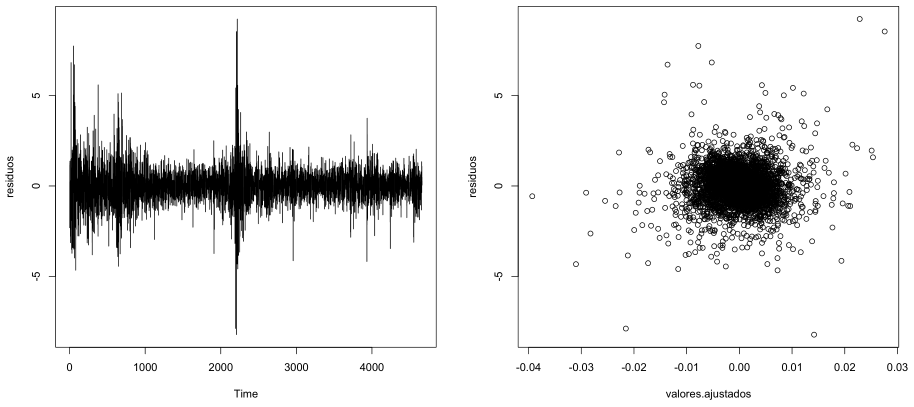
\includegraphics[scale=0.5]{homocedasticidadD64.png}

	\caption[Homocedasticidad]{Izquierda: Derecha}\label{fig11}
\end{figure}

%\end{frame}
%---------------------------------------------------------
%---------------------Slide 65 --------------------------
%\begin{frame}
%\frametitle{Ejemplo 3: Regresiones}



\begin{figure}[H]
	\centering
	\textbf{Normalidad de los residuos}\par\medskip
	\fcolorbox{green}{blue}{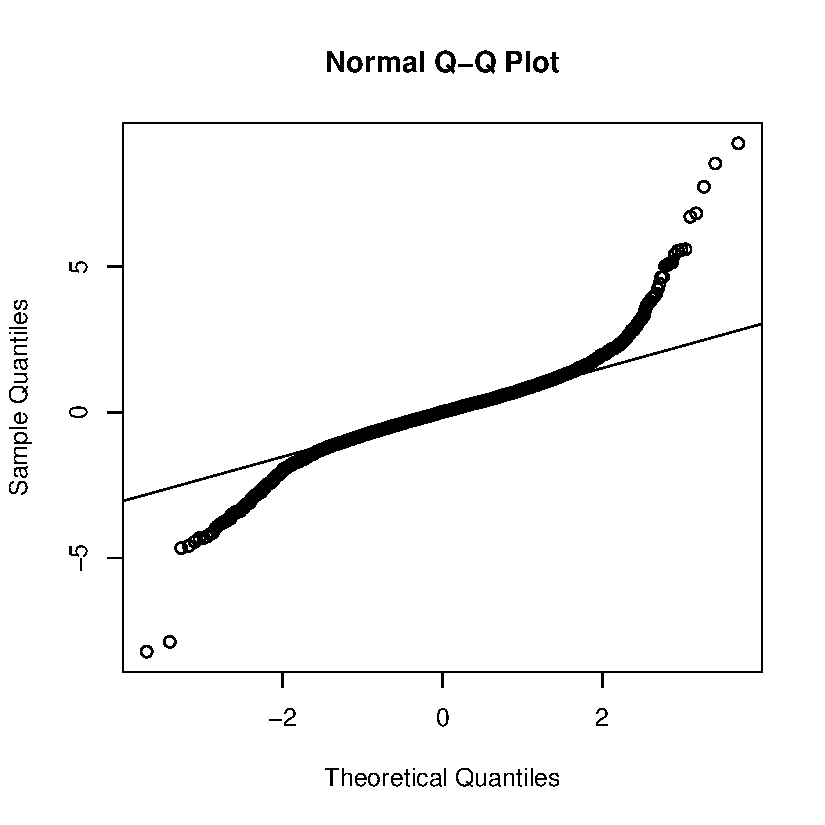
\includegraphics[width=\linewidth]{qqplot_reg1.pdf}}
	\caption{Grafico QQ-Plot de los residuos. La linea punteada indica el comportamiento de una distribución normal, mientras los puntos alejados de ella en los extremos dan cuenta de como se alejan los residuos del comportamiento normal.}
\end{figure}\label{fig12}

%\end{frame}
%\end{section}















%\section{Table}
%
%\begin{table}[htp]
%    \centering
%    \begin{tabular}{r|l|p{10cm}}
%        Right &  Left  &  Longlonglonglonglonglonglonglong longlonglonglonglonglonglonglonglonglonglonglonglong longlonglonglonglonglong \\
%        Right &  Left  &  Longlonglonglonglonglonglong
%        longlonglonglonglonglonglonglong
%        longlonglonglong
%        longlonglonglonglonglonglonglong 
%    \end{tabular}
%    \caption{This is a caption}
%    \label{tab:trans-sym}
%\end{table}
%
%\section{List}
%This is a List:
%\begin{itemize}
%    \item \textbf{Bullet 1}: Bullet 1 is bullet 1.
%    \item \textbf{Bullet 2}: Bullet 2 is bullet 2.
%\end{itemize}
%
%\section{Definition}
%\begin{definition}\label{def:def117}
%\textbf{DEFINITION NAME}: This is a definition.
%\end{definition} 
%
%% avoid bad break
%\vspace{5cm} 
%
%\section{Theorem}
%\begin{theo}[THEOREM NAME]{theo:theo1}
%This is a theorm. Below are equations.
%\begin{align}\label{eq:multi-equations}
%    \psi(\bvec{a}) &= A\cdot \bvec{a} + \bvec{t}.\\
%    R_x &=  \begin{bmatrix} 
%            0 & \cos(\theta) & -\sin(\theta)\\
%            0 & \sin(\theta) & \cos(\theta)\\
%            1 & 0 & 0
%         \end{bmatrix}, 
%    R_y =  \begin{bmatrix} 
%            \cos(\theta) & 0 & -\sin(\theta)\\
%            \sin(\theta) & 0 & \cos(\theta)\\
%            0 & 1 & 0
%         \end{bmatrix}, 
%    R_z =  \begin{bmatrix} 
%            \cos(\theta) & -\sin(\theta) & 0\\
%            \sin(\theta) & \cos(\theta) & 0 \\
%            0 & 0 & 1
%         \end{bmatrix} 
%\end{align}
%\end{theo}
%
%\begin{lem}[LEMMA NAME]{lem:leml}
%This is a lemma
%\end{lem}
%
%\begin{prf}[LEMMA NAME]{prf:leml}
%This is a proof.
%\end{prf}
%
%\section{Tikz Pictures}
%\begin{figure}[htp]
%    \centering
%        \begin{tikzpicture}[scale=0.6]
%            \draw[->] (0,-1)--(0,1.5)node[above] {$s$};
%            \draw[->] (-0.8,0.6) to[bend right] (0.8,0.6);
%            \draw[->] (0.9, 0.8)--(0.9, 1.2) node[right] {$\omega$};
%            \filldraw[dashed] (0,-0.2)--(0.9, -0.3) circle (1pt) node [right] {$q$};
%            \draw[->] (0.8, -0.9)--(1.2, -0.8) node[right] {$v$};
%        \end{tikzpicture}
%    \caption{This is a caption. }
%    \label{fig:rotation}
%\end{figure}

\curinstructor{Marcelo Villena Chamorro PhD.}
\chapter{Tópico II.- Univariate Time Series Models}

\section{Ejemplo de repaso clase anterior-Detrending global temperature}

Como vimos en la clase anterior, la evoluci\'on de la temperatura global manifestaba una tendencia lineal, por lo que podemos asumir que esta puede ser escrita como:
\begin{equation*} 
x_t =\mu_{t} + y_t
\end{equation*}
Veremos dos maneras de descomponer la serie, \textquotedblleft filtrando\textquotedblright \ la tendencia.

%---------------------------------------------------------
%---------------------Slide 4 --------------------------
%\begin{frame}
%\frametitle{Ejemplo de repaso clase anterior\newline
%	Detrending global temperature}

%\only<1|handout:1>{
%	\begin{exampleblock}{C\'odigo en R}
%		rm(list=ls())\\
%		mydata$<-$read.csv (``gtemp.csv")\\
%		gtemp$<-$mydata$\$$``gtem"\\
%		plot(gtemp, type=``o", ylab= ``Global Temperature Deviations'')\\
%		t$<-$1:142\\
%		summary(reg $<-$ lm(gtemp $\string ~$ t))\\
%		plot(gtemp, type=``o", ylab=``Global Temperature Deviations'')\\
%		abline(reg)\\
%	\end{exampleblock}
%}
\lstset{caption=Ejemplo 1 Sacando la tendencia de la serie temperatura global,framexleftmargin=5mm, frame=shadowbox, rulesepcolor=\color{green}}
\begin{lstlisting}[title={‘Código R: ejemplo 1 Obtención de la componente \textquotedblleft tendencia\textquotedblright de la serie temperatura global(gtemp).’},basicstyle=\ttfamily]{}
rm(list=ls())
mydata<-read.csv ("gtemp.csv")
gtemp<-mydata$"gtem"
plot(gtemp, type="o", ylab="Global Temperature Deviations")
t<-1:142
summary(reg <- lm(gtemp ~ t))
plot(gtemp, type="o", ylab="Global Temperature Deviations")
abline(reg)
\end{lstlisting}
%\end{frame}

%---------------------------------------------------------
%---------------------Slide 5--------------------------
%\begin{frame}
%\frametitle{Ejemplo de repaso clase anterior\newline

\begin{figure}[H]
	\centering
	\textbf{Ejemplo 1: Detrending global temperature}\par\medskip
	\fcolorbox{green}{blue}{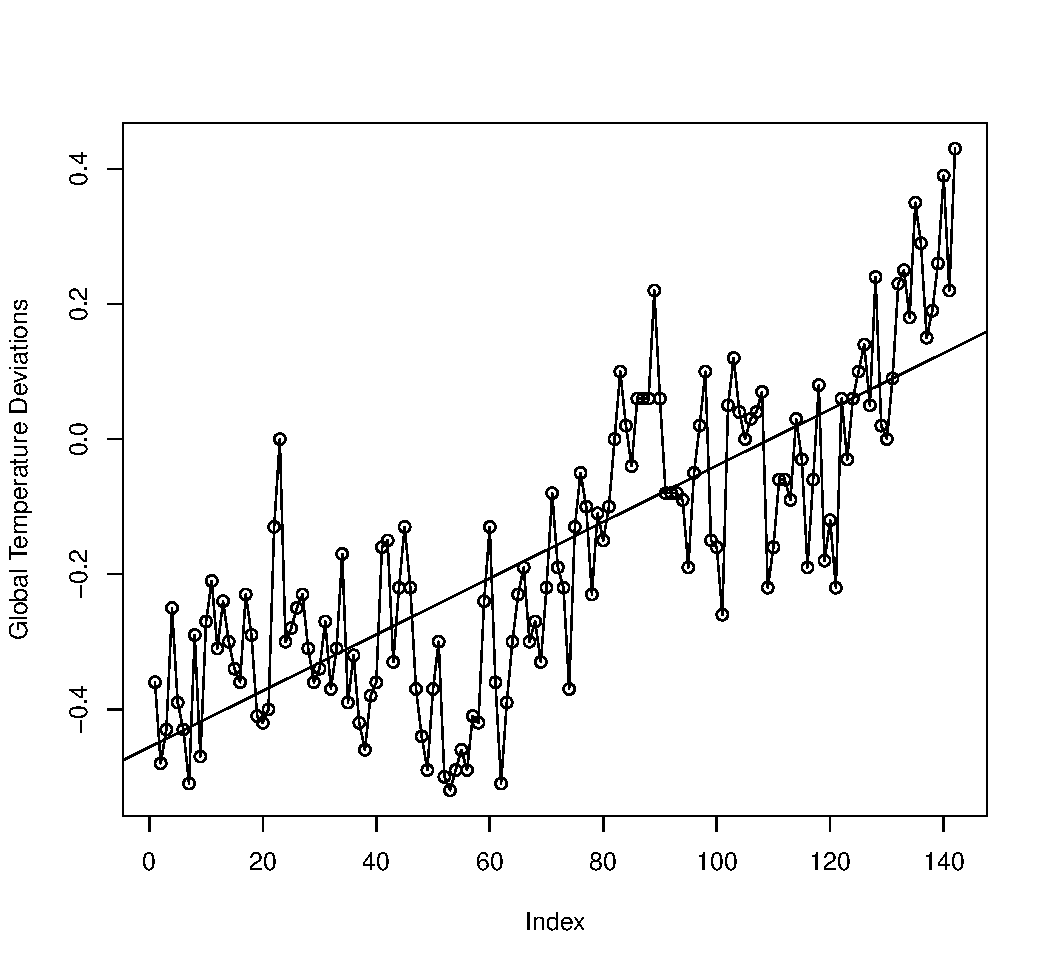
\includegraphics[width=\linewidth,scale=0.5]{gtemp_graph.pdf}}
	\caption{La figura muestra en línea punteada la tendencia de la serie de tiempo.}\label{fig1}
\end{figure}

%\end{frame}
%---------------------------------------------------------
%---------------------Slide 6--------------------------
%\begin{frame}
%\frametitle{Ejemplo de repaso clase anterior\newline
%	Detrending global temperature}

\begin{figure}[H]
	\centering
	\textbf{Detrending global temperature}\par\medskip
	\fcolorbox{green}{blue}{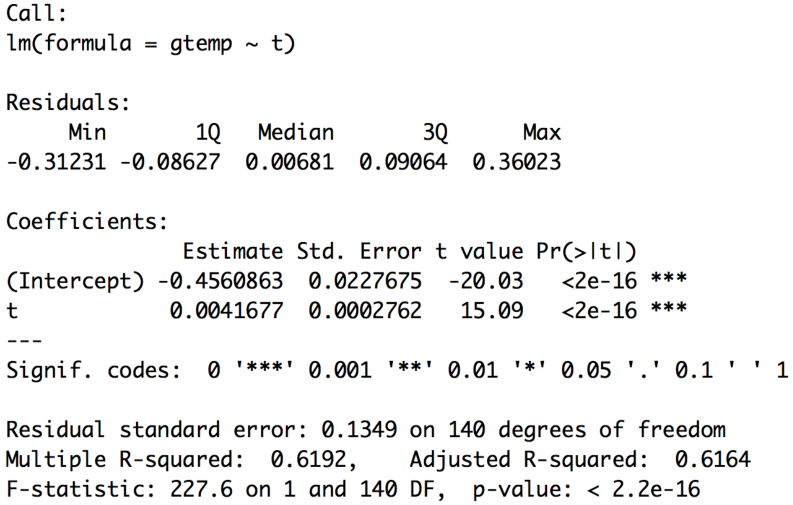
\includegraphics[width=\linewidth,scale=0.5]{reg_ej1.png}}
	\caption{Parametría de la regresión de temperatura en el tiempo.}\label{fig2}
\end{figure}

%\end{frame}
%---------------------------------------------------------
%---------------------Slide 7 --------------------------
%\begin{frame}
%\frametitle{Ejemplo de repaso clase anterior\newline
%	Detrending global temperature}

%\only<1|handout:1>{
%	\begin{exampleblock}{C\'odigo en R}
%		reg1= lm(gtemp$\string ~$ time(gtemp), na.action=NULL) \\
%		par(mfrow=c(2,1))\\
%		plot(resid(reg1), type=``o", main=``detrended")\\
%		plot(diff(gtemp), type=``o", main=``first difference")\\
%	\end{exampleblock}
%}
\lstset{caption=Ejemplo 1 Detrending global temperature,framexleftmargin=5mm, frame=shadowbox, rulesepcolor=\color{green}}
\begin{lstlisting}[title={‘Código R: ejemplo 1 Regresando gtemp sobre tiempo.’},basicstyle=\ttfamily]{}
reg1= lm(gtemp~time(gtemp), na.action=NULL) 
par(mfrow=c(2,1))
plot(resid(reg1), type="o", main="detrended")
plot(diff(gtemp), type="o", main="first difference")
\end{lstlisting}
%\end{frame}
%=================================
%---------------------Slide 8--------------------------
%\begin{frame}
%\frametitle{Ejemplo de repaso clase anterior\newline
%	Detrending global temperature}

\begin{figure}[H]
	\centering
	\textbf{Ejemplo 1: Detrending global temperature}\par\medskip
	\fcolorbox{green}{blue}{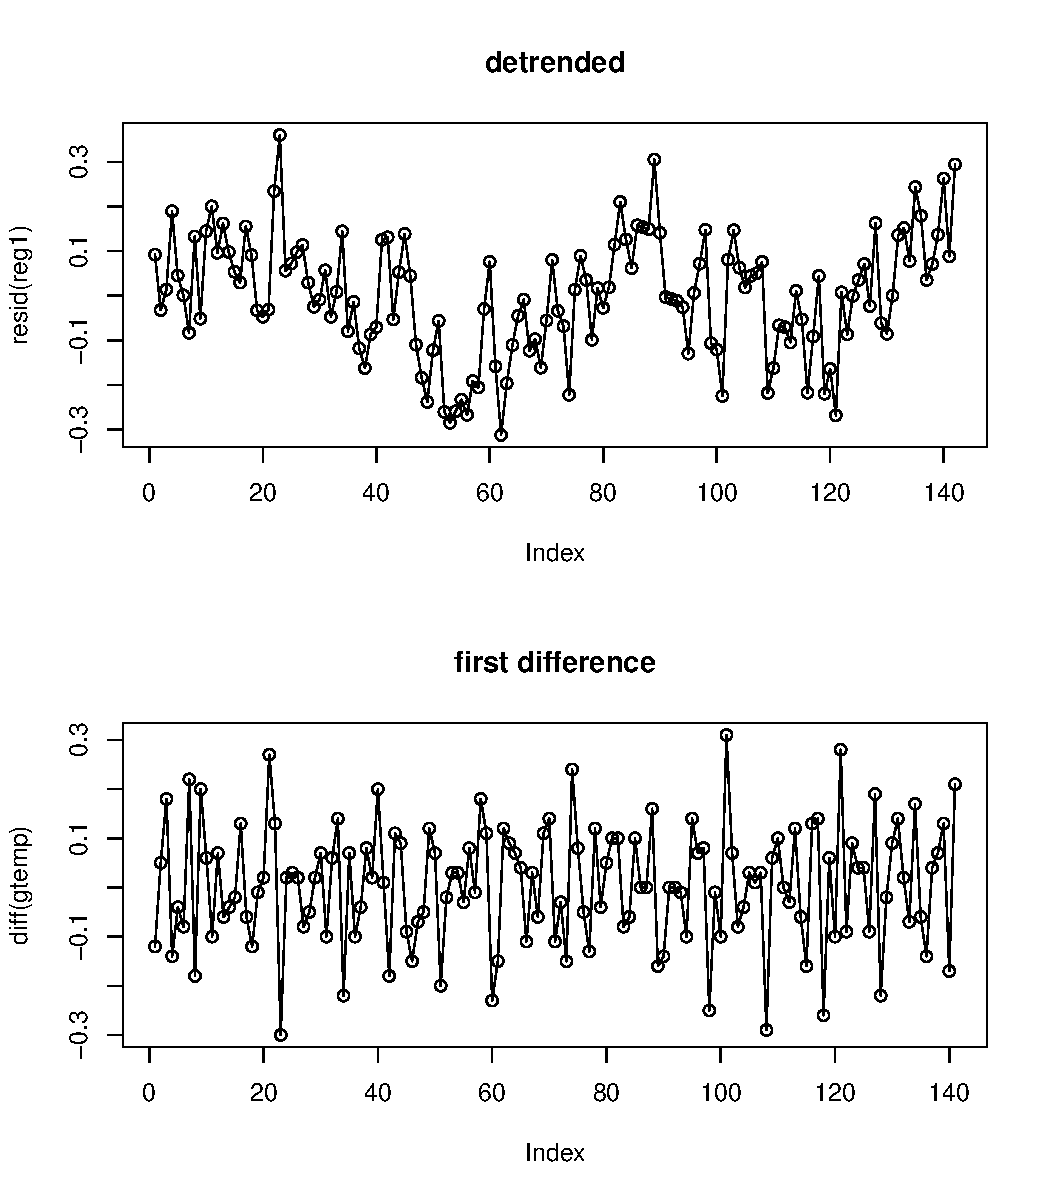
\includegraphics[width=\linewidth,scale=0.5]{detrended.pdf}}
	\caption{Arriba: residuos de la regresión. Abajo:primeras diferencias de la serie original}\label{fig3}
\end{figure}

%\begin{figure}[p]
%	\centering
%	\textbf{Detrending global temperature}\par\medskip
%	\fcolorbox{red}{yellow}{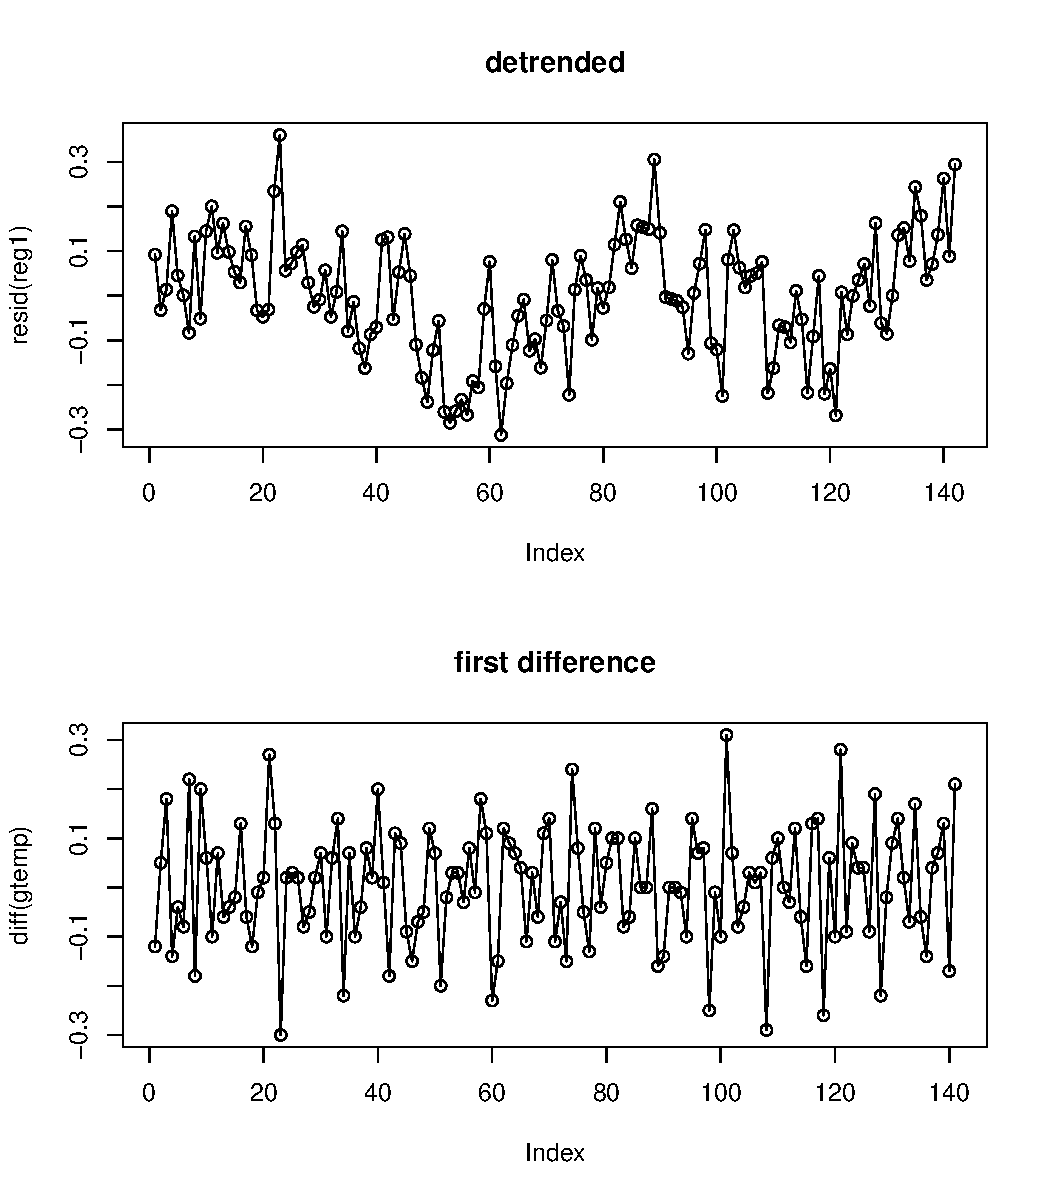
\includegraphics[width=\linewidth,scale=0.5]{detrended.pdf}}
%	\caption{Arriba: residuos de la regresión. Abajo:primeras diferencias de la serie original}\label{fig3.2}
%\end{figure}

%\end{frame}

%---------------------------------------------------------
%---------------------Slide 9 --------------------------
%\begin{frame}
%\frametitle{Ejemplo de repaso clase anterior\newline
%Detrending global temperature}

%\only<1|handout:1>{
%\begin{exampleblock}{C\'odigo en R}
%	par(mfrow=c(3,1)) \\
%	acf(gtemp, 48, main=``gtemp")\\
%	acf(resid(reg), 48, main=``detrended")\\
%	acf(diff(gtemp), 48, main=``first difference")\\
%\end{exampleblock}
%}
\lstset{caption=Ejemplo 1 Detrending global temperature,framexleftmargin=5mm, frame=shadowbox, rulesepcolor=\color{green}}
\begin{lstlisting}[title={‘Código R: ejemplo 1 Correlogramas de series.’},basicstyle=\ttfamily]{}
par(mfrow=c(3,1)) # plot ACFs
acf(gtemp, 48, main="gtemp")
acf(resid(reg), 48, main="detrended")
acf(diff(gtemp), 48, main="first difference")
\end{lstlisting}

%\end{frame}
%---------------------------------------------------------
%---------------------Slide 10--------------------------
%\begin{frame}
%\frametitle{Ejemplo de repaso clase anterior\newline
%Detrending global temperature}

\begin{figure}[H]
	\centering
	\textbf{Ejemplo 1: Autocorrelograma}\par\medskip
	\fcolorbox{green}{blue}{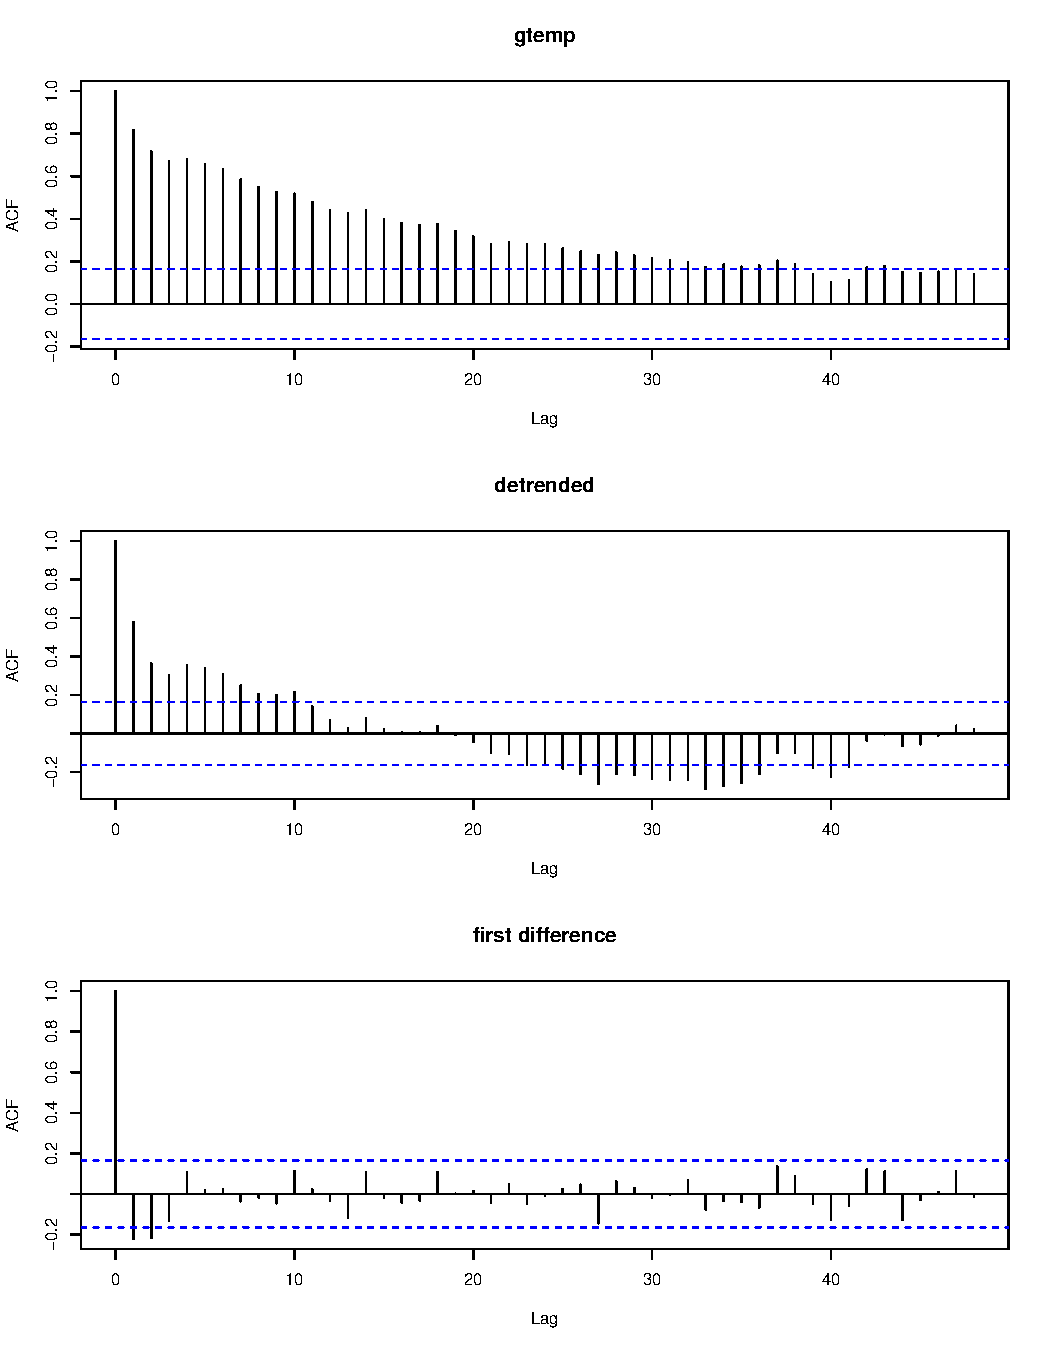
\includegraphics[width=\linewidth,scale=0.5]{acf_example1.pdf}}
	\caption{Autocorrelogramas para diferentes retardos(lags): Arriba:serie original. Medio: residuos de la regresión. Abajo: primera diferencia de la serie original}\label{fig4}
\end{figure}

%\end{frame}
%---------------------------------------------------------
%---------------------Slide 11--------------------------
%\begin{frame}
%\frametitle{Sobre la descomposici\'on de una serie}
\pagebreak\section{Sobre la descomposici\'on de una serie}

En los gr\'aficos podemos apreciar que la primera diferencia de la serie produce resultados diferentes a la eliminaci\'on de la tendencia mediante la regresi\'on de la tendencia.\\
En el caso de los gr\'aficos ACF, el proceso diferenciado muestra una autocorrelaci\'on mi\'{\i}nima, lo que puede implicar que la serie de temperatura global es similar una caminata aleatoria con deriva.\\
Es interesante notar que si la serie es una caminata aleatoria con deriva, la media de la serie diferenciada, que es una estimaci\'on de la deriva, es aproximadamente $,0066$, pero con un gran error est\'andar:\\
%\only<1|handout:1>{
%	\begin{exampleblock}{C\'odigo en R}
%		mean (diff (gtemp))\\
%		sd (diff (gtemp)) / sqrt (longitud (diff (gtemp)))
%	\end{exampleblock}
%}
\lstset{caption=Ejemplo 1 Detrending global temperature,framexleftmargin=5mm, frame=shadowbox, rulesepcolor=\color{green}}
\begin{lstlisting}[title={‘Código R: ejemplo 1: sobre la descomposición de una serie - media y error estandar’},basicstyle=\ttfamily]{}
mean (diff(gtemp)) #media
sd (diff (gtemp)) / sqrt (length(diff (gtemp))) #error estandar
\end{lstlisting}
%\end{frame}
%---------------------------------------------------------
%---------------------Slide 12--------------------------

%\begin{frame}
%\frametitle{Sobre la descomposici\'on de una serie}

Una ventaja de diferenciar sobre la estimaci\'on de una tendencia,  para eliminar las tendencias, es que no se estiman par\'ametros en la operaci\'on de diferenciaci\'on. Una desventaja, sin embargo, es que la diferenciaci\'on no arroja una estimaci\'on del proceso estacionario $y_t$.\\
%\vspace{5mm}	 
De esta forma, si una estimaci\'on de $y_t$ es esencial, entonces la estimación de una tendencia puede ser la forma más apropiada para eliminar las tendencias de la serie. Si el objetivo es forzar los datos a la estacionaridad, entonces la diferenciaci\'on puede ser m\'as apropiada. La diferenciaci\'on tambi\'en es una herramienta viable si la tendencia es fija.\\
%\vspace{3mm}	
En EE.UU. el procedimiento oficial de descomposici\'on y ajuste estacional se llama:\\
%\vspace{3mm}	
\textbf{X-13-ARIMA (http://www.census.gov/srd/www/x13as/)}

%\end{frame}

%---------------------------------------------------------
%---------------------Slide 13--------------------------

%\begin{section}{Procesos no estacionarios, integrados y el test de ra\'{\i}z unitaria}
\pagebreak\section{Procesos no estacionarios, integrados y el test de ra\'{\i}z unitaria}
%\begin{frame}
%\frametitle{Procesos no estacionarios, integrados y el test de ra\'{\i}z unitaria}

Recordemos que si una serie de tiempo es estacionaria, su media, su varianza y su autocovarianza (en diferentes rezagos) permanecen iguales sin importar el momento del tiempo en el cual se midan; es decir, son \textbf{invariantes respecto al tiempo}.
\par
Por otro lado, hemos visto que la estacionaridad es una caracter\'{\i}stica deseable, por ejemplo, en t\'erminos de la normalidad de las variables. Sin embargo, en la pr\'actica nos encontramos con:
\par
%\only<1->{
\begin{itemize}
	\item[(i)] Procesos No-estacionarios: Cuando un proceso estoc\'astico de series de tiempo es dependiente del tiempo.
	\item[(ii)] Procesos Integrados: un proceso no-estacionario, el cual puede ser transformado a proceso estacionario diferenciando.
\end{itemize}
%}

%\end{frame}

%---------------------------------------------------------
%---------------------Slide 14--------------------------
%\begin{frame}
%\frametitle{Procesos Integrados}
\subsection{Procesos Integrados}

Con respecto a los Procesos Integrados, partimos definiendo:
%\only<1->{
	\begin{itemize}
		\item La secuencia $\{x_t\}$ es integrada de orden $d$, $I(d)$, si esta requiere ser diferenciada $d$ veces para llegar a ser estacionaria.
		\item Todos los \textbf{Procesos Integrados son no-estacionarios}, pero no todos los procesos no-estacionarios son integrados.
		\item Si la secuencia $\{x_t\}$  tiene una ra\'{\i}z unitaria, entonces, es un proceso integrado, y de aqu\'{\i} no-estacionario.
	\end{itemize}
%}
%
%\end{frame}

%---------------------------------------------------------
%---------------------Slide 15--------------------------
%\begin{frame}
%\frametitle{Consecuencias de los Procesos Integrados (Ra\'{\i}z Unitaria)}
\subsection{Consecuencias de los Procesos Integrados (Ra\'{\i}z Unitaria)}
%\only<1->{
\begin{itemize}
	\item Es importante se\~nalar que los test estad\'{\i}sticos est\'andares no son apropiados cuando los MCO (OLS) son aplicados a procesos integrados, ver por ejemplo \cite{granger1974spurious}.
	\item Si la secuencia $\{x_t\}$ es un proceso de ra\'{\i}z unitaria, entonces, cualquier shock tiene un efecto permanente (que no decae). De aqu\'{\i}, la serie de tiempo es modelada apropiadamente suponiendo una tendencia estoc\'astica. La serie de tiempo entonces puede ser definida como estacionaria diferenciable, y se le deber\'a sacar la tendencia diferenciando. 
	\item En este contexto, \textbf{los t\'erminos no-estacionariedad, caminata aleatoria, ra\'{\i}z unitaria y tendencia estoc\'astica se consideran sin\'onimos}. 
\end{itemize}
%}
%
%\end{frame}

%---------------------------------------------------------
%---------------------Slide 16--------------------------
%\begin{frame}
%\frametitle{Test de Ra\'{\i}z Unitaria}
\subsection{Test de Ra\'{\i}z Unitaria}
Considere el siguiente proceso autoregresivo:

\begin{equation} \label{AR1}
x_t =\alpha_1 x_{t-1} + \epsilon_t
\end{equation}

Si $\alpha_1=1$, la secuencia $x_t$ es una ra\'{\i}z unitaria.

El test est\'andar para probar esta hip\'otesis, consiste en restar $x_{t-1}$ a la ecuaci\'on anterior de forma que:

\begin{equation}
\triangle x_t =\gamma x_{t-1} + \epsilon_t
\end{equation}

donde $\gamma=\alpha_1-1$, y $\triangle x_t = x_t - x_{t-1}$. En este contexto, probar la hip\'otesis que la ecuaci\'on (1) tiene una ra\'{\i}z unitaria, $\alpha_1 = 1$, es equivalente a probar la hip\'otesis de $\gamma=0$ en ecuaci\'on (2). 
Este es b\'asicamente el enfoque de Dickey-Fuller (DF) para ra\'{\i}ces unitarias, ver por ejemplo \cite{dickey1981likelihood}. Adicionalmente existe el test aumentado de Dickey-Fuller (ADF), y muchos otros tests que se basan el l\'ogicas similares, y que utilizaremos durante el curso.

%\end{frame}

%---------------------------------------------------------
%---------------------Slide 17 --------------------------
%\begin{frame}
%\frametitle{Ejemplo de Test de Ra\'{\i}z Unitaria - Dickey-Fuller}
\subsubsection{Ejemplo de Test de Ra\'{\i}z Unitaria - Dickey-Fuller}
%\only<1|handout:1>{
%\begin{exampleblock}{C\'odigo en R}
%install.packages(``tseries")\\
%library(tseries)\\
%adf.test(gtemp)\\
%adf.test(resid(reg1))\\
%adf.test(diff(gtemp))\\
%\end{exampleblock}
%}
\lstset{caption=Ejemplo ,framexleftmargin=5mm, frame=shadowbox, rulesepcolor=\color{green}}
\begin{lstlisting}[title={‘Código R: Ejemplo Test de Raíz Unitaria - Dickey-Fuller ’},basicstyle=\ttfamily]{}
library(tseries)
adf.test(gtemp)
adf.test(resid(reg1))
adf.test(diff(gtemp))
\end{lstlisting}
%\end{frame}
%---------------------------------------------------------
%---------------------Slide 18 --------------------------
%\begin{frame}
%\frametitle{Ejemplo de Test de Ra\'{\i}z Unitaria - Dickey-Fuller}
%\begin{mdframed}[style=MyFrame]
%Augmented Dickey-Fuller Test\\
%data:  gtemp\\
%Dickey-Fuller = -2.0624, Lag order = 5, p-value =
%0.5505\\
%alternative hypothesis: stationary\\
%\vspace{5mm}	    
%Augmented Dickey-Fuller Test\\
%data:  resid(reg1)\\
%Dickey-Fuller = -2.0624, Lag order = 5, p-value =
%0.5505\\
%alternative hypothesis: stationary\\
%\vspace{5mm}	    
%Augmented Dickey-Fuller Test\\
%data:  diff(gtemp)\\
%Dickey-Fuller = -6.8179, Lag order = 5, p-value = 0.01\\
%alternative hypothesis: stationary\\
%\end{mdframed}

\begin{figure}[H]
	\centering
	\textbf{Ejemplo: Resultados de Test de Raíz Unitaria - Dickey-Fuller}\par\medskip
	\fcolorbox{green}{blue}{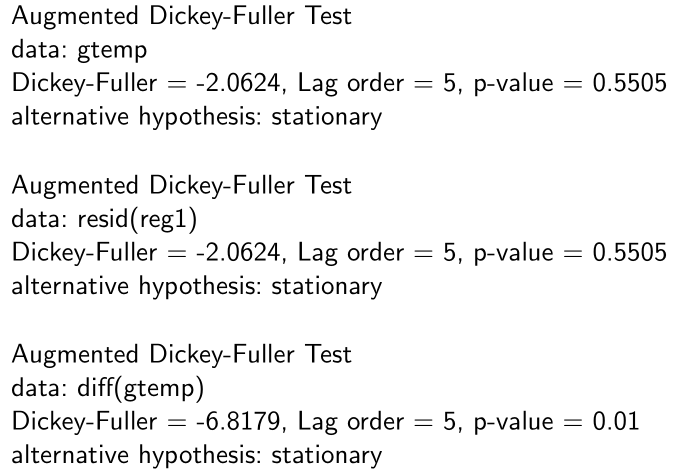
\includegraphics[width=\linewidth,scale=0.5]{adf_ejRaizUnitaria.png}}
	\caption{Test de raíz unitaria Dickey-Füller para diferentes series: Arriba:serie original (gtemp). Medio: residuos de la regresión(resid(reg1)). Abajo: primera diferencia de la serie original (diff(gtemp))}\label{fig5}
\end{figure}
%\end{frame}
%
%\end{section}
%---------------------------------------------------------
%---------------------Slide 19--------------------------
%\begin{section}{Modelos ARIMA: modelando el corto plazo}
%\begin{frame}
%\frametitle{Modelos ARIMA: modelando el corto plazo}
\pagebreak\section{Modelos ARIMA: modelando el corto plazo}

En el a\~no 1970, la metodolog\'{\i}a propuesta por George Box y Gwilym Jenkins, \cite{BoxJenkins} , dos ingenieros con formaci\'on estad\'{\i}stica sistematizan modelos estad\'{\i}sticos para el an\'alisis de series temporales univariantes, teniendo en cuenta para esto la dependencia existente entre los datos. \\
As\'{\i}, cada observaci\'on es modelada en funci\'on de los valores anteriores, la variable tiempo, por tanto, juega un papel fundamental. 

%\end{frame}

%---------------------------------------------------------
%---------------------Slide 20--------------------------
%\begin{frame}
%\frametitle{Modelos ARIMA: modelando el corto plazo}


Los modelos de predicci\'on de Box-Jenkins pertenecen a la familia de modelos alg\'ebraicos lineales, que consideran que una serie temporal real constituye una probable realizaci\'on de un determinado proceso estoc\'astico.\\
\vspace{4mm}	
Estos modelos se conocen con el nombre gen\'erico de ARIMA (Auto-regresive Integrated Moving Average), el cual deriva de sus tres componentes Autoregresivo (AR), Integrado (I) de Medias M\'oviles (MA). Modelar una serie temporal supone identificar un modelo ARIMA adecuado que se ajuste a la serie objeto de estudio, debe contener los m\'{\i}nimos elementos necesarios para describir el fen\'omeno y ser \'util para realizar previsiones.

%\end{frame}
%---------------------------------------------------------
%---------------------Slide 21--------------------------
%\begin{frame}
%\frametitle{Sobre el operador de retroceso - backshift operator}
\subsection{Sobre el operador de retroceso - backshift operator}
\begin{mdframed}[style=MyFrame]
\begin{definition}\label{def}
	\textbf{Definici\'on: operador de retroceso (backshift operator):}
		\begin{equation}
		B x_t = x_{t-1} 
		\end{equation}
		\begin{equation}
		B^2 x_t =  B(B x_t) = B x_{t-1} = x_{t-2}
		\end{equation}
		As\'{\i}:
		\begin{equation}
		B^k x_t = x_{t-k} 
		\end{equation} 
\end{definition}
\end{mdframed}

%\only<1|handout:1>{
%	\begin{block}{Definici\'on: operador de retroceso (backshift operator) }
%		Definimos el operador de retroceso (backshift operator) como:
%		
%		\begin{equation}
%		B x_t = x_{t-1} 
%		\end{equation}
%		\begin{equation}
%		B^2 x_t =  B(B x_t) = B x_{t-1} = x_{t-2}
%		\end{equation}
%		As\'{\i}:
%		\begin{equation}
%		B^k x_t = x_{t-k} 
%		\end{equation}
%	\end{block}
%}

De esta forma tenemos que la primera diferencia se puede definir en t\'erminos de lags, en otras palabras del operador de retroceso:
\begin{equation}
\triangle x_t = x_t - x_{t-1}= (1 - B) x_t 
\end{equation}
En general:
\begin{equation}
\triangle^d x_t = (1 - B)^d x_t 
\end{equation}

%\end{frame}
%---------------------------------------------------------
%---------------------Slide 22--------------------------
%\begin{frame}
%\frametitle{Modelos ARIMA: modelando el corto plazo}
\begin{mdframed}[style=MyFrame]
\begin{definition}\label{def2}
	\textbf{Definici\'on:  $AR (p)$:}
	Un modelo autorregresivo de orden p, frecuentemente abreviado como $AR(p)$, tiene la forma:
	\begin{equation}
	x_t = \phi_1 x_{t-1} +  \phi_2 x_{t-2} + \dots{} +  \phi_p x_{t-p} + \epsilon_t
	\label{ar}
	\end{equation}
	donde $x_t$ es una serie estacionaria, y  $\phi_1$,  $\phi_2$,  \dots{} , $\phi_p$ son constantes. 
	Si la media de $x_t$ es $\mu$, entonces podemos reemplazar $x_t-\mu$ en $\eqref{ar}$
	\begin{equation}
	x_t-\mu = \phi_1 (x_{t-1}-\mu) +  \phi_2 (x_{t-2}-\mu) + \dots{} +  \phi_p (x_{t-p}-\mu) + \epsilon_t
	\end{equation}
	\begin{equation}
	x_t = \alpha + \phi_1 x_{t-1} +  \phi_2 x_{t-2} + \dots{} +  \phi_p x_{t-p} + \epsilon_t
	\end{equation}
	donde $\alpha = \mu(1-\phi_1-\phi_2\dots{}\phi_p)$\\
	Usando los operadores de retroceso $AR(p)$ queda como:
	\begin{equation}
	(1- \phi_1 B + \phi_2 B^2 - \dots{}  - \phi_p B^p )
	\end{equation}
	o incluso m\'as concisamente
	\begin{equation}
	\phi (B) x_t = \epsilon_t
	\end{equation}	
\end{definition}
\end{mdframed}

%\only<1|handout:1>{
%\begin{block}{Definici\'on: $AR (p)$}
%	Un modelo autorregresivo de orden p, frecuentemente abreviado como $AR(p)$, tiene la forma:
%	\begin{equation}
%	x_t = \phi_1 x_{t-1} +  \phi_2 x_{t-2} + \dots{} +  \phi_p x_{t-p} + \epsilon_t
%	\label{ar}
%	\end{equation}
%	donde $x_t$ es una serie estacionaria, y  $\phi_1$,  $\phi_2$,  \dots{} , $\phi_p$ son constantes. 
%	Si la media de $x_t$ es $\mu$, entonces podemos reemplazar $x_t-\mu$ en $\eqref{ar}$
%	\begin{equation}
%	x_t-\mu = \phi_1 (x_{t-1}-\mu) +  \phi_2 (x_{t-2}-\mu) + \dots{} +  \phi_p (x_{t-p}-\mu) + \epsilon_t
%	\end{equation}
%	\begin{equation}
%	x_t = \alpha + \phi_1 x_{t-1} +  \phi_2 x_{t-2} + \dots{} +  \phi_p x_{t-p} + \epsilon_t
%	\end{equation}
%	donde $\alpha = \mu(1-\phi_1-\phi_2\dots{}\phi_p)$\\
%	Usando los operadores de retroceso $AR(p)$ queda como:
%	\begin{equation}
%	(1- \phi_1 B + \phi_2 B^2 - \dots{}  - \phi_p B^p )
%	\end{equation}
%	o incluso m\'as concisamente
%	\begin{equation}
%	\phi (B) x_t = \epsilon_t
%	\end{equation}
%\end{block}
%}

%\end{frame}

%---------------------------------------------------------
%---------------------Slide 23--------------------------
%\begin{frame}
%\frametitle{Ejemplo Proceso Autoregresivo de Orden 1: AR(1)}
\subsection{Ejemplo Proceso Autoregresivo de Orden 1: AR(1)}

En un procesos AR(1) la variable $x_t$ queda \'unicamente por su valor pasado $x_{t-1}$:
\begin{equation}
x_t = \phi x_{t-1} + \epsilon_t
\end{equation}

donde como sabemos $\epsilon_t$ es un proceso de ruido blanco con media cero y varianza constante $\sigma^2$, y $\phi$ es un par\'ametro. Para verificar que el modelo AR(1) es estacionario debemos probar que es:\\
\vspace{4mm}	
\textbf{(1) Estacionario en media}
\begin{equation}
E(x_t) = E(\phi x_{t-1} + \epsilon_t)=\phi E(x_{t-1} )
\end{equation}
Para que el proceso sea estacionario, la media debe ser constante y finita en el tiempo, lo que implica:
\begin{equation}
E(x_t) = \phi E(x_{t} )
E(x_t) = \frac{0}{1-\phi}=0
\end{equation}
\\
Por lo tanto, para que el proceso sea estacionario el par\'ametro $\phi \ne 0$.

%\end{frame}

%---------------------------------------------------------
%---------------------Slide 24--------------------------
%\begin{frame}
%\frametitle{Ejemplo Proceso Autoregresivo de Orden 1: AR(1)}

\textbf{(2) Estacionario en covarianza}

Para verificar que el modelo AR(1) sea estacionario, la varianza debe ser constante y finita en el tiempo:

\begin{equation}
\gamma = E(x_t-E(x_t))^2 = E(\phi x_{t-1} + \epsilon_t - 0)^2 = \phi^2 var(x_{t-1}) + \sigma^2
\end{equation}

Asumiendo que el proceso es estacionario:
\begin{equation}
E(x_t)^2 = var(x_{t-1}) = var(x_{t}) = \gamma
\end{equation}
De aqu\'{\i} tenemos que:

\begin{equation}
\gamma  = \phi^2 \gamma + \sigma^2
\end{equation}

Por lo que:
\begin{equation}
\gamma  = \frac{\sigma^2}{1-\phi^2}
\end{equation}\\
Para que un proceso sea estacionario, varianza constante y finita, es necesario que $|\phi|< 1$.
%\end{frame}

%---------------------------------------------------------
%---------------------Slide 25--------------------------
%\begin{frame}
%\frametitle{Ejemplo Proceso Autoregresivo de Orden 1: AR(1)}

Si se cumple que $|\phi|< 1$, entonces podemos representar el modelo AR(1) como un proceso lineal dado por:

\begin{equation}
x_t = \sum_{j=0}^{\infty} \phi^j \epsilon_{t-j}
\label{causal}
\end{equation}

La ecuaci\'on $\eqref{causal}$ se llama \textbf{soluci\'on estacionaria causal del modelo}. El t\'ermino causal se refiere al hecho de que $x_t$ no depende del futuro. De hecho, por simple sustituci\'on,\\
\begin{equation}
\underbrace{\sum_{j=0}^{\infty} \phi^j\epsilon_{t-j}}_{x_t} = \underbrace{\phi\left(\sum_{k=0}^{\infty} \phi^k\epsilon_{t-1-k}\right)}_{x_{t-1}}+\epsilon_t
\end{equation}

%\end{frame}

%---------------------------------------------------------
%---------------------Slide 26 --------------------------
%\begin{frame}
%\frametitle{Simulaci\'on modelo AR(1) }
\subsection{Simulaci\'on modelo AR(1)}

%\only<1|handout:1>{
%	\begin{exampleblock}{C\'odigo en R}
%		par(mar=c(1,1,1,1))\\
%		par(mfrow=c(2,1))\\
%		plot(arima.sim(list(order=c(1,0,0), ar=.9), n=100), ylab=``x",\\
%		main=(expression(AR(1)~~~phi==+.9)))\\
%		plot(arima.sim(list(order=c(1,0,0), ar=-.9), n=100), ylab=``x",\\
%		main=(expression(AR(1)~~~phi==-.9)))\\
%	\end{exampleblock}
%}
\lstset{caption=Ejemplo ,framexleftmargin=5mm, frame=shadowbox, rulesepcolor=\color{green}}
\begin{lstlisting}[title={‘Código R: Simulaci\'on modelo AR(1) ’},basicstyle=\ttfamily]{}
par(mar=c(1,1,1,1))
par(mfrow=c(2,1))
plot(arima.sim(list(order=c(1,0,0), ar=.9), n=100), ylab="x",
main=(expression(AR(1)~~~phi==+.9)))

plot(arima.sim(list(order=c(1,0,0), ar=-.9), n=100), ylab="x",
main=(expression(AR(1)~~~phi==-.9)))
\end{lstlisting}
%\end{frame}
%---------------------------------------------------------
%---------------------Slide 27 --------------------------
%\begin{frame}
%\frametitle{Simulaci\'on modelo AR(1) }

\begin{figure}[H]
	\centering
	\textbf{Simulación AR(1)}\par\medskip
	\fcolorbox{green}{blue}{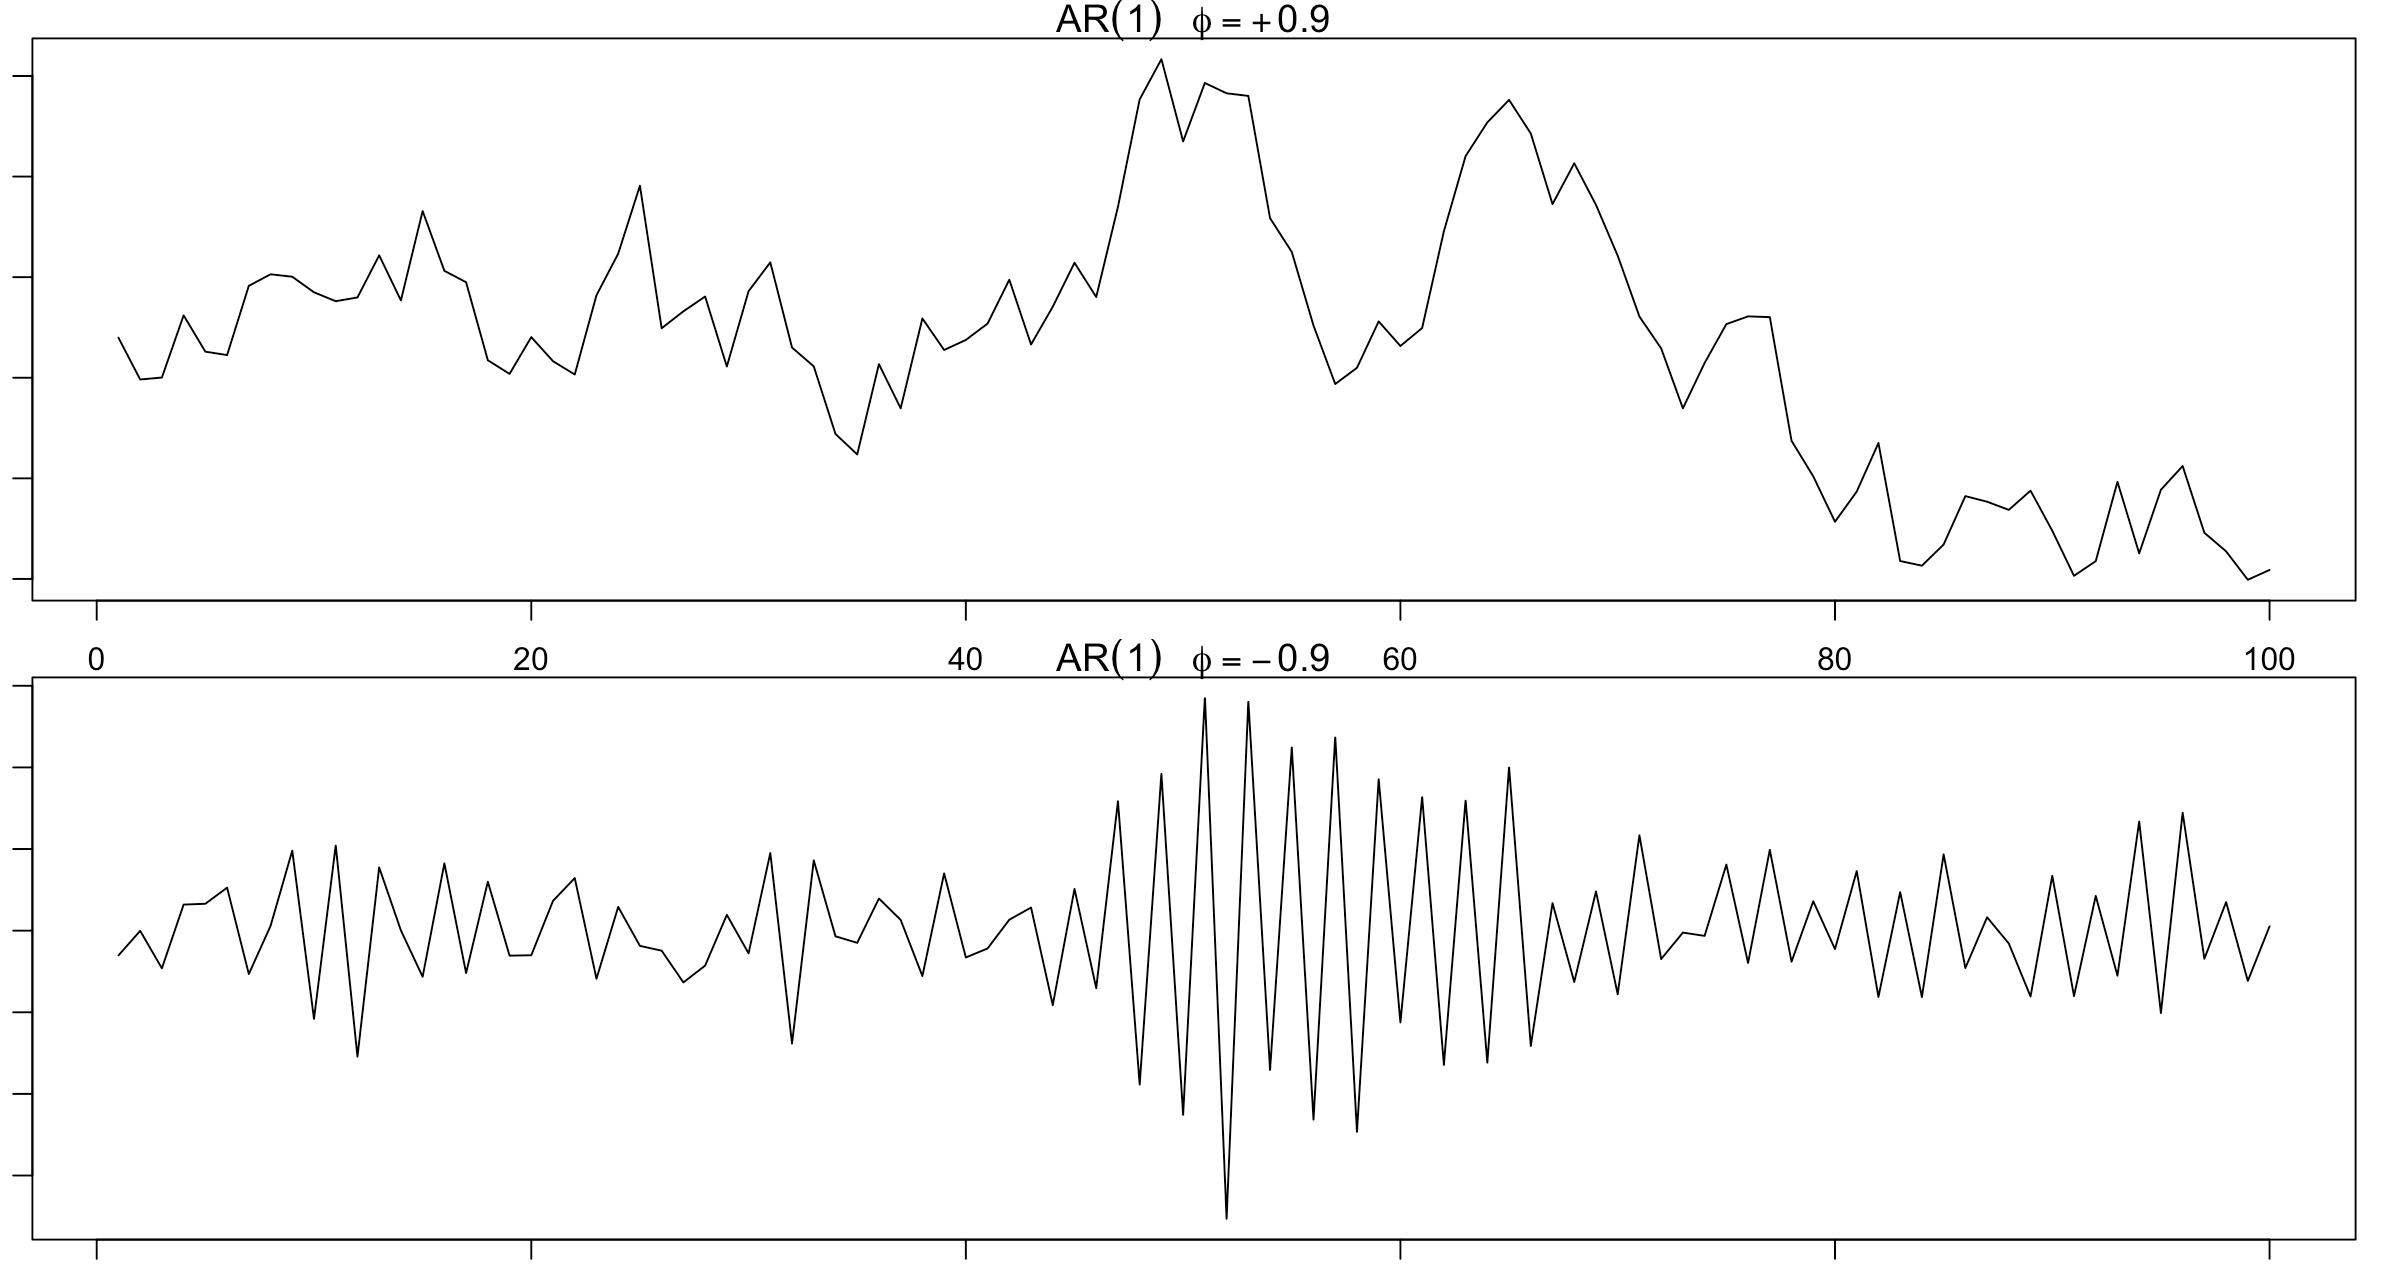
\includegraphics[width=\linewidth]{ar.png}}
	\caption{Simulaciones procesos AR(1): Arriba:$\phi=+0.9$.  Abajo: $\phi=-0.9$}\label{fig6}
\end{figure}

%\end{frame}

%---------------------------------------------------------
%---------------------Slide 28--------------------------
%\begin{frame}
%\frametitle{Identificaci\'on modelo AR(1) }
\subsection{Identificaci\'on modelo AR(1)}

Para el caso de un proceso del tipo AR, el correlograma, representaci\'on gr\'afica de la funci\'on de autocorrelaci\'on, tendr\'a un
comportamiento amortiguado hacia cero con todos los valores positivos, en caso de que $\theta > 0$, o bien alternando el signo, comenzando con negativo, si  $\theta < 0$.

\begin{figure}[H]
	\centering
	\textbf{Proceso Autoregresivo: AR(1)}\par\medskip
	\fcolorbox{green}{blue}{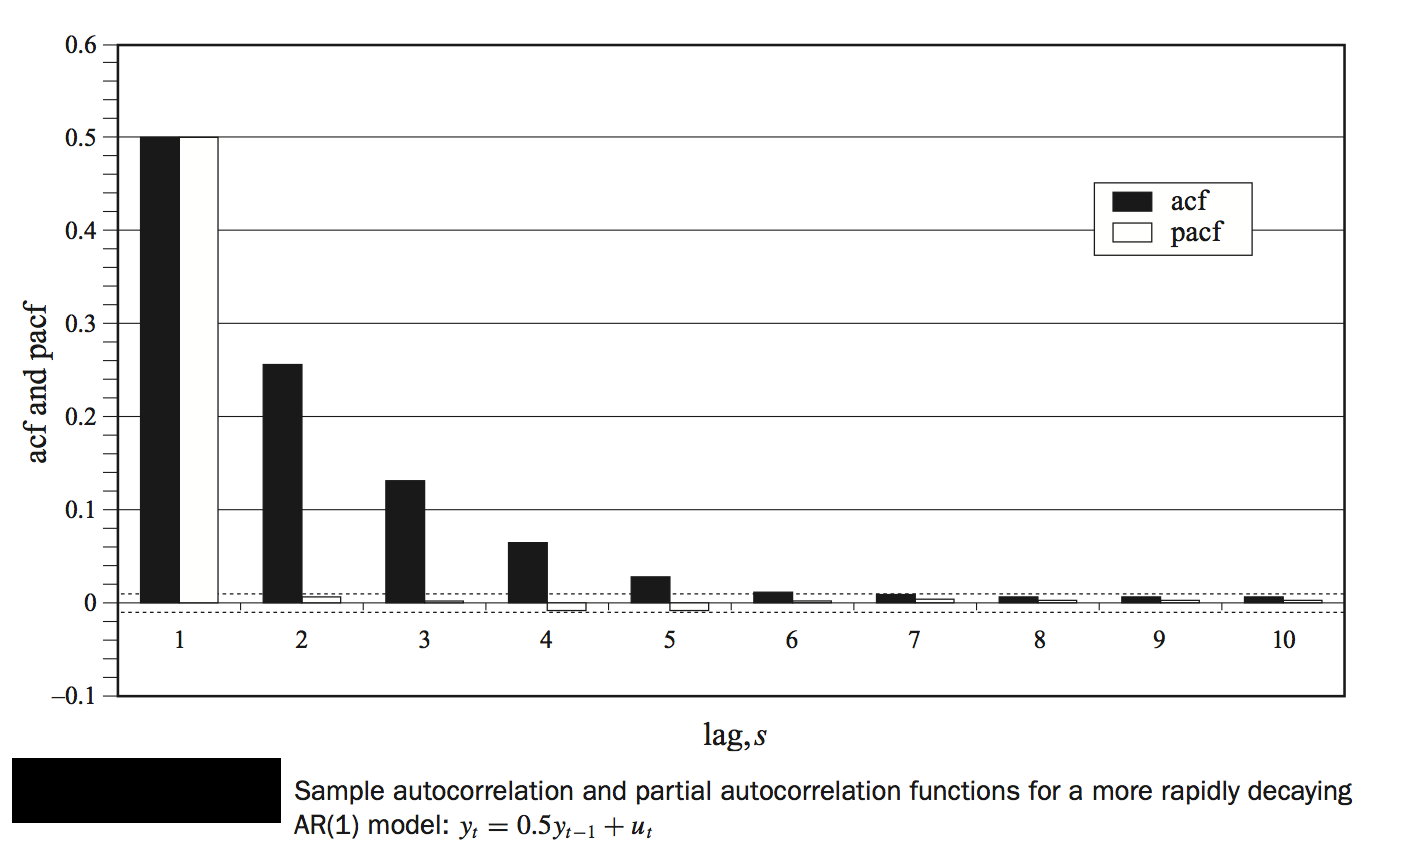
\includegraphics[width=\linewidth]{ar1corr.png}}
	\caption{Autocorrelogramas para autocorrelación(acf) y autocorrelación parcial(pacf)}\label{fig7}
\end{figure}


%\end{frame}
%---------------------------------------------------------
%---------------------Slide 29--------------------------
%\begin{frame}
%\frametitle{Identificaci\'on modelo AR(1) }

\begin{figure}[H]
		\centering
		\textbf{Proceso Autoregresivo: AR(1)}\par\medskip
		\fcolorbox{green}{blue}{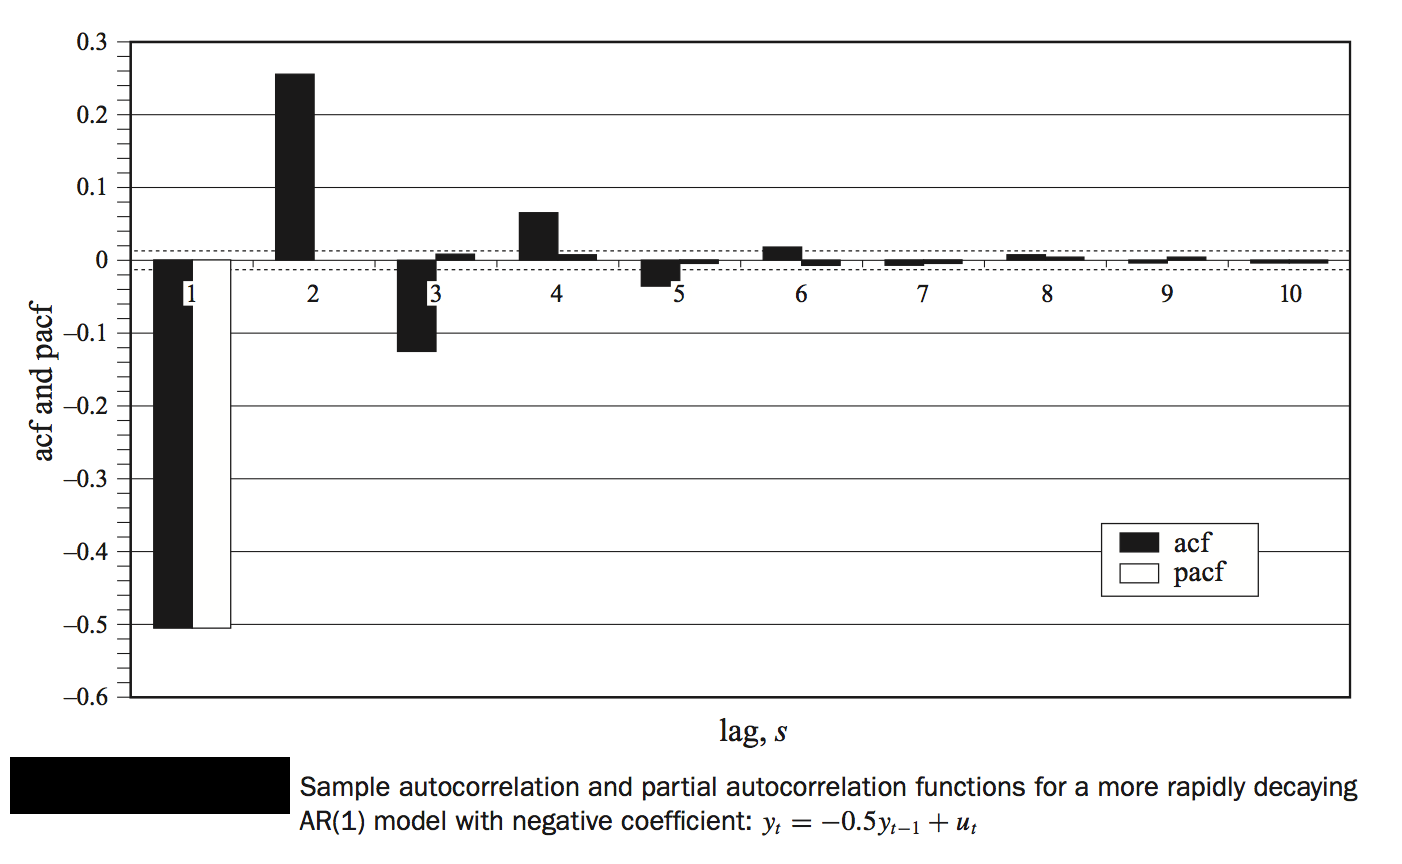
\includegraphics[width=\linewidth]{ar1corrb.png}}
		\caption{Autocorrelogramas para autocorrelación(acf) y autocorrelación parcial(pacf)}\label{fig8}

\end{figure}

%\end{frame}
%---------------------------------------------------------
%---------------------Slide 30--------------------------
%\begin{frame}
%\frametitle{Modelos ARIMA: modelando el corto plazo}

%\textbf{Media M\'ovil - MA (q)}
\pagebreak
\subsection{Media M\'ovil - MA (q)}

Como una alternativa a la representaci\'on autorregresiva en la que se supone que el $x_t$ en el lado izquierdo de la ecuaci\'on se combina linealmente, el modelo de promedio m\'ovil de orden q, abreviado como $MA (q)$, asume que el ruido blanco $\epsilon_t$ usualmente a la mano derecha de la ecuaci\'on, se combinan linealmente para modelar los datos observados.
%\end{frame}

%---------------------------------------------------------
%---------------------Slide 31--------------------------
%\begin{frame}
%\frametitle{Modelos ARIMA: modelando el corto plazo}
%
%\only<1|handout:1>{
%	\begin{block}{Definici\'on: Media M\'ovil - $MA (q)$}
%		
%		\begin{equation}
%		x_t = \epsilon_t + \theta_1 \epsilon_{t-1} +  \theta_2 \epsilon_{t-2} + \dots{} +  \theta_q \epsilon_{t-q} 
%		\end{equation}
%		
%		donde hay $q$ rezagos de la media m\'ovil $\epsilon_t$ y $\theta_1$  + $ \theta_2$ + $\dots{}$ + $ \theta_q$ son par\'ametros. \\
%		\vspace{4mm}	
%		Aunque no es necesario, suponemos que $\epsilon_t$ es una serie de ruido blanco.
%		
%	\end{block}
%}

\begin{mdframed}[style=MyFrame]
	\begin{definition}\label{def5}
		\textbf{Definici\'on:  Media M\'ovil - $MA (q)$:}
		\begin{equation}
				x_t = \epsilon_t + \theta_1 \epsilon_{t-1} +  \theta_2 \epsilon_{t-2} + \dots{} +  \theta_q \epsilon_{t-q} 
				\end{equation}
				
				donde hay $q$ rezagos de la media m\'ovil $\epsilon_t$ y $\theta_1$  + $ \theta_2$ + $\dots{}$ + $ \theta_q$ son par\'ametros. \\
				\vspace{4mm}	
				Aunque no es necesario, suponemos que $\epsilon_t$ es una serie de ruido blanco.
	\end{definition}
\end{mdframed}
%\end{frame}


%---------------------------------------------------------
%---------------------Slide 32--------------------------
%\begin{frame}
%\frametitle{Modelos ARIMA: modelando el corto plazo}

%\only<1|handout:1>{
%\begin{block}{Definici\'on: Media M\'ovil - $MA (q)$}
%	
%%	Tambi\'en podemos escribir el proceso $MA (q)$ en la forma equivalente:
%%	
%%	\begin{equation}
%%	x_t = \theta_t (B) \epsilon_{t} 
%%	\end{equation}
%%	
%%	donde  $\theta_t$ es el operador de promedio m\'ovil definido como:
%%	
%%	\begin{equation}
%%	\theta (B) = 1 + \theta_1B + \theta_2B^2 + \dots{} + \theta_q B^q
%%	\end{equation}
%%	\\
%%	\vspace{4mm}	
%%	A diferencia del proceso autorregresivo, el proceso de promedio m\'ovil es estacionario para cualquier valor de los par\'ametros $\theta_1$ + $\theta_2$ +$ \dots{}$ + $\theta_q$.
%	
%	
%\end{block}
%}
\pagebreak
\begin{mdframed}[style=MyFrame]
	\begin{definition}\label{def6}
		\textbf{Definici\'on:  Media M\'ovil - $MA (q)$:}
			Tambi\'en podemos escribir el proceso $MA (q)$ en la forma equivalente:
		
		\begin{equation}
		x_t = \theta_t (B) \epsilon_{t} 
		\end{equation}
		
		donde  $\theta_t$ es el operador de promedio m\'ovil definido como:
		
		\begin{equation}
		\theta (B) = 1 + \theta_1B + \theta_2B^2 + \dots{} + \theta_q B^q
		\end{equation}
		\\
		\vspace{4mm}	
		A diferencia del proceso autorregresivo, el proceso de promedio m\'ovil es estacionario para cualquier valor de los par\'ametros $\theta_1$ + $\theta_2$ +$ \dots{}$ + $\theta_q$.
		
	\end{definition}
\end{mdframed}
%\end{frame}


%---------------------------------------------------------
%---------------------Slide 33--------------------------
%\begin{frame}
%\frametitle{Modelos ARIMA: modelando el corto plazo}

%\textbf{Interpretaci\'on del model de media m\'ovil - MA (q)}
\subsubsection[1]{Interpretaci\'on del model de media m\'ovil - MA (q)}

As\'{\i} como un modelo autorregresivo es intuitivamente sencillo de comprender, la formulaci\'on de un modelo de medias m\'oviles resulta frecuentemente no intuitivo. ?`Qu\'e significa que una variable aleatoria se explique en funci\'on de los errores cometidos en per\'{\i}odos anteriores?, ?`De d\'onde vienen esos errores?, ?`Cu\'al es la justificaci\'on de un modelo de este tipo?.
En realidad, un modelo de medias m\'oviles puede obtenerse a partir de un modelo autorregresivo a partir de la realizaci\'on de sucesivas sustituciones.

%\end{frame}

%---------------------------------------------------------
%---------------------Slide 34--------------------------
%\begin{frame}
%\frametitle{Modelos ARIMA: modelando el corto plazo}

%\textbf{Interpretaci\'on del model de media m\'ovil - MA (q)}
\subsubsection[2]{Interpretaci\'on del model de media m\'ovil - MA (q)}
Supongamos un modelo $AR(1)$, sin t\'ermino independiente:

\begin{equation}
x_t =  \phi x_{t-1} + \epsilon_t
\end{equation}

si consideramos $t-1$ en lugar de $t$ el modelo ser\'{\i}a en este caso:

\begin{equation}
x_{t-1} =  \phi x_{t-2} + \epsilon_{t-1}
\end{equation}

sustituyendo:

\begin{equation}
x_t =  \phi^2 x_{t-2} + \phi \epsilon_{t-1} + \epsilon_t
\end{equation}

%\end{frame}

%---------------------------------------------------------
%---------------------Slide 35--------------------------
%\begin{frame}
%\frametitle{Modelos ARIMA: modelando el corto plazo}
%
%\textbf{Interpretaci\'on del model de media m\'ovil - MA (q)}

si ahora sustituimos $x_{t-2}$ por su expresi\'on autorregresiva y as\'{\i} sucesivamente llegamos a un modelo del tipo:

\begin{equation}
x_t = \epsilon_t + \theta \epsilon_{t-1} +  \theta^2 \epsilon_{t-2} + \dots{} +  \theta^q \epsilon_{t-q} 
\end{equation}

que es la expresi\'on, sin t\'ermino independiente, de un modelo de medias m\'oviles como el planteado anteriormente. En realidad, de forma estricta, el paso de un modelo a otro deber\'{\i}a realizarse al contrario, de un MA a un AR, utilizando el teorema general de descomposici\'on de Wold.

%\end{frame}

%---------------------------------------------------------
%---------------------Slide 36 --------------------------
%\begin{frame}
%\frametitle{Simulaci\'on modelo MA(1) }

%\only<1|handout:1>{
%\begin{exampleblock}{C\'odigo en R}
%par(mfrow = c(2,1))\\
%plot(arima.sim(list(order=c(0,0,1), ma=.5), n=100), ylab=``x",\\
%main=(expression(MA(1)~~~theta==+.5)))\\
%plot(arima.sim(list(order=c(0,0,1), ma=-.5), n=100), ylab=``x",\\
%main=(expression(MA(1)~~~theta==-.5)))\\
%\end{exampleblock}
%}
\lstset{caption=Ejemplo Simulaci\'on modelo MA(1) ,framexleftmargin=5mm, frame=shadowbox, rulesepcolor=\color{green}}
\begin{lstlisting}[title={‘Código R: ejemplo Simulaci\'on modelo MA(1) ’},basicstyle=\ttfamily]{}
par(mfrow = c(2,1))
plot(arima.sim(list(order=c(0,0,1), ma=.5), n=100), ylab="x",
main=(expression(MA(1), theta==+.5)))
plot(arima.sim(list(order=c(0,0,1), ma=-.5), n=100), ylab="x",
main=(expression(MA(1), theta==-.5)))
\end{lstlisting}
%\end{frame}
%---------------------------------------------------------
%---------------------Slide 37--------------------------
%\begin{frame}
%\frametitle{Simulaci\'on modelo MA(1) }

\begin{figure}[H]
	\centering
	\textbf{Ejemplo 1: Simulaci\'on modelo MA(1)}\par\medskip
	\fcolorbox{green}{blue}{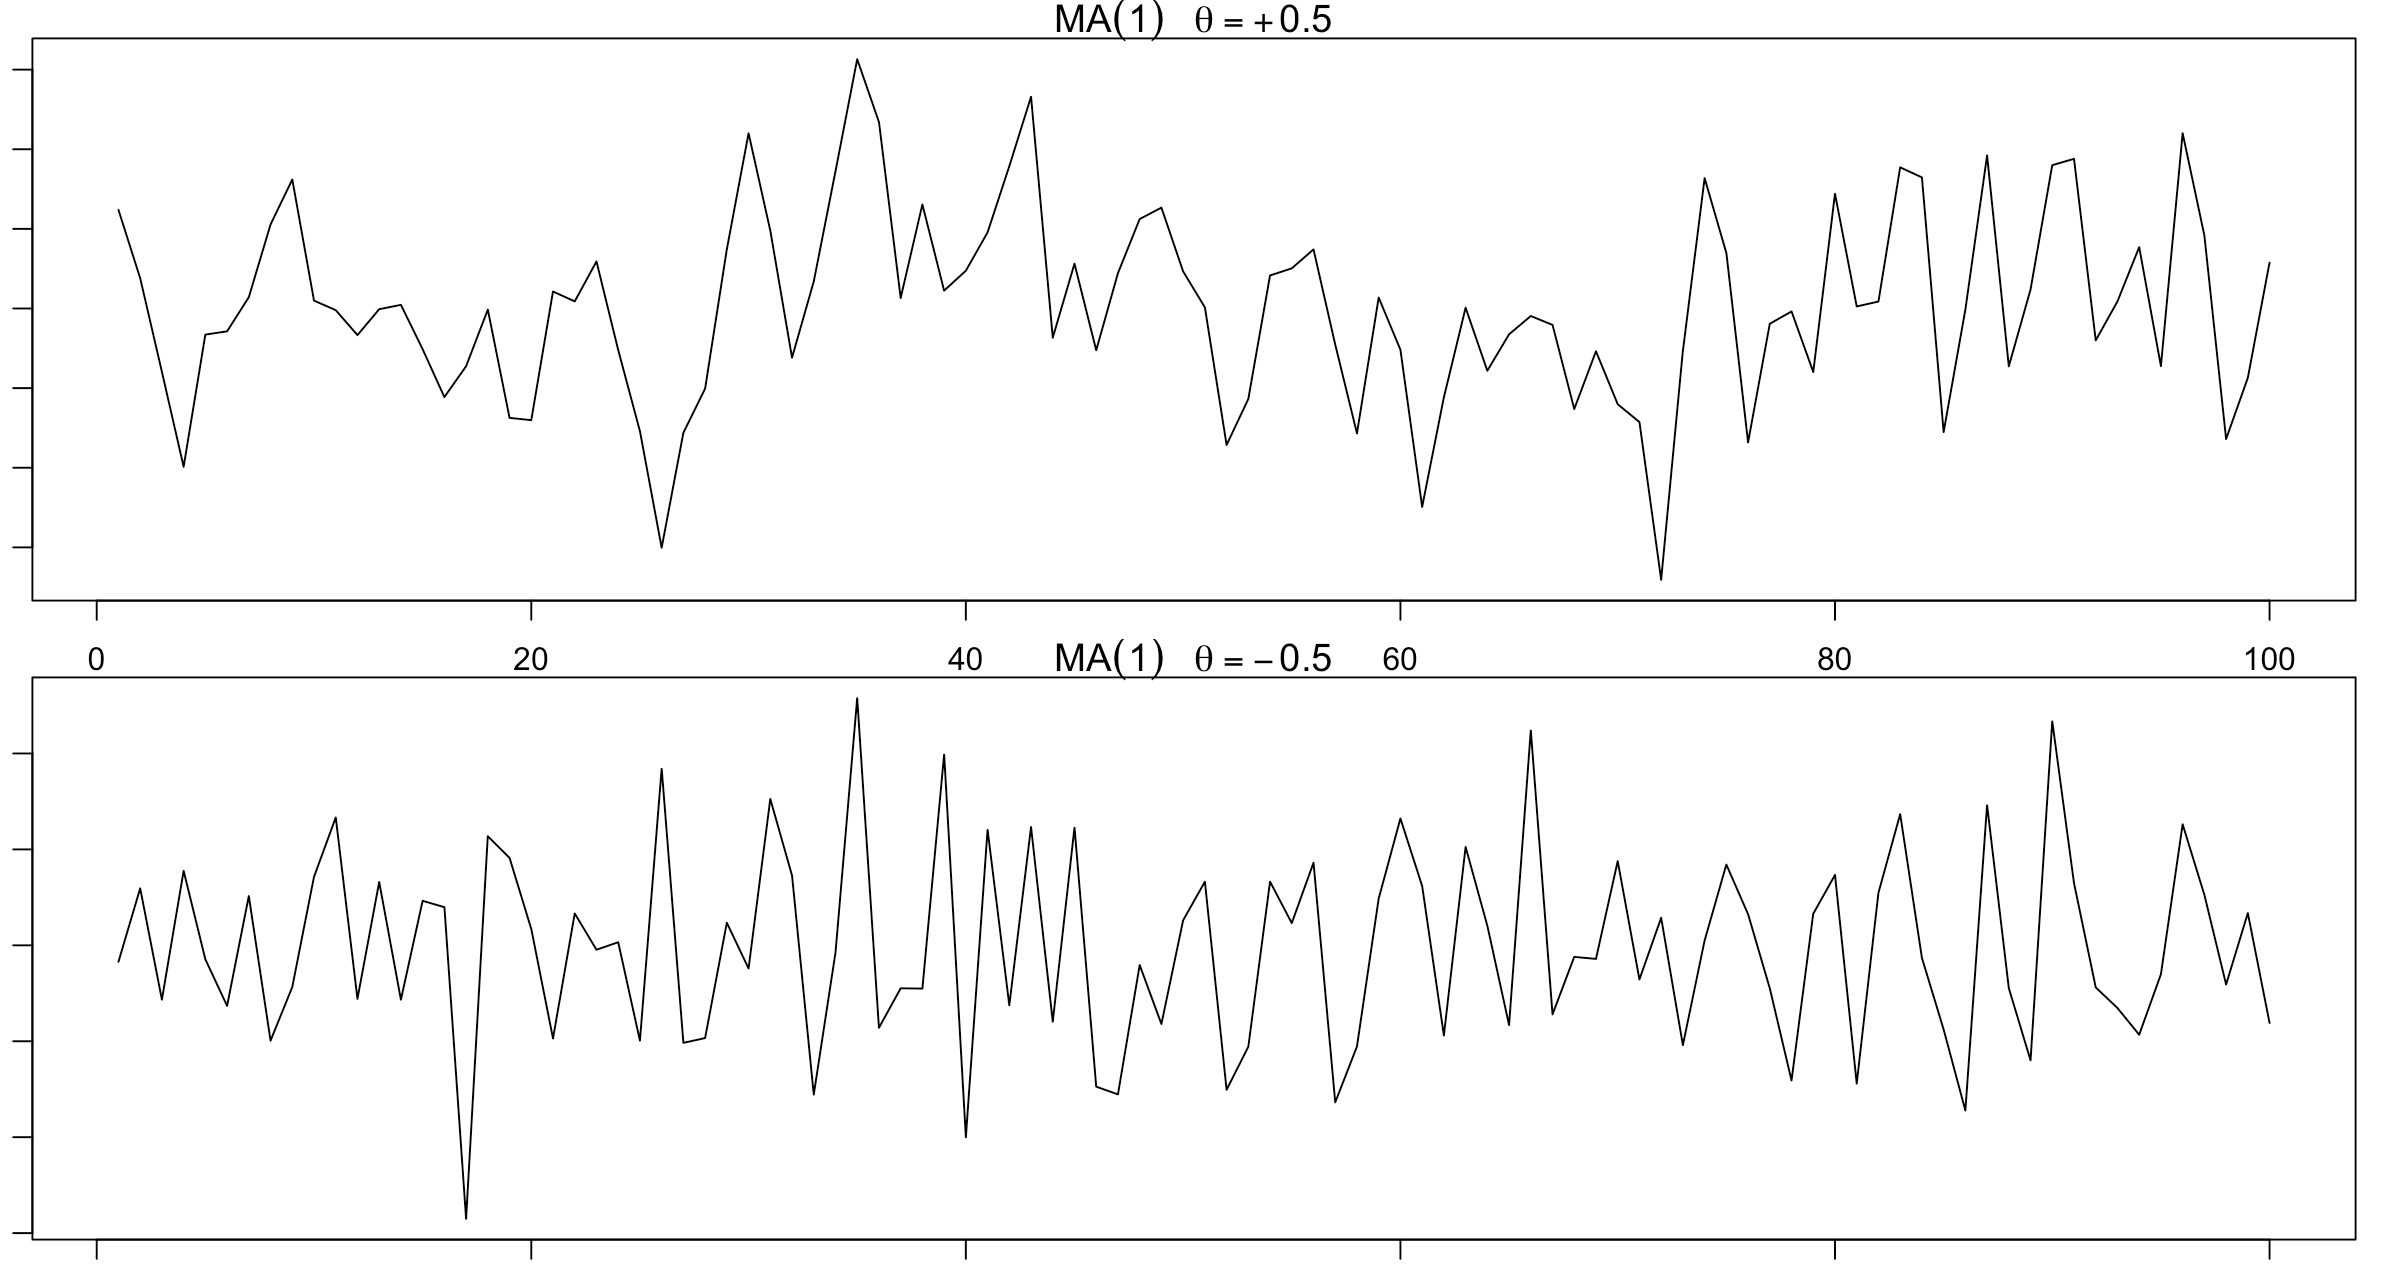
\includegraphics[width=\linewidth]{ma.png}}
	\caption{Procesos de medias móviles. Arriba: parámetro $\theta=+0.5$. Abajo: parámetro $\theta=-0.5$}\label{fig9}
\end{figure}

%\end{frame}

%---------------------------------------------------------
%---------------------Slide 38--------------------------
%\begin{frame}
%\frametitle{Identificaci\'on modelo MA }
\pagebreak
\subsubsection{Identificaci\'on modelo MA }
Para la identificaci\'on de todos los componentes del modelo MA, tal como vimos para el modelo AR, se utiliza la funci\'on de autocorrelaci\'on (AFC) y la funci\'on de autocorrelaci\'on parcial (PAFC), y as\'{\i} se procede a la identificaci\'on de los componentes, en base a los gr\'aficos de los distintos modelos te\'oricos.

\begin{figure}[H]
	\centering
	\textbf{Autocorrelograma de proceso de media móvil MA(1), $\theta=+0.5$}\par\medskip
	\fcolorbox{green}{blue}{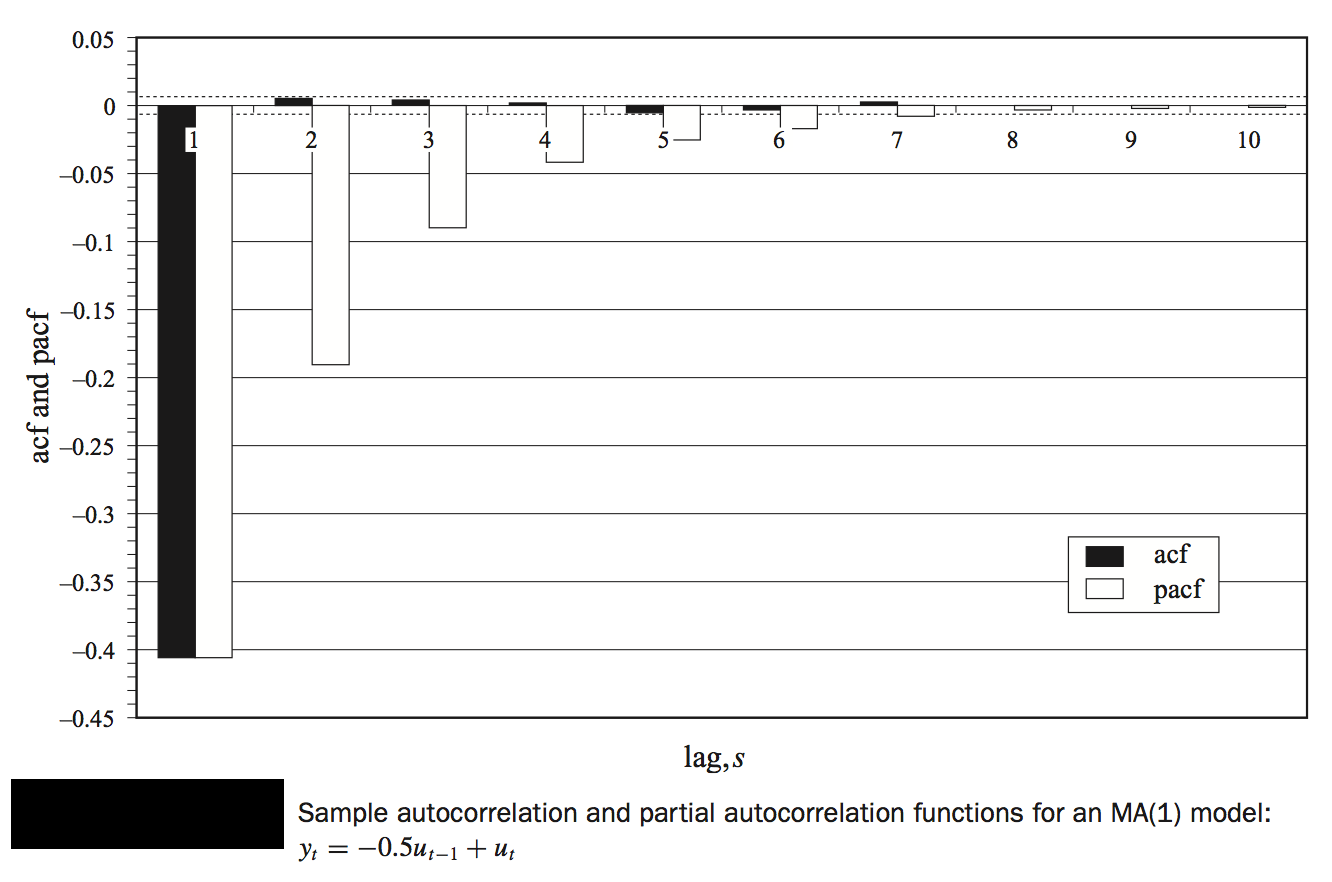
\includegraphics[scale=0.3]{idMA1.png}}
	\caption{Autocorrelogramas para diferentes retardos de proceso de media móvil con $\theta=+0.5$(lags). ACF(barras negras), PACF(barras blancas).}\label{fig10}
\end{figure}


%\end{frame}
%---------------------------------------------------------
%---------------------Slide 39--------------------------
%\begin{frame}
%\frametitle{Identificaci\'on modelo ARMA }
\subsection{Identificaci\'on modelo ARMA}


\begin{figure}[H]
	\centering
	\textbf{Autocorrelograma de proceso de media móvil MA(1), $\theta=-0.5$ }\par\medskip
	\fcolorbox{green}{blue}{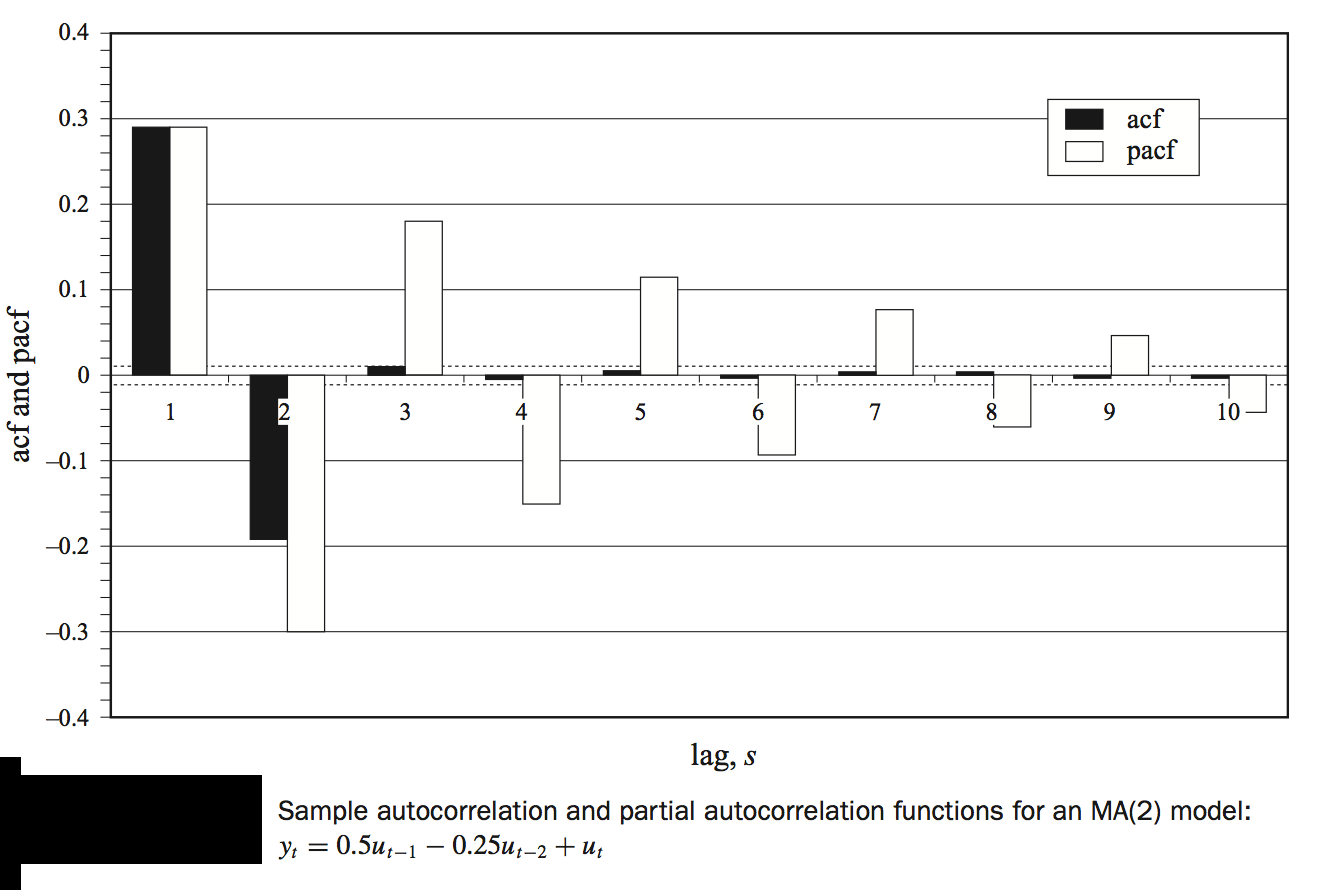
\includegraphics[width=\linewidth]{idMA2.png}}
	\caption{Autocorrelogramas para diferentes retardos de proceso de media móvil con $\theta=-0.5$(lags). ACF(barras negras), PACF(barras blancas).}\label{fig13}
\end{figure}


%\end{frame}
%---------------------------------------------------------
%---------------------Slide 40--------------------------
%\begin{frame}
%\frametitle{Modelos ARIMA: modelando el corto plazo}

%\only<1|handout:1>{
%\begin{block}{Definici\'on: Modelo ARMA - $ARMA (r,q)$}
%
%Una serie de tiempo $\{x_t, t = 0, \pm1, \pm2 , \dots{} \}$ es un proceso ARMA(p, q), si es estacionario y	
%\begin{equation}
%x_t =  \phi_1 x_{t-1} +  \phi_2 x_{t-2} + \dots{} +  \phi_p x_{t-p} + \epsilon_t + \theta_1 \epsilon_{t-1} +  \theta_2 \epsilon_{t-2} + \dots{} +  \theta_q \epsilon_{t-q} 
%\end{equation}
%
%Los par\'ametros p y q se llaman \'ordenes autoregresivas y promedios m\'oviles, respectivamente. \\
%\vspace{4mm}	
%Si $x_t$ tiene una media distinta de cero $\mu$, establecemos que $\alpha = \mu (1-\theta_1, \dots{} -\theta_q)$ y podemos re-escribimos el modelo como:
%
%\begin{equation}
%x_t = \alpha + \phi_1 x_{t-1} + \dots{} + \phi_p x_{t-p} + w_t +\theta_1  \epsilon_{t-1} + \dots{} + \theta_q  \epsilon_{t-q} .
%\end{equation}
%
%\end{block}
%}
\pagebreak
\begin{mdframed}[style=MyFrame]
	\begin{definition}\label{def7}
		\textbf{Definici\'on:  $Modelo ARMA - ARMA (r,q)$:}\\
Una serie de tiempo $\{x_t, t = 0, \pm1, \pm2 , \dots{} \}$ es un proceso ARMA(p, q), si es estacionario y	
\begin{equation}
x_t =  \phi_1 x_{t-1} +  \phi_2 x_{t-2} + \dots{} +  \phi_p x_{t-p} + \epsilon_t + \theta_1 \epsilon_{t-1} +  \theta_2 \epsilon_{t-2} + \dots{} +  \theta_q \epsilon_{t-q} 
\end{equation}

Los par\'ametros p y q se llaman \'ordenes autoregresivas y promedios m\'oviles, respectivamente. \\
\vspace{4mm}	
Si $x_t$ tiene una media distinta de cero $\mu$, establecemos que $\alpha = \mu (1-\theta_1, \dots{} -\theta_q)$ y podemos re-escribimos el modelo como:

\begin{equation}
x_t = \alpha + \phi_1 x_{t-1} + \dots{} + \phi_p x_{t-p} + w_t +\theta_1  \epsilon_{t-1} + \dots{} + \theta_q  \epsilon_{t-q} .
\end{equation}		
	\end{definition}
\end{mdframed}
%\end{frame}
%---------------------------------------------------------
%---------------------Slide 41 --------------------------
%\begin{frame}
%\frametitle{Modelos ARIMA: modelando el corto plazo}

%\textbf{Invertibilidad}
\subsection{Invertibilidad}
Una serie temporal es invertible si los errores se pueden invertir en una representaci\'on de observaciones pasadas. As\'{\i} por ejemplo, como ya vimos, el modelo AR es siempre invertible.
En el caso del modelo ARMA, las ra\'{\i}ces de las siguientes ecuaciones deben ser analizadas para garantizar invertibilidad.

\begin{equation}
\phi (z) = 1 + \phi_1 z + \phi_2 z^2 + \dots{} + \phi_p z^p
\end{equation}

\begin{equation}
\theta(z) =  1 + \theta_1 z + \theta_2 z^2 + \dots{} + \theta_q z^q
\end{equation}

En particular el modelo ARMA ser\'a invertible si y solo si $\theta(z) \ne 0$ para $|z| \le 1$
En general, los valores propios son la soluci\'on del $det (A - \lambda I)$ = 0, vemos que este es casi el polinomio caracter\'{\i}stico de las ecuaciones que definimos arriba. Por lo tanto, vemos que los valores propios de A son el inverso de las ra\'{\i}ces del polinomio caracter\'{\i}stico, y esa convergencia de la iteraci\'on hacia atr\'as ocurre cuando las ra\'{\i}ces del polinomio caracter\'{\i}stico se encuentran fuera del c\'{\i}rculo unitario.

%\end{frame}
%---------------------------------------------------------
%---------------------Slide 42 --------------------------
%\begin{frame}
%\frametitle{Modelos ARIMA: modelando el corto plazo}

%\textbf{Estacionaridad e Invertibilidad}
\subsection{Estacionaridad e Invertibilidad}
Wold demostr\'o que todos los procesos estoc\'asticos estacionarios de covarianza podr\'{\i}an descomponerse como la suma de
procesos determin\'{\i}sticos y linealmente indeterministas los cuales no estaban correlacionados con todos los rezagos; es decir,
si $y_t$ es la covarianza estacionaria, entonces:

\begin{equation}
y_t = x_t + z_t
\end{equation}

donde $x_t$ es un proceso determinista estacionario en covarianza y $z_t$ es linealmente indeterminista,
con $Cov (x_t, z_s) = 0$ para todas los $t$ y $s$. Este resultado proporciona una base te\'orica para la propuesta de Box y Jenkins  para modelar procesos estacionarios de covarianza escalar (desestacionalizados) como son los procesos ARMA.
%\end{frame}
%---------------------------------------------------------
%---------------------Slide 43--------------------------
%\begin{frame}
%\frametitle{Modelos ARIMA: modelando el corto plazo}

%\textbf{Modelos ARMA (p,q)}
\subsection{Modelos ARMA (p,q)}

Como se indic\'o anteriormente, cuando $q$ = 0, el modelo se denomina modelo autoregresivo de orden $p$, $AR (p)$, y cuando $p$ = 0, el modelo se denomina modelo de promedio m\'ovil de orden $q$, $MA (q)$. \\
Es \'util escribir los modelos ARIMA usando el operador AR y el operador MA descritos anteriormente. En particular, el modelo $ARMA (p, q) $ puede escribirse entonces en forma concisa como:

\begin{equation}
\phi (B) x_t = \theta (B) \epsilon_t.
\end{equation}
%\textbf{Modelos ARIMA (p, i, q)}
\subsection{Modelos ARIMA (p, i, q)}
El modelo ARMA gana su I y se convierte en ARIMA cuando debe ser integrado para lograr estacionaridad. El \'{\i}ndice $I$ ser\'a entonces el numero de veces que debe ser diferenciado.
%\end{frame}

%---------------------------------------------------------
%---------------------Slide 44--------------------------
%\begin{frame}
%\frametitle{Identificaci\'on modelo ARMA }
\subsection{Identificaci\'on modelo ARMA}

Para la identificaci\'on de todos los componentes del modelo ARMA se utiliza la funci\'on de autocorrelaci\'on (AFC) y la funci\'on de autocorrelaci\'on parcial (PAFC), y as\'{\i} se procede a la identificaci\'on de los componentes estacional y no estacional por separado, en base a los gr\'aficos de los distintos modelos te\'oricos.

\begin{figure}[H]
	\centering
	\textbf{Proceso autoregresivo de media móvil de orden (1,1): ARMA(1,1)}\par\medskip
	\fcolorbox{green}{blue}{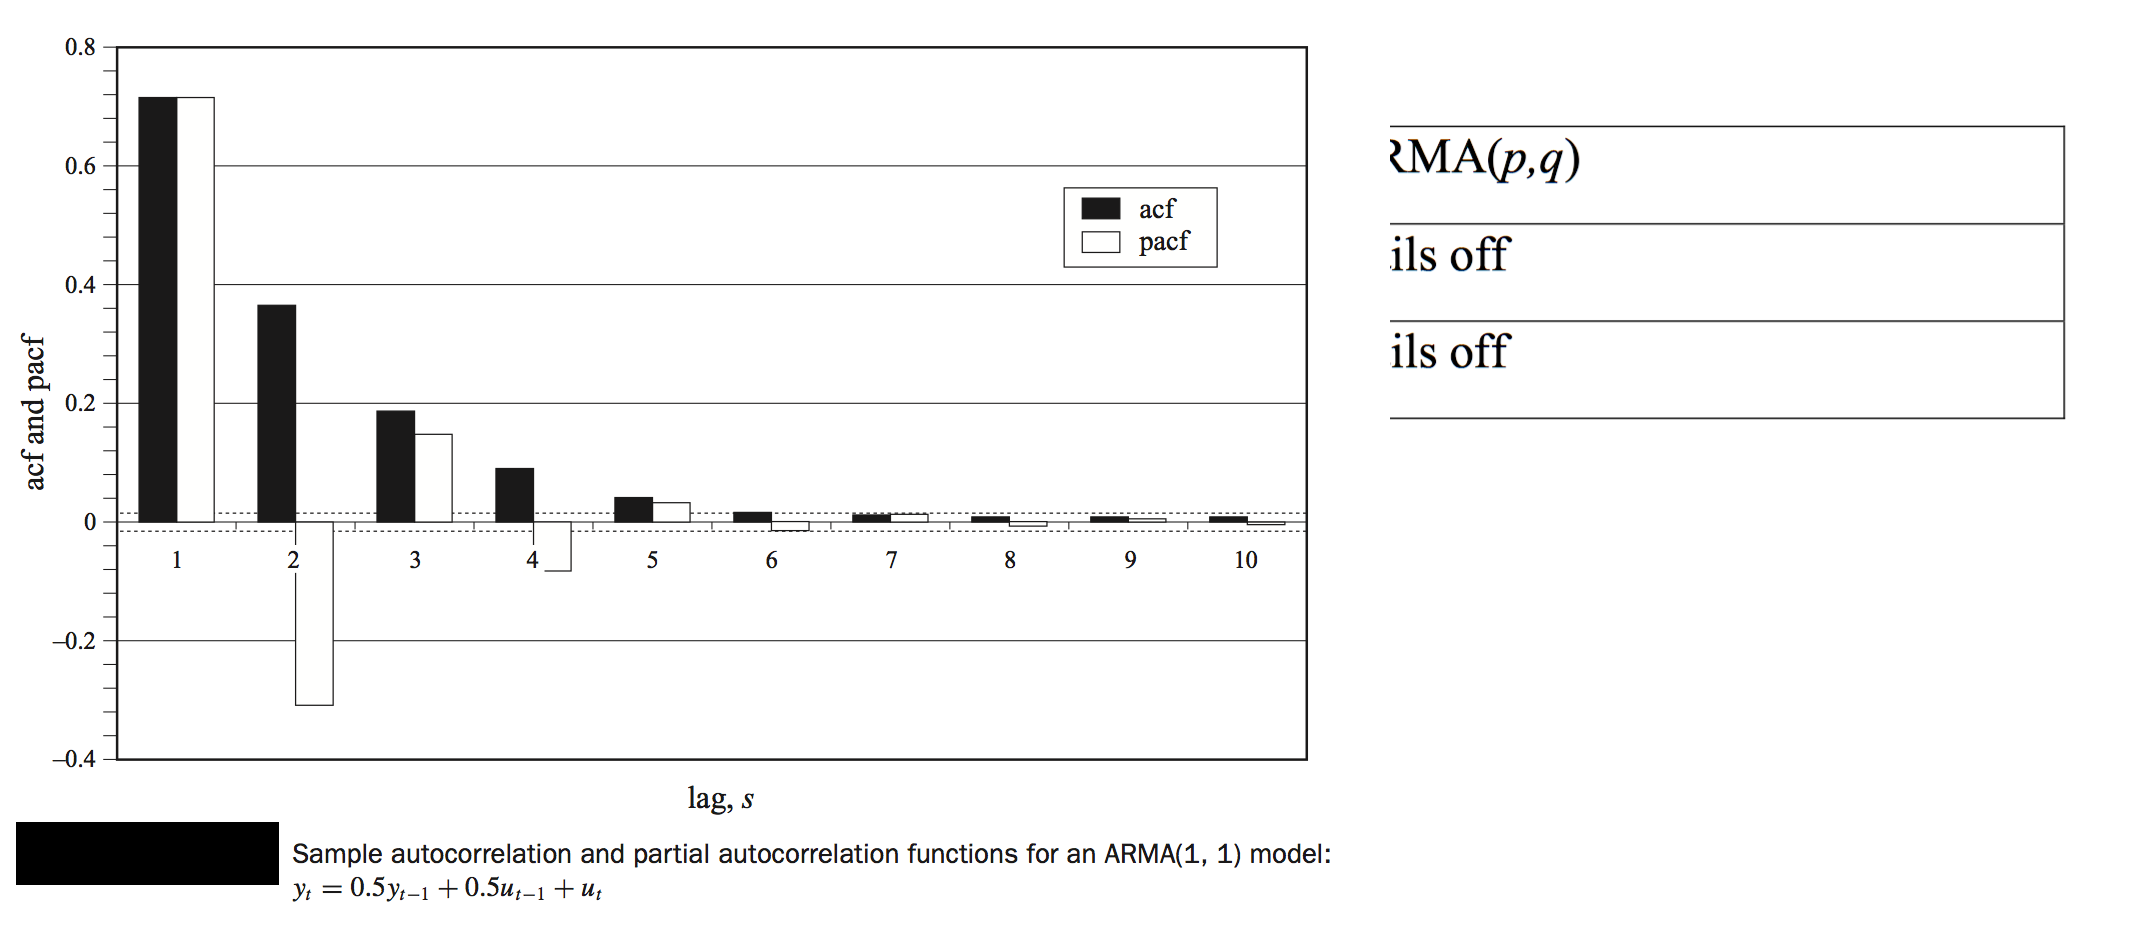
\includegraphics[width=\linewidth]{idARMA.png}}
	\caption{Autocorrelogramas para diferentes retardos(lags) para un proceso ARMA(1,1)}\label{fig16}
\end{figure}

%\end{frame}
%---------------------------------------------------------
%---------------------Slide 45--------------------------
%\begin{frame}
%\frametitle{Identificaci\'on modelo ARMA }

En resumen tendremos:

\begin{figure}[H]
	\centering
	\textbf{En resumen tendremos:}\par\medskip
	\fcolorbox{green}{blue}{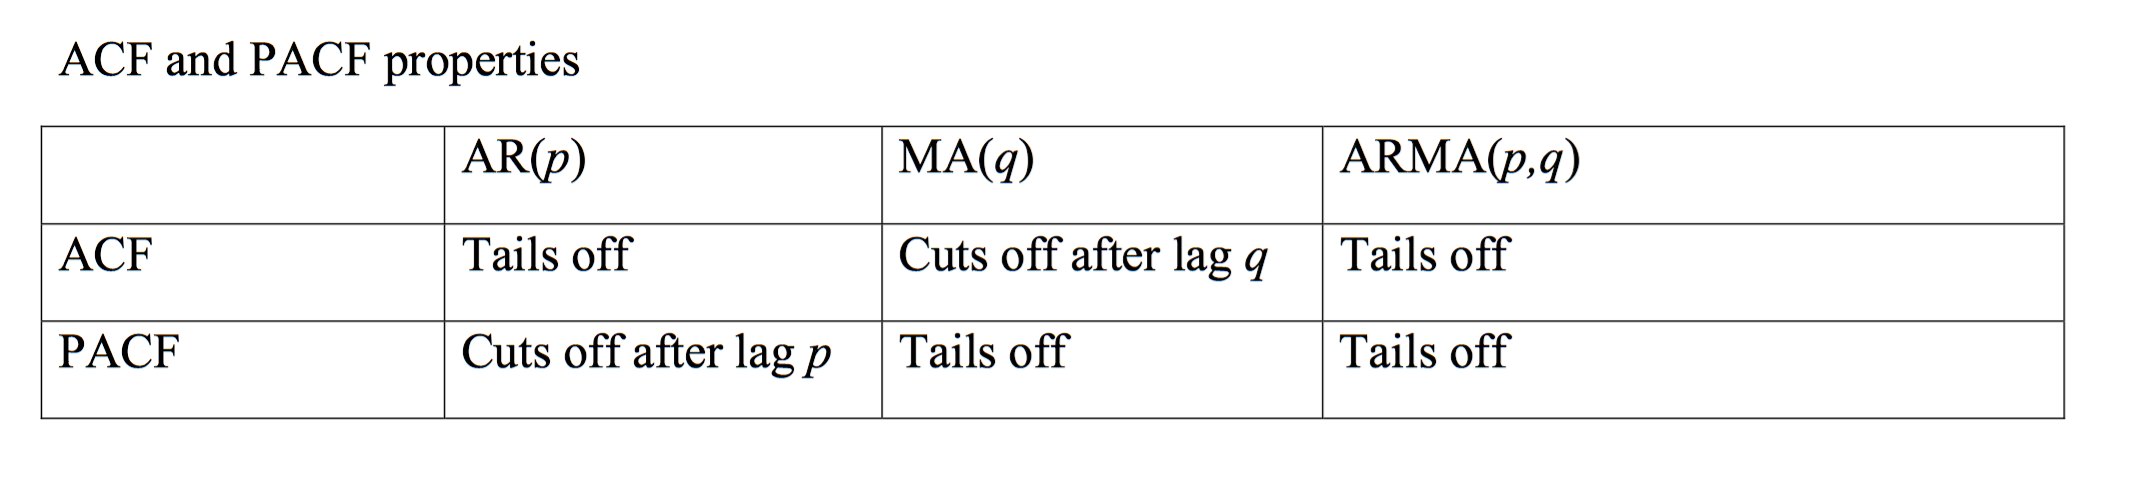
\includegraphics[width=\linewidth]{resumenARMA.png}}
	\caption{Tabla resumen de los modelos AR(p),MA(q) y ARMA(p,q), con sus respectivos resultados esperados para las funciones de autocorrelación(ACF) y autocorrelación parcial(PACF)}\label{fig14}
\end{figure}

%\end{frame}
%---------------------------------------------------------
%---------------------Slide 46--------------------------
%\begin{frame}
%\frametitle{Modelos SARIMA (p,q)}
\subsection{Modelos SARIMA (p,q)}

Los modelos ARIMA tambi\'en son capaces de modelar una amplia gama de datos estacionales. Los llamados  modelos SARIMA, Seasonal ARIMA models, se obtienen al incluir t\'erminos estacionales adicionales en los modelos ARIMA que hemos visto hasta ahora, de la siguiente manera:

\begin{equation}
ARIMA (p,d,q)(P,D,Q)m
\end{equation}

donde m = n\'umero de per\'{\i}odos por temporada. \\
Usamos la notaci\'on en may\'usculas para las partes estacionales del modelo y la notaci\'on en min\'usculas para las partes no estacionales del modelo.\\
La parte estacional del modelo consiste en t\'erminos que son muy similares a los componentes no estacionales del modelo, pero implican retrocesos del per\'{\i}odo estacional. \\

%\end{frame}
%\end{section}
%---------------------------------------------------------
%---------------------Slide 47--------------------------
%\begin{section}{Evaluaci\'on estad\'{\i}stica de un Modelo ARIMA}
%\begin{frame}
%\frametitle{Evaluaci\'on estad\'{\i}stica de un Modelo ARIMA}
\subsubsection[evaluación]{Evaluaci\'on estad\'{\i}stica de un Modelo ARIMA}
Se debe evaluar:
%\only<1->{
\begin{itemize}
\item[A] \textbf{Significancia estad\'{\i}stica de los par\'ametros} 
Los coeficientes obtenidos en la estimaci\'on que no sean significativamente distintos de cero, a un nivel de significancia del $5\%$, no son necesarios, por lo que deben eliminarse.
\item[B] \textbf{Estacionariedad e invertibilidad del modelo estimado.} Para valores de los coeficientes estimados pr\'oximos a la frontera de la no-estacionariedad, es conveniente llevar a cabo un test de ra\'{\i}ces unitarias.
\item[C] \textbf{Estabilidad del modelo estimado.} Aunque los par\'ametros sean significativos, el modelo puede ser rechazado si existe una fuerte correlaci\'on entre los par\'ametros del modelo. Esto ocurre cuando el coeficiente de correlaci\'on tiene un valor absoluto superior a 0,7, entonces es conveniente probar con modelos alternativos.
\end{itemize}
%} 

%\end{frame}

%---------------------------------------------------------
%---------------------Slide 48--------------------------
%\begin{frame}
%\frametitle{Sobre la Selecci\'on de Modelos}
\subsection{Sobre la Selecci\'on de Modelos}

Puede ocurrir que varios modelos describan satisfactoriamente la serie temporal, por lo que sea necesario seleccionar el modelo m\'as adecuado. Este proceso de selecci\'on puede ser sencillo o un poco m\'as complejo, por lo que es necesario recurrir a criterios de selecci\'on de modelos.\\
%\par
Los criterios m\'as comunes en la selecci\'on de modelos son el AIC (Akaike Information Criterion) y el BIC (Bayesian Information Criterion) que es una extensi\'on bayesiana del primero. 

%\end{frame}

%---------------------------------------------------------
%---------------------Slide 49 --------------------------
%\begin{frame}
%\frametitle{Criterios de Informaci\'on}
\subsubsection{Criterios de Informaci\'on}

%\only<1|handout:1>{
%\begin{block}{Definici\'on: Akaike Information Criterion}
%\begin{equation*}
%AIC = log \hat{\sigma_k^2} + \frac{n+2k}{n} 
%\end{equation*}
%\end{block}
%}
\begin{mdframed}[style=MyFrame]
	\begin{definition}\label{def8}
		\textbf{Definici\'on: Akaike Information Criterion}
		\begin{equation*}
		AIC = log \hat{\sigma_k^2} + \frac{n+2k}{n} 
		\end{equation*}
	\end{definition}
\end{mdframed}
\vspace{4mm}	
Donde $\hat{\sigma_k^2} = \frac{SSE_k}{n}$, donde $k$ es el n\'umero de par\'ametros del modelo, $n$ el tama\~no de la muestra, y $SSE_k$ equivale a la suma de los residuos al cuadrado bajo el modelo $k$ ($SSE_k=\sum_{t=1}^{n}(x_t-\bar{x})^2$).\\
%\par
%\vspace{4mm}	
El valor de $k$ que produce el m\'{\i}nimo AIC representa el mejor modelo. La idea es que minimizar $\hat{\sigma_k^2}$ representa un objetivo razonable, excepto que disminuye mon\'otonamente a medida que $k$ aumenta. Por lo tanto, debemos penalizar la varianza del error por un t\'ermino proporcional al n\'umero de par\'ametros.

%\end{frame}
%---------------------------------------------------------
%---------------------Slide 50 --------------------------
%\begin{frame}
%\frametitle{Criterios de Informaci\'on}
%
%\only<1|handout:1>{
%	\begin{block}{Definici\'on: Bias Corrected}
%		\begin{equation*}
%		AICc = log \hat{\sigma_k^2} + \frac{n+k}{n-k-2} 
%		\end{equation*}
%	\end{block}
%}
\begin{mdframed}[style=MyFrame]
	\begin{definition}\label{def15}
		\textbf{Definici\'on:  Bias Corrected}
		\begin{equation*}
				AICc = log \hat{\sigma_k^2} + \frac{n+k}{n-k-2} 
		\end{equation*}
	\end{definition}
\end{mdframed}

%\only<1|handout:1>{
%	\begin{block}{Definici\'on: Bayesian Information Criterion - BIC}
%		\begin{equation*}
%		AICc = log \hat{\sigma_k^2} + \frac{k log n}{n} 
%		\end{equation*}
%	\end{block}
%}
\begin{mdframed}[style=MyFrame]
	\begin{definition}\label{def16}
		\textbf{Definici\'on:  Bayesian Information Criterion - BIC}
		\begin{equation*}
		AICc = log \hat{\sigma_k^2} + \frac{k log n}{n} 
		\end{equation*}		
	\end{definition}
\end{mdframed}
BIC tambi\'en se conoce como el \textbf{Schwarz Information Criterion (SIC)}. Varios estudios de simulaci\'on han verificado que BIC es adecuado para obtener el orden correcto en muestras grandes, mientras que AICc tiende a ser superior en muestras m\'as peque\~nas donde el n\'umero relativo de par\'ametros es grande.

%\end{frame}

%---------------------------------------------------------
%---------------------Slide 51--------------------------
%\begin{frame}
%\frametitle{Sobre la Selecci\'on de Modelos}

\pagebreak En \'ultimo t\'ermino un modelo es mejor que otro si su predicci\'on es mejor. Por otro lado, diremos que \textbf{una predicci\'on, es mejor que otra, cuando comete un menor error extra-muestral.}\\
%\par
As\'{\i}, la precisi\'on de los m\'etodos utilizados para pronosticar se pueden medir por ejemplo a trav\'es de la funci\'on de p\'erdida: \textbf{Error cuadr\'atico medio - Mean Square Error (MSE)}, con el fin de comprender qu\'e modelo proporciona un mejor pron\'ostico extra-muestral sobre otro. Esto es:

\begin{equation}
\textbf{MSE}=\frac{1}{T} \sum_{t=1}^T (x_t-\hat{x}_t)^2
\label{MSE}
\end{equation}

donde $x_t$ corresponde al valor real de la serie en el tiempo $t$ y $\hat{x}_{t}$ corresponde al valor pronosticado por el modelo propuesto en el mismo instante.

%\end{frame}

%---------------------------------------------------------
%---------------------Slide 52--------------------------
%\begin{frame}
%\frametitle{Sobre la Selecci\'on de Modelos}

Otros criterios de selecci\'on de modelos que consideran el error extra-muestral son: 
\begin{itemize}
	\item i) el \textbf{Error Absoluto Medio (EAM) - mean absolute deviation (MAD)},
	\begin{equation}
	\textbf{MAD}=\frac{1}{T} \sum_{t=1}^T |x_t-\hat{x}_t|
	\label{MAD}
	\end{equation} y 
	\item ii) \textbf{Error Absoluto Porcentual Medio (EAPM) - mean absolute percentage error (MAPE)}
	\begin{equation}
	\textbf{MAPE}=\frac{1}{T} \sum_{t=1}^T \left| 1 - \frac{x_t}{\hat{x}_t}\right|
	\label{MAPE}
	\end{equation}
	 
\end{itemize}

%\begin{equation}
%\textbf{MAD}=\frac{1}{T} \sum_{t=1}^T |x_t-\hat{x}_t|
%\label{MAD}
%\end{equation}

%\begin{equation}
%\textbf{MAPE}=\frac{1}{T} \sum_{t=1}^T \left| 1 - \frac{x_t}{\hat{x}_t}\right|
%\label{MAPE}
%\end{equation}
%\end{frame}

%---------------------------------------------------------
%---------------------Slide 53 --------------------------
%\begin{frame}
%\frametitle{Ejemplo IPC en Chile}
\subsection{Ejemplo IPC en Chile}
Considerando data mensual del IPC desde enero del 2013 a la fecha en Chile, obtenida de la p\'agina del Banco Central, intetnaremos predecir el IPC (serie original).
%\only<1|handout:1>{
%\begin{exampleblock}{C\'odigo en R}
%rm(list=ls())\\
%data$<-$read.csv (``ipc.csv")\\
%ipc $<-$ ts(data[,2],start = c(2013,1), end=c(2018, 6), frequency = 12)\\
%plot.ts(ipc, xlab='Years', ylab = ``Indice de Precios al Comsumidor')\\
%
%\end{exampleblock}
%}
\lstset{caption=Ejemplo IPC en Chile ,framexleftmargin=5mm, frame=shadowbox, rulesepcolor=\color{green}}
\begin{lstlisting}[title={‘Código R: Ejemplo IPC en Chile’},basicstyle=\ttfamily]{}
rm(list=ls())
data<-read.csv ("ipc.csv")
ipc <- ts(data[,2],start = c(2013,1), end=c(2018, 6),
		frequency = 12)
plot.ts(ipc,xlab='Years',ylab='Indice de Precios al Comsumidor')
\end{lstlisting}
%\end{frame}
%---------------------------------------------------------
%---------------------Slide 54--------------------------
%\begin{frame}
%\frametitle{Ejemplo IPC en Chile}

\begin{figure}[H]
	\centering
	\textbf{Ejemplo IPC en Chile.}\par\medskip
	\fcolorbox{green}{blue}{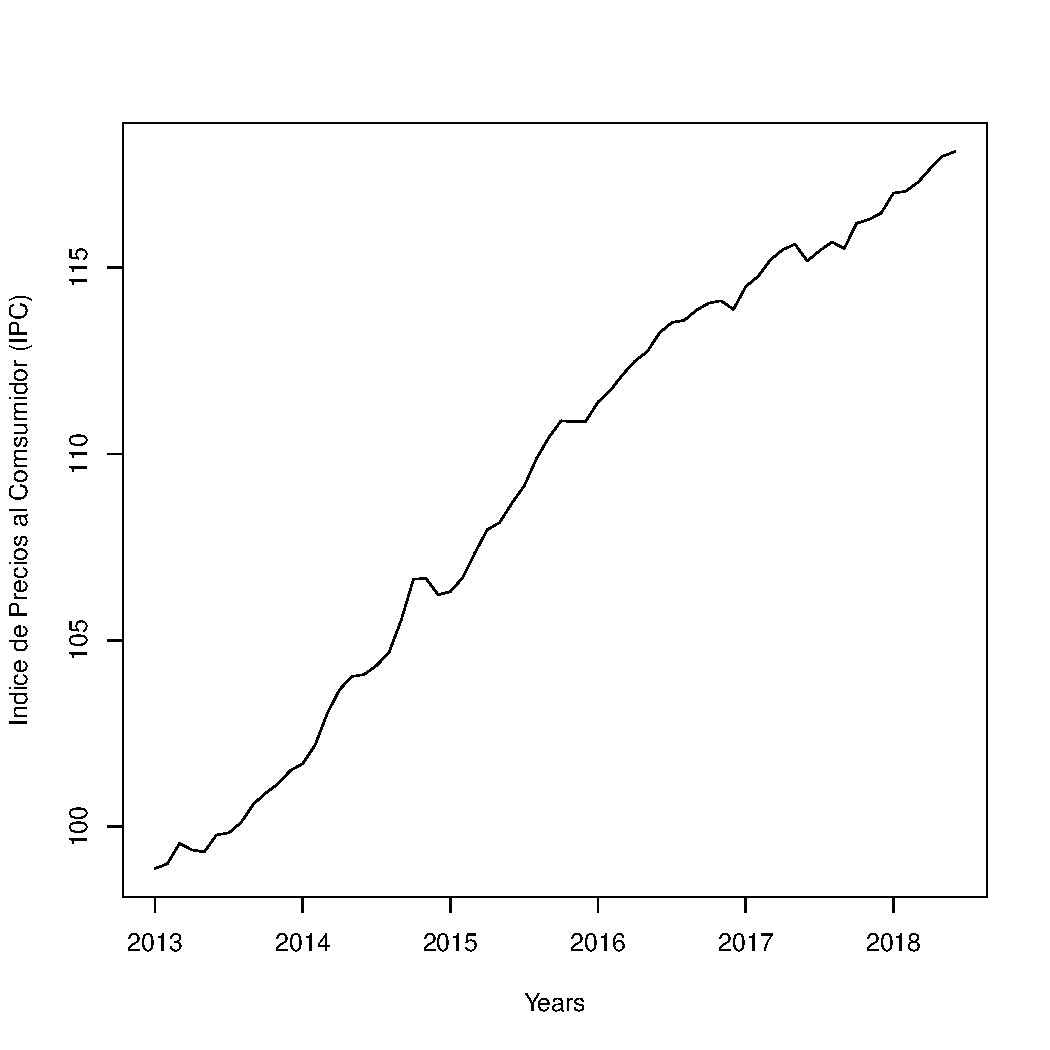
\includegraphics[width=\linewidth]{ipc.pdf}}
	\caption{Serie de tiempo del índice de precios al consumidor (IPC) en Chile.}\label{fig18}
\end{figure}

%\end{frame}

%---------------------------------------------------------
%---------------------Slide 55 --------------------------
%\begin{frame}
%\frametitle{Ejemplo IPC en Chile}
\pagebreak
\subsubsection{Encontrando el orden del modelo. Tendencia, estacionaridad, autocorrelaci\'on.}
%\only<1|handout:1>{
%\begin{exampleblock}{C\'odigo en R}
%
%$\#$ Descomposici\'on\\
%fit $<-$ stl(ipc, s.window=``period")\\
%plot(fit)\\
%
%$\#$ Test de ra\'{\i}z unitaria\\
%adf.test(ipc)\\
%adf.test(diff(ipc))\\
%
%$\#$ Funci\'on de autocorrelaci\'on (AFC) y autocorrelaci\'on parcial (PAFC)\\
%acf(diff(ipc),lag=36,lwd=3)\\
%pacf(diff(ipc),lag=36,lwd=3)\\
%\end{exampleblock}
%}
\lstset{caption=Ejemplo ,framexleftmargin=5mm, frame=shadowbox, rulesepcolor=\color{green}}
\begin{lstlisting}[title={‘Código R: Tendencia, estacionaridad, autocorrelación. ’},basicstyle=\ttfamily]{}
#Descomposicion
fit <- stl(ipc, s.window="period")
plot(fit)
library("tseries")
#TestRaizUnitaria
adf.test(ipc)
adf.test(diff(ipc))
#FuncionAutocorrelacion_yAutocorrelacionParcial
acf(diff(ipc),lag=36,lwd=3)
pacf(diff(ipc),lag=36,lwd=3)
\end{lstlisting}

%\end{frame}
%---------------------------------------------------------
%---------------------Slide 56--------------------------
%\begin{frame}
%\frametitle{Ejemplo IPC en Chile}

%\textbf{Descomposici\'on\ de la serie}\\
\subsection{Descomposici\'on\ de la serie}

\begin{figure}[H]
	\centering
	\textbf{Ejemplo IPC: Descomposición de la serie de IPC}\par\medskip
	\fcolorbox{green}{blue}{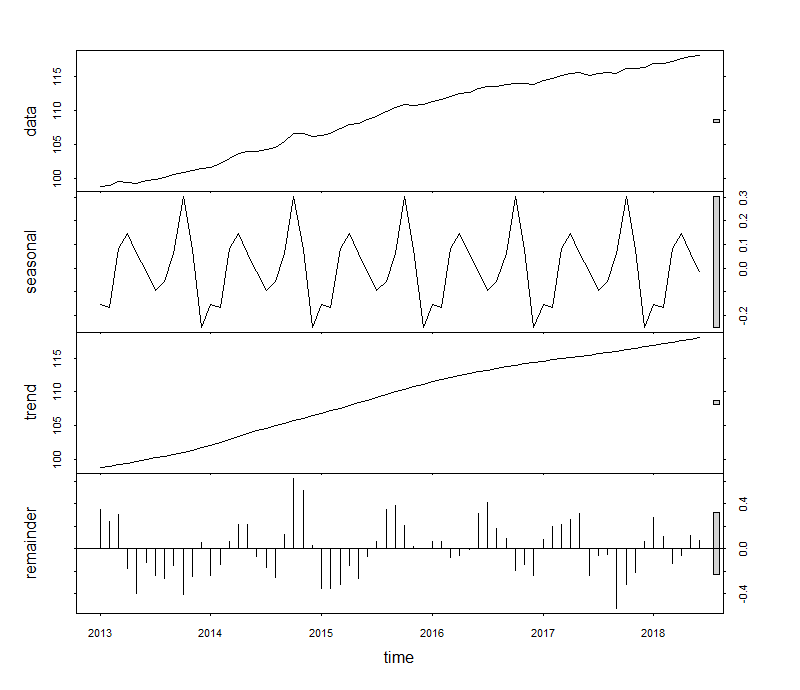
\includegraphics[width=\linewidth]{ipcdecomp.png}}
	\caption{Diferentes componentes de la serie: data: serie original de IPC; seasonal: componente estacional; trend: tendencia de la serie; remainder: componentes irregulares.}\label{fig20}
\end{figure}

%\end{frame}

%---------------------------------------------------------
%---------------------Slide 57--------------------------
%\begin{frame}
%\frametitle{Ejemplo IPC en Chile}

%\textbf{Test de ra\'{\i}z unitaria}\\
%\vspace{4mm}	
%Augmented Dickey-Fuller Test\\
%data:  ipc\\
%Dickey-Fuller = -0.11148, Lag order = 4, p-value =0.99\\
%alternative hypothesis: stationary\\
%\vspace{4mm}	
%Augmented Dickey-Fuller Test\\
%data:  diff(ipc)\\
%Dickey-Fuller = -5.8024, Lag order = 3, p-value = 0.01\\
%alternative hypothesis: stationary\\
\begin{figure}[H]
	\centering
	\textbf{Test de ra\'{\i}z unitaria}\par\medskip
	\fcolorbox{green}{blue}{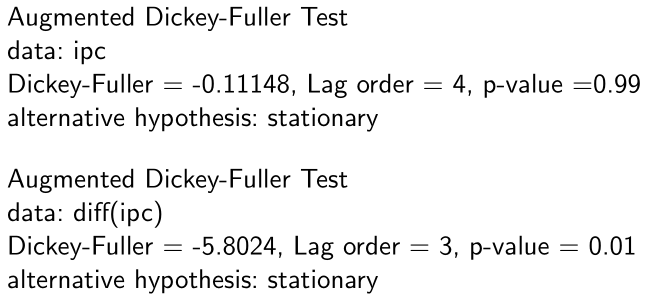
\includegraphics[width=\linewidth]{testRaizUnitIPCChile.png}}
	\caption{Test de Augmented Dickey-Füller sobre data original(ipc) y sobre primera diferencia de la data de ipc(diff(ipc))}\label{fig21}
\end{figure}
%\end{frame}

%---------------------------------------------------------
%---------------------Slide 58--------------------------
%\begin{frame}
%\frametitle{Ejemplo IPC en Chile}
%
%\textbf{Funci\'on de autocorrelaci\'on (AFC) y autocorrelaci\'on parcial (PAFC)}\\
\begin{figure}[H]
	\centering
	\textbf{Funci\'on de autocorrelaci\'on (AFC) y autocorrelaci\'on parcial (PAFC)}\par\medskip
	\fcolorbox{green}{blue}{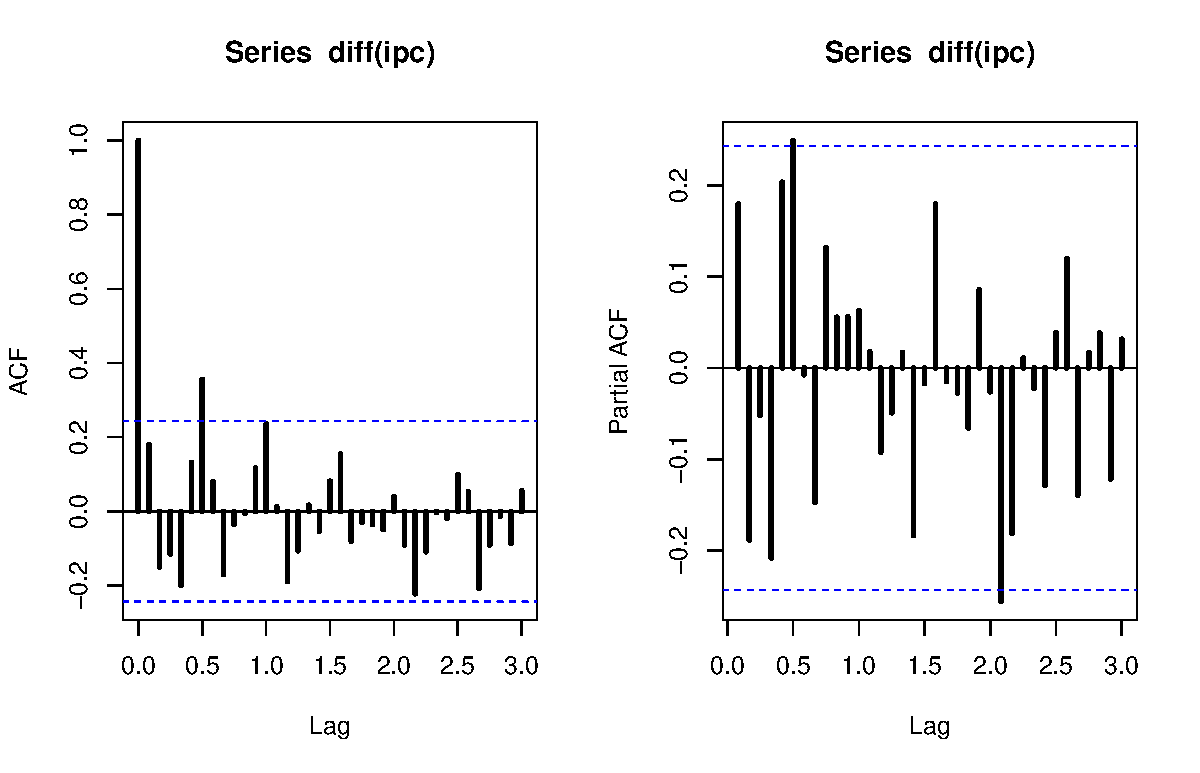
\includegraphics[width=\linewidth]{acfpacdiffipc.pdf}}
	\caption{Izquierda: autocorrelacion de serie de ipc diferenciada. Derecha: autocorrelación parcial de serie de IPC diferenciada.}\label{fig22}
\end{figure}

%\end{frame}

%---------------------------------------------------------
%---------------------Slide 59--------------------------
%\begin{frame}
%\frametitle{Ejemplo IPC en Chile}

%\textbf{Pron\'ostico.}\\
%\vspace{4mm}	
%\only<1|handout:1>{
%\begin{exampleblock}{C\'odigo en R}
%
%train.series =ipc $\left [ 1:44 \right ]$\\
%test.series = ipc $\left [ 45:62 \right ]$\\
%arima.model=arima(train.series, order=c(0,1,1))\\
%forecast=predict(arima.model, length(test.series)\\
%
%mse $<-$sum((forecast$\$$pred-test.series)$\wedge2$)/length(test.series)\\
%mad $<-$ sum(abs(forecast$\$$pred-test.series))/length(test.series)\\
%mape $<-$ sum(abs( 1 - forecast$\$$pred/test.series))/length(test.series)\\
%
%fit $<-$ auto.arima(ipc)\\
%summary(fit)\\
%plot(fit)\\
%mape $<-$ sum(abs(1 - test.series/f$[[``mean"]])$)/length(test.series)\\
%accuracy(fit)\\
%\end{exampleblock}
%}
\lstset{caption=Ejemplo ,framexleftmargin=5mm, frame=shadowbox, rulesepcolor=\color{green}}
\begin{lstlisting}[title={‘Código R: REVISAR: Diapo 59(125)’},basicstyle=\ttfamily]{}
train_series=ipc[1:44]
test_series=ipc[45:62]
arimaModel=arima(train_series, order=c(0,1,1))
forecast=predict(arimaModel, length(test_series))
mse <- sum((forecast$pred-test_series)^2)/length(test_series)
mad <- sum(abs(forecast$pred-test_series))/length(test_series)
mape <- sum(abs(1-test_series/forecast$pred))/length(test_series)
fit <- auto.arima(ipc)
summary(fit)
plot(fit)

mape <- 100*sum(abs(1-test_series/f[["mean"]]))/length(test_series)
accuracy(fit)
\end{lstlisting}

%\end{frame}

%---------------------------------------------------------
%---------------------Slide 60--------------------------
%\begin{frame}
%\frametitle{Ejemplo IPC en Chile}
%\textbf{output ARIMA (0, 1, 1) }\\
%\vspace{4mm}	
%Call:\\
%arima(x = train.series, order = c(0, 1, 1))\\
%
%Coefficients:\\
%\hspace{3em}ma1\\
%\hspace{2.5em}$0.8205$\\
%s.e.\hspace{1em}$ 0.0906$\\
%
%$\sigma^2$ estimated as $0.1029:  log likelihood = -12.68,  aic = 29.37$\\
%\vspace{4mm}
%\textbf{forecast ARIMA (0, 1, 1) }\\
%mse
%[1] 69.80031
%\end{frame}
\begin{figure}[H]
	\centering
	\textbf{Resultado-Parámetros ajuste de modelo ARIMA(0,1,1) y Error de Forecast(MSE)}\par\medskip
	\fcolorbox{green}{blue}{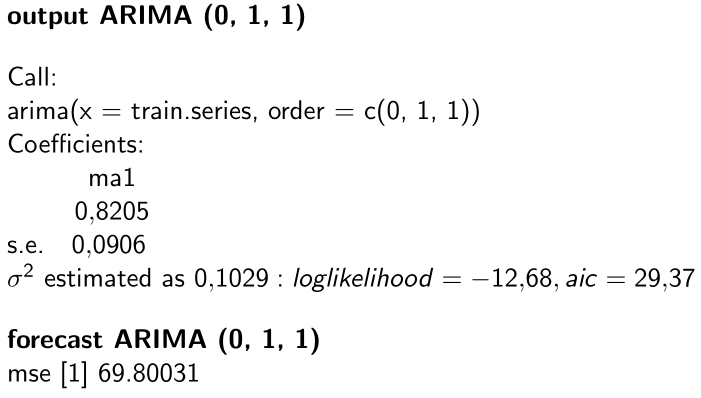
\includegraphics[width=\linewidth]{resultadoArimaD60.png}}
	\caption{Resultados del ajuste del modelo ARIMA(0,1,1) y su error de pronóstico}\label{fig24}
\end{figure}
%---------------------------------------------------------
%---------------------Slide 61--------------------------
%\begin{frame}
%\frametitle{Ejemplo IPC en Chile}
%\textbf{Pron\'ostico - output ARIMA (0, 1, 1) }\\
%\vspace{4mm}	
%$\$$pred\\
%Time Series:\\
%Start = 45 \\
%End = 54 \\
%Frequency = 1 \\
%$\left [ 1 \right ]$ $113.6141$ $113.6253$ $113.6292$ $113.6307$ $113.6311$ $113.6313$\\
%$\left [ 7 \right ]$ $113.6314$ $113.6314$ $113.6314$ $113.6314$\\
%
%$\$$se\\
%Time Series:\\
%Start = 45 \\
%End = 54 \\
%Frequency = 1 \\
%$\left [ 1 \right ]$ $0.3128668$ $0.6841962$ $0.9882296$ $1.2406559$ $1.4565974$\\
%$\left [ 6 \right ]$ $1.6465783$ $1.8174943$ $1.9738906$ $2.1188485$ $2.2545301$\\
%
%\end{frame}
\begin{figure}[H]
	\centering
	\textbf{Pronósticos de modelo ARIMA(0,1,1)}\par\medskip
	\fcolorbox{green}{blue}{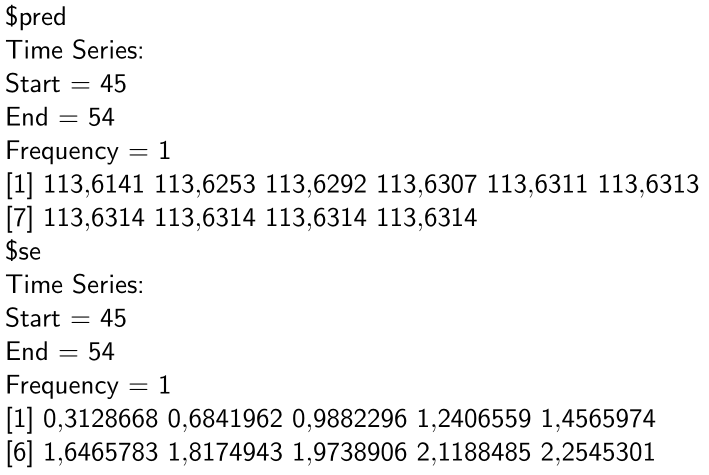
\includegraphics[width=\linewidth]{pronosticoD61.png}}
	\caption{Pronóstico ARIMA(0,1,1)}\label{fig25}
\end{figure}
%---------------------------------------------------------
%---------------------Slide 62--------------------------
%\begin{frame}
%\frametitle{Ejemplo IPC en Chile}
%\textbf{output auto.arima}\\
%
%Series: ipc \\
%ARIMA(0,1,1)(0,0,1)[12] with drift \\
%\vspace{2mm}	
%Coefficients:\\
%\hspace{5em}ma1\hspace{3em}sma1\hspace{3em}drift\\
%\hspace{5em}$0.2329$\hspace{2em}$0.2483$\hspace{2em}$0.2909$\\
%s.e.\hspace{3.5em}$0.1443$\hspace{2em}$0.1396$\hspace{2em}$0.0500$\\
%\vspace{2mm}	
%$\sigma^2$ estimated as $0.07771:  log likelihood=-8.01$\\
%$AIC=24.02$  $ ICc=24.69$  $BIC=32.72$\\
%\vspace{2mm}	
%Training set error measures:\\
%\hspace{7em}ME\hspace{2em}RMSE\hspace{3em}MAE\hspace{2em}MPE\\
%Training set $0.00467571$ $0.2701877$ $0.2012356$ $0.005434612$\\
%\hspace{7em}MAPE\hspace{2em}MASE\hspace{2em}ACF1\\
%Training set $0.185618$ $0.05414794$ $-0.03368001$\\
\begin{figure}[H]
	\centering
	\textbf{Pronósticos de modelo AutoARIMA}\par\medskip
	\fcolorbox{green}{blue}{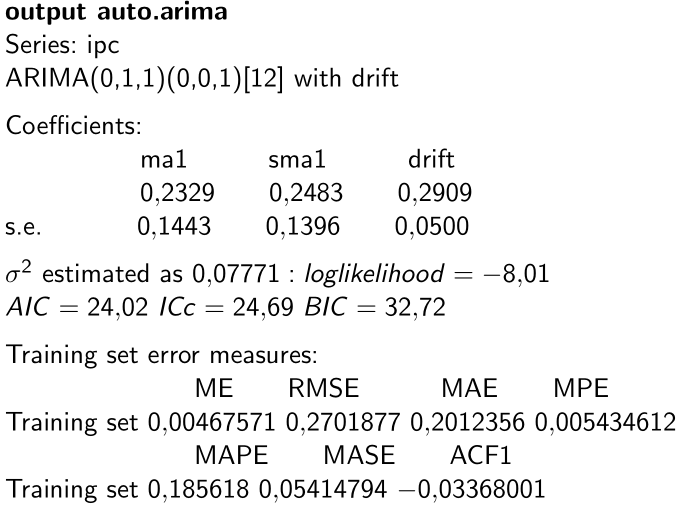
\includegraphics[width=\linewidth]{pronosticoAutoarimaD62.png}}
	\caption{Pronóstico auto ARIMA}\label{fig26}
\end{figure}

%\end{frame}

%---------------------------------------------------------
%---------------------Slide 63--------------------------
%\begin{frame}
%\frametitle{Ejemplo IPC en Chile}
%\textbf{Inverse MA roots  - auto.arima}\\
\vspace{4mm}	
\begin{figure}[H]
	\centering
	\textbf{Inverse MA roots - auto.arima}\par\medskip
	\fcolorbox{green}{blue}{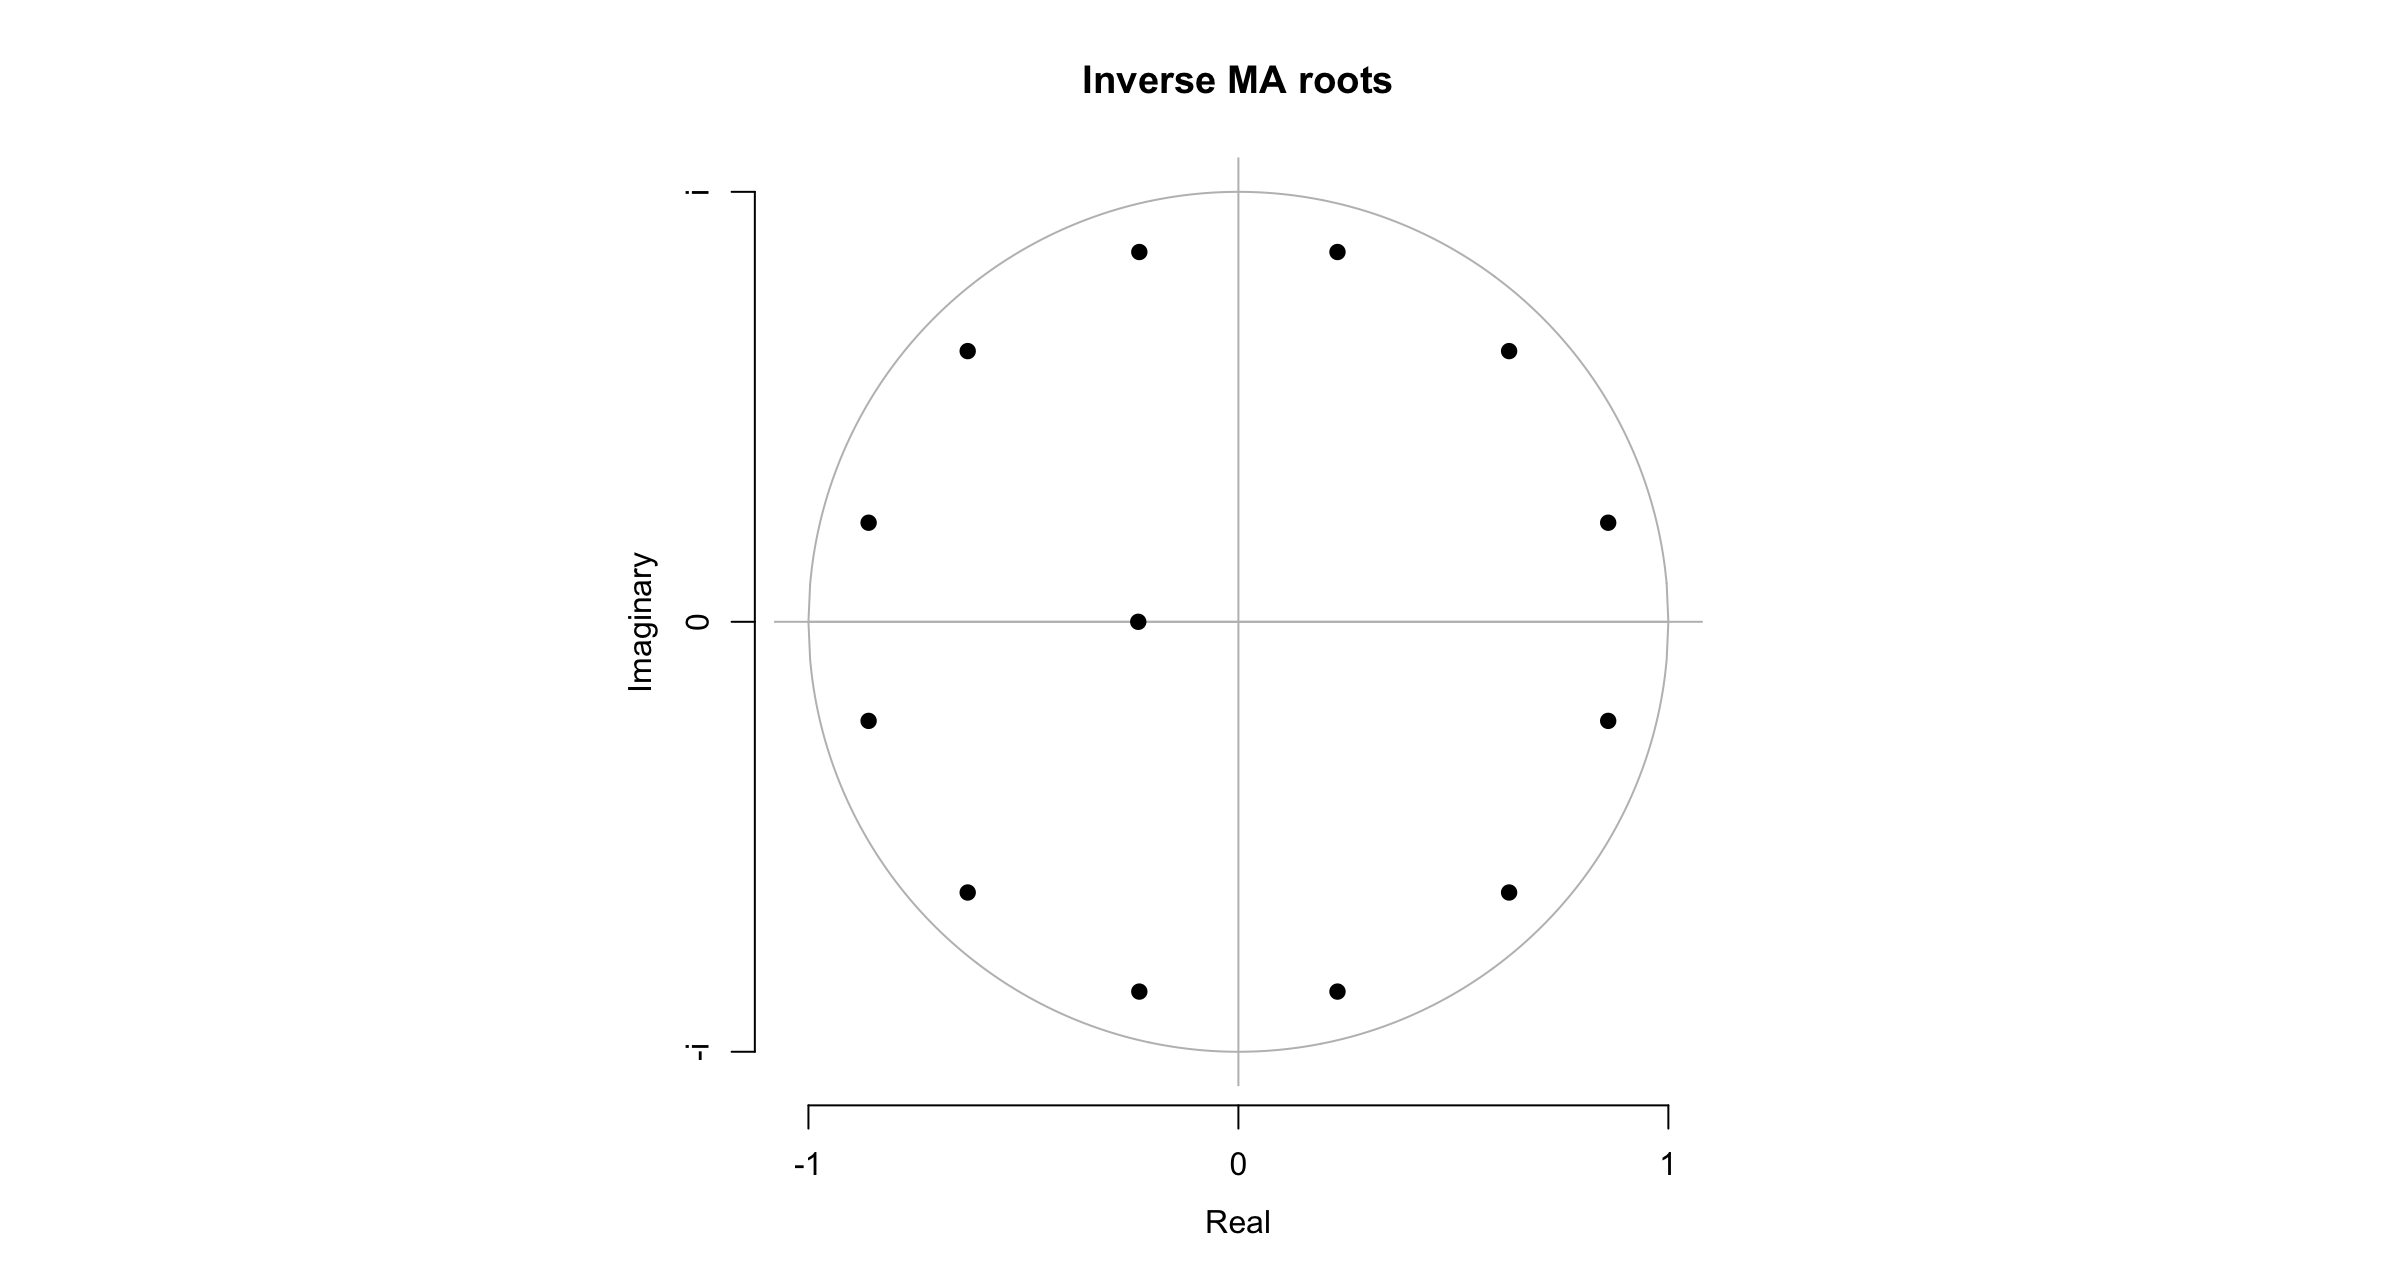
\includegraphics[width=\linewidth]{maroots.png}}
	\caption{Soluciones de ecuación característica - Representación de circulo unitario}\label{fig}
\end{figure}

%\end{frame}

%---------------------------------------------------------
%---------------------Slide 64--------------------------
%\begin{frame}
%\frametitle{Ejemplo IPC en Chile}
%\textbf{Pron\'ostico auto.arima}\\
\vspace{4mm}	
\begin{figure}[H]
	\centering
	\textbf{Forecasts from ARIMA(0,1,1)(0,0,1)[12] with drift}\par\medskip
	\fcolorbox{green}{blue}{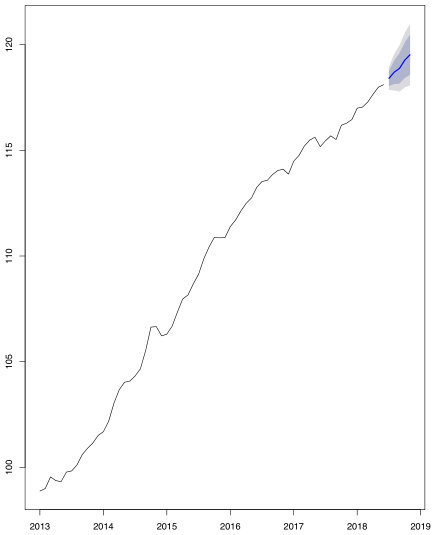
\includegraphics[width=\linewidth]{forecastipc.png}}
	\caption{Ejemplo IPC en Chile: Forecast de modelo auto.arima}\label{fig27}
\end{figure}

%\end{frame}
%\end{section}
%---------------------------------------------------------
%---------------------Slide 65--------------------------
%\begin{section}{Metodolog\'{\i}a de Estimaci\'on de un Modelo ARIMA}
%\begin{frame}
\pagebreak\section{Metodolog\'{\i}a de Estimaci\'on de un Modelo ARIMA}
%\frametitle{Etapas de Estimaci\'on de un Modelo ARIMA}
\subsection{Etapas de Estimaci\'on de un Modelo ARIMA}

%\only<1->{
\begin{itemize}
\item[1] \textbf{Recolecci\'on de datos}: Es recomendable disponer de a lo menos 50 datos, y en el caso de series mensuales, es conveniente trabajar con entre seis y diez a\~nos de datos.
\item[2] \textbf{Representaci\'on gr\'afica de la serie}: Resulta de gran utilidad disponer de diversos gr\'aficos de la serie y sus transfromaciones para decidir sobre la estacionariedad de la misma.
\item[3] \textbf{Transformaci\'on de la serie}: La transformaci\'on de la serie es muchas veces necesaria en caso de encontrarnos con no-estacionaridad.
\item[4] \textbf{Eliminaci\'on de la tendencia}: Al comprobarse gr\'aficamente la existencia de una tendencia, esta debe ser eliminada usando como vimos primeras diferencias, e incluso dos diferencias para una tendencia no lineal.
\item[5] \textbf{Identificaci\'on del modelo}: Se debe determinar el tipo de modelo m\'as adecuado, es decir, el orden de los procesos autorregresivos y de medias m\'oviles de las componentes regular y estacional. Se suelen seleccionar varios modelos alternativos, estimarlos, y contrastarlos, antes de modelar definitivamente la serie.
\item[6] \textbf{Estimaci\'on de los coeficientes del modelo}: A partir del modelo elegido se procede a la estimaci\'on de sus par\'ametros.
\item[7] \textbf{Contraste de validez conjunta del modelo}: Se utilizan los diversos criterios y procedimientos vistos anteriormente para valorar el modelo o modelos seleccionados: test de significancia de par\'ametros, criterios de informaci\'on, covarianzas entre estimadores, coeficiente de correlaci\'on, $R^2$, i.e. suma de cuadrados de errores, etc.
\item[8] \textbf{An\'alisis detallado de los errores}: Los errores extra-muestrales del modelo son determinantes para una valoraci\'on final del modelo. Las diferencias entre valores reales y estimados por el modelo son determinantes para una evaluaci\'on final del modelo.
\item[9] \textbf{Selecci\'on del modelo}: Analizando los resultados de las fases anteriores se decidir\'a sobre el modelo adoptado. Si ninguno de los modelos estudiados nos proporciona resultados suficientemente satisfactorios se vuelve a la etapa 3, revisando todas las decisiones adoptadas.
\item[10] \textbf{Predicci\'on}: Se tomar\'a el modelo v\'alido como f\'ormula inicial de predicci\'on. Ser\'a necesario comparar las predicciones con los valores ya conocidos y, posteriormente, analizar los errores extramuestrales.
\end{itemize}
%}
%
%
%\end{frame}


%---------------------------------------------------------
%---------------------Slide 66--------------------------
%\begin{frame}
%\frametitle{Etapas de Estimaci\'on de un Modelo ARIMA}
%
%\only<1->{
%\begin{itemize}
%\item[5] \textbf{Identificaci\'on del modelo}: Se debe determinar el tipo de modelo m\'as adecuado, es decir, el orden de los procesos autorregresivos y de medias m\'oviles de las componentes regular y estacional. Se suelen seleccionar varios modelos alternativos, estimarlos, y contrastarlos, antes de modelar definitivamente la serie.
%\item[6] \textbf{Estimaci\'on de los coeficientes del modelo}: A partir del modelo elegido se procede a la estimaci\'on de sus par\'ametros.
%\item[7] \textbf{Contraste de validez conjunta del modelo}: Se utilizan los diversos criterios y procedimientos vistos anteriormente para valorar el modelo o modelos seleccionados: test de significancia de par\'ametros, criterios de informaci\'on, covarianzas entre estimadores, coeficiente de correlaci\'on, $R^2$, i.e. suma de cuadrados de errores, etc.
%\end{itemize}
%}

%\end{frame}

%---------------------------------------------------------
%---------------------Slide 67--------------------------
%\begin{frame}
%\frametitle{Etapas de Estimaci\'on de un Modelo ARIMA}
%
%\only<1->{
%\begin{itemize}
%\item[8] \textbf{An\'alisis detallado de los errores}: Los errores extra-muestrales del modelo son determinantes para una valoraci\'on final del modelo. Las diferencias entre valores reales y estimados por el modelo son determinantes para una evaluaci\'on final del modelo.
%\item[9] \textbf{Selecci\'on del modelo}: Analizando los resultados de las fases anteriores se decidir\'a sobre el modelo adoptado. Si ninguno de los modelos estudiados nos proporciona resultados suficientemente satisfactorios se vuelve a la etapa 3, revisando todas las decisiones adoptadas.
%\item[10] \textbf{Predicci\'on}: Se tomar\'a el modelo v\'alido como f\'ormula inicial de predicci\'on. Ser\'a necesario comparar las predicciones con los valores ya conocidos y, posteriormente, analizar los errores extramuestrales.
%\end{itemize}
%}
%
%\end{frame}

%---------------------------------------------------------
%---------------------Slide 68--------------------------
%\begin{frame}
%\frametitle{Resumen de los pasos de Box-Jenkins}
\pagebreak\section{Resumen de los pasos de Box-Jenkins}

\begin{figure}[H]
	\centering
	\textbf{Resumen de los pasos de Box-Jenkins}\par\medskip
	\fcolorbox{green}{blue}{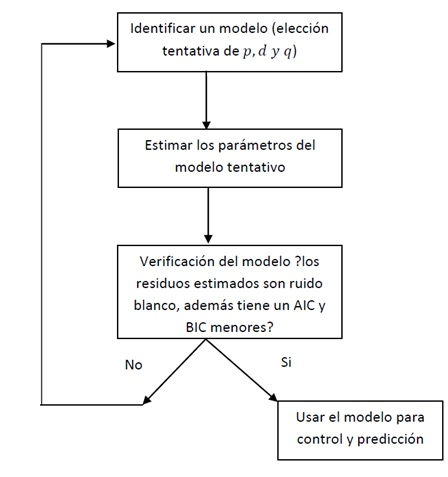
\includegraphics[width=\linewidth]{box_jenkins.png}}
	\caption{Metodología de Box-Jenkins}\label{fig30}
\end{figure}

%\end{frame}
%
%\end{section}

%---------------------------------------------------------
%---------------------Slide 69--------------------------

%\begin{section}{Tarea 2}
%\begin{frame}
%\frametitle{Tarea 2}
\pagebreak\section{Tarea 2}
\begin{mdframed}[style=MyFrame]
Calibrar y evaluar los siguientes modelos para el precio de un commodity (0 activo en \'ultimo caso) a su eleci\'on:\\
\textbf{1.} Camino aleatorio sin drift.,\\
\textbf{2.} Camino aleatorio con drift.\\
\textbf{3.} Promedio de los \'ultimos 5 a\~nos.\\ 
\textbf{4.} Promedio de los \'ultimos 10 a\~nos.\\
\textbf{5.} ARIMA(1,1,0).\\
\textbf{6.} ARIMA(0,1,1).,\\ 
\textbf{7.} ARIMA(1,1,1).,\\ 
\textbf{8.} AR(1).,\\ 
\textbf{9.} AR(2).,\\
\textbf{10.} AR(3).\\
\textbf{11.} $\alpha$ constante, $\psi$ = 1 y $\delta$ sigue un camino aleatorio.\\
\textbf{12.} $\psi$=1,$\delta$=0 y ?sigue un camino aleatorio.\\
\textbf{13.} $\alpha$ constante, $\delta$ y $\psi$ siguen caminos aleatorios con innovaciones independientes.\\
\textbf{14.} $\delta$ = 0, $\alpha$ y $\psi$ siguen caminos aleatorios con innovaciones independientes.\\ 
\textbf{15.} $\alpha$ constante, $\delta$ = 0 y $\psi$ sigue un camino aleatorio.\\
\textbf{16.} $\alpha$, $\delta$ y $\psi$ siguen caminos aleatorios con innovaciones independientes.\\
\textbf{17.} $\alpha$ constante, $\delta$ = 0 y $\psi$ sigue un AR(1).\\
\textbf{18.} $\alpha$ y $\delta$ constantes, $\psi$ sigue un AR(1).\\
\vspace{4mm}	
Basarse en paper anexo.
\end{mdframed}
%\end{frame}
%\end{section}






\curinstructor{Marcelo Villena Chamorro PhD.}

\bibliography{TS_ref_1}

\end{document}